\documentclass[a4paper,12pt,twoside,onecolumn,final,openright,titlepage]{book}%Configuración de la clase... Cambiar draft-->final cuando esté terminado.
\usepackage[utf8]{inputenc}
\usepackage[a4paper,margin=0.2\textwidth]{geometry}%Márgenes
\usepackage[spanish]{babel}

\usepackage{amsmath,amsfonts,amssymb,mathtools}
\usepackage{bm}
\usepackage{tabto}
\usepackage{tabularx}
\usepackage{upgreek}
\usepackage{tipa}
\usepackage{scalerel}
\usepackage{enumitem}
\usepackage[table,xcdraw]{xcolor}
\usepackage{multirow}

\usepackage{graphicx,float}
\usepackage[justification=centering]{caption}
\usepackage[list=true]{subcaption}
\graphicspath{ {Images} }
\usepackage[pdftex,urlcolor=black]{hyperref}
\hypersetup{colorlinks=true,linkcolor=black,citecolor=black}
\addto\captionsspanish{
\renewcommand*\contentsname{Índice de contenidos}
\renewcommand*{\listfigurename}{Índice de Figuras y Tablas}
\renewcommand*{\listtablename}{Índice de símbolos}
\renewcommand*{\spanishtablename}{Tabla}
\renewcommand\bibname{Referencias}
}

\def\table{\def\figurename{Tabla}\figure}
\let\endtable\endfigure 


%%%%%%%%%%%%%%%%%%%%%%%%%%%%%%%%%%%%%%%%%%%%%%%%%%%%%%%%%%%%%%%%%%%%%%%
%% Carátula 
%%%%%%%%%%%%%%%%%%%%%%%%%%%%%%%%%%%%%%%%%%%%%%%%%%%%%%%%%%%%%%%%%%%%%%%
\renewcommand{\maketitle}[0]{%
  \thispagestyle{empty}
    \vspace{-1cm}
    \begin{center}
      \begin{minipage}[t]{0.2\linewidth}
        
\includegraphics[height=1\linewidth]{Images/logos/logo_univ.eps}
      \end{minipage}      
      \hfill
      \begin{minipage}[t]{0.58\linewidth}
        \begin{center}%

          \vspace{-2cm}
          \textsc{\small Universidad Nacional de La Plata}\\
          \textsc{\small Facultad de Ingeniería}\\
          \textsc{\small Departamento de Electrotecnia}
          
        \end{center}
      \end{minipage}      
      \hfill
      \begin{minipage}[t]{0.2\linewidth}
        
\includegraphics[width=1.1\linewidth]{Images/logos/logo_fiunlp.png}
      \end{minipage}\\
    \end{center}
    \vspace{1cm}
    \begin{center}
      {\LARGE \textbf{Estudio e Implementación del Protocolo RTCM para DGNSS en Tiempo Real}}
    \end{center}
    \vspace{1cm}
    \begin{center}
      \begin{minipage}[t]{0.9\linewidth}
        \begin{center}
          \textsc{Tesina de grado presentada a la Facultad de Ingeniería de
            la Universidad Nacional de La Plata
            por}\\\vspace{0.5cm}{\Large
            Juan Fermín Llorente}\\\vspace{0.5cm}\textsc{en cumplimiento parcial
            de los requerimientos\\ para la obtención del título
            de\\Ingeniero en Telecomunicaciones.}
%            para obtener el título de Ingeniero en Telecomunicaciones.
        \end{center}
      \end{minipage}
    \end{center}

    \vspace{2cm}

    \begin{center}
      \textsc{Directores}
      \begin{minipage}[t]{0.9\linewidth}
        
        Ing. Ernesto M. López %
        \dotfill{} %
        UIDET SENyT, FI-UNLP %
        
        Ing. Javier A. Smidt %
        \dotfill{} %
        UIDET SENyT, FI-UNLP %

      \end{minipage}

      \vspace{1cm}

      \textsc{Tribunal}\\
      \begin{minipage}[t]{0.9\linewidth}
		Ing. Javier A. Smidt %
        \dotfill{} %
        \textit{Director de Carrera} %
        
        Dr. Ing. P. Agustín Roncagliolo %
        \dotfill{} %
        Cátedra \textit{Tesina de Grado} %
        
        Ing. Ernesto M. López %
        \dotfill{} %
        \textit{Dirección del Trabajo} %
      \end{minipage}

    \begin{minipage}[t]{0.9\linewidth}
        \vspace{.5cm}
        \centering
        
\includegraphics[width=0.6\textwidth]{Images/logos/logoSenytByN.png}\\
%        UIDET Sistemas Electrónicos de Navegación y Telecomunicaciones (SENyT)
    \end{minipage}
    
%    \vspace{2cm}
    \vfill 

    \begin{minipage}[t]{0.9\linewidth}
    \centering
        La Plata\\
        5 de Diciembre, 2022
    \end{minipage}
    \end{center}
}

\begin{document}
\pagestyle{empty}
\maketitle

\frontmatter
\renewcommand{\chaptermark}[1]{\markboth{\MakeUppercase{#1}}{}}	% Se le saca el num de cap al header.
\cleardoublepage
\pagestyle{headings}
\chapter*{Resumen/Abstract}
\addcontentsline{toc}{chapter}{Resumen/Abstract}
%\pagenumbering{arabic}
	En este trabajo se estudian los aspectos más importantes del estándar RTCM para el envío de mensajes entre receptores GNSS realizando posicionamiento diferencial en tiempo real. Se decide trabajar con un mensaje de la estación de referencia y un mensaje con observables crudos de pseudorango y fase de portadora. Estos mensajes son tipificados por el estándar e identificados como Tipo 1005 y Tipo 1074, siendo este último un mensaje particular para el sistema GPS. 

	Se realizan ensayos DGPS con línea de base nula utilizando receptores comerciales y obteniendo soluciones con la precisión esperada. Se implementa en un sistema embebido la transmisión de los mensajes ya mencionados mediante una interfaz cableada. Además, se replican los ensayos con línea de base nula utilizando como estación de referencia el receptor de diseño y desarrollo propio del lugar de trabajo donde se implementó la transmisión de los mensajes. Se mantiene al receptor comercial como el receptor que realiza el procesamiento diferencial y se observa la ganancia que presenta un enfoque diferencial en términos de la precisión obtenida en las soluciones de posición. Se valida el desarrollo mediante un ensayo diferencial en tiempo real con los receptores separados y comunicándose de manera inalámbrica.\\
\textbf{\textit{Index Terms:}} \textit{GNSS}, \textit{posicionamiento relativo}, \textit{estándar RTCM}.

\vspace{0.7cm}
\noindent\rule{3.5cm}{0.4pt}
\vspace{0.7cm}

	The present work consists of the study of the most important aspects that the RTCM standard describes for the communication between GNSS receivers performing differential positioning in real time. It is decided to work with a message for the reference station and one with raw pseudorange and phaserange observables. These messages are typified by the standard and identified as Type 1005 and Type 1074, being the last one mentioned a particular message for the GPS system.
	
	DGPS tests are done with zero baseline setup and using commercial receivers, solutions with expected accuracy are obtained. The wired transmission of the messages mentioned above is implemented in an embedded system. Further, tests with zero baseline are replicated, using the receiver designed and integrated previously in the workplace as reference station. This is the receiver where the RTCM messages transmission was implemented. The commercial receiver performing differential processing is mantained and the gain, in terms of accuracy in the position solution, that a differential approach obtains is evident. The validation of the work is done by a real time differential setup with a wireless communication between the two receivers that are physically separated.\\
\textbf{\textit{Index Terms:}} \textit{GNSS}, \textit{relative positioning}, \textit{RTCM standard}.
\chapter*{Agradecimientos}
\addcontentsline{toc}{chapter}{Agradecimientos}
Primero quiero dar las gracias a mis directores, Javier Smidt y Ernesto López, por la confianza que me depositaron y el constante acompañamiento, tanto técnico como humano. A todo el SENyT en general por haber hecho de este trabajo un proceso disfrutable y de constante aprendizaje. No puedo dejar de mencionar a Germán Scillone, Agus Catellani y Santi Rodríguez, que sin ellos mis aportes al código del receptor hoy no compilarían.

A todos los profesores apasionados que me contagiaron el amor por las telecomunicaciones. En especial a Adrián Carlotto, que fue el primero de ellos y una gran fuente de confianza para tomar la decisión de seguir, la que para mí, es la especialidad más apasionante de la ingeniería. También a Javier y Agustín Roncagliolo que me abrieron las puertas para seguir formando mi camino en el mundo GNSS.\\

Gracias a todos los amigos y amigas que me dió la facultad, electrónicos, aeronáuticos e hidráulicos, hicieron que esta etapa sea inolvidable. No puedo evitar pensar en mis amigos de la infancia y algunos más nuevos, Tobi, Martín, Facu, Cami, Chiari, Kevin, Juani, Luci y Nacho, por estar en todo momento. A la familia Pérez-Arrua; Milton y Santi por todas las charlas. A mi familia en Roca por recibirme siempre que necesité volver. Por último, el agradecimiento más grande a Felipe y a mis padres, por apoyarme incondicionalmente y permitirme hacer lo que me apasiona.\\

Quiero cerrar estas palabras remarcando mis convicciones, no solo agradeciendo a la UNLP, si no también a todo lo que ello representa, un país que apuesta a la ciencia y a la educación. Gracias a la educación pública, libre y gratuita por haberme brindado una formación de privilegio.

\cleardoublepage
\phantomsection
\addcontentsline{toc}{chapter}{Índice de contenidos}
\tableofcontents


\cleardoublepage
\phantomsection
\renewcommand{\chaptermark}[1]{\markboth{\MakeUppercase{#1}}{}}	% Se le saca el num de cap al header.
\chapter*{Índice de símbolos}\chaptermark{Índice de símbolos}
\addcontentsline{toc}{chapter}{Índice de símbolos}
\noindent\textbf{ARP:} \textit{Antenna Reference Point}, Punto de Referencia de la Antena.\\
\textbf{BART:} \textit{Bayesian Amiguity Resolution Technique}.\\
\textbf{BPSK:} \textit{Binary Phase Shift Keying}, Modulación Binaria por Desplazamiento de Fase.\\
\textbf{BRSD:} \textit{Between Receivers Simple Differences}, Simples Diferencias Entre Receptores.\\
\textbf{BSSD:} \textit{Between Satellite Simple Differences}, Simples Diferencias Entre Satélites.\\
\textbf{CDMA:} \textit{Code Division Multiple Access}, Acceso Múltiple por División de Código.\\
\textbf{CPU:} \textit{Central Processing Unit}, Unidad Central de Procesamiento.\\
\textbf{CRC:} \textit{Cyclic Redundancy Check}, Control de Redundancia Cíclica.\\
\textbf{DD:} \textit{Double Differences}, Dobles Diferencias.\\
\textbf{DGNSS:} \textit{Differential GNSS}, GNSS diferenciales.\\
\textbf{DGPS:} \textit{Differential GPS}, GPS diferencial.\\
\textbf{DLL:} \textit{Delay Lock Loop}, Lazo de Enganche de Retardo.\\
\textbf{DOP:} \textit{Dilution Of Precision}, Dilución de Precisión.\\
\textbf{DSP:} \textit{Digital Signal Processing}, Procesamiento Digital de Señales.\\
\textbf{DSSS:} \textit{Direct Sequence Spread Spectrum}, Espectro Expandido de Secuencia Directa.\\
\textbf{ECEF:} \textit{Earth Centered Earth Fixed}, Centrado en la Tierra con la Tierra Fija.\\
\textbf{ENU:} \textit{East-North-Up}, Este-Norte-Arriba.\\
\textbf{FDMA:} \textit{Frequency Division Multiple Access}, Acceso Múltiple por División de Frecuencia.\\
\textbf{FPGA:} \textit{Field Programmable Gate Array}, Matriz de Puertas Lógicas Programable en Campo.\\
\textbf{GNSS:} \textit{Global Navigation Satellite Systems}, Sistemas Globales de Navegación por Satélite.\\
\textbf{GPS:} \textit{Global Positioning System}, Sistema Global de Posicionamiento.\\
\textbf{LAMBDA:} \textit{Least-squares AMBiguity Decorrelation Approach}.\\
\textbf{MEO:} \textit{Medium Earth Orbit}, Orbita Terrestre Media.\\
\textbf{MSM:} \textit{Multiple Signal Messages}, Mensajes de Múltiples Señales.\\
\textbf{PLL:} \textit{Phase Lock Loop}, Lazo de Enganche de Fase.\\
\textbf{PPS:} \textit{Pulse Per Second}, Pulso Por Segundo.\\
\textbf{PRN:} \textit{Pseudorandom Noise}, Ruido Pseudo Aleatorio.\\
\textbf{RF:} \textit{Radio Frequency}, Radiofrecuencia.\\
\textbf{RINEX:} \textit{Receiver INdependent EXchange}, Intercambio Independiente del Receptor.\\
\textbf{RTCM:} \textit{Radio Technical Commission for Maritime Services}, Comisión Técnica de Radio para Servicios Marítimos.\\
\textbf{RTK:} \textit{Real Time Kinematics}, Cinemática de Tiempo Real.\\
\textbf{RTOS:} \textit{Real Time Operative System}, Sistema Operativo de Tiempo Real.\\
\textbf{SD:} \textit{Simple Differences}, Simple Diferencias.\\
\textbf{SVID:} \textit{Space Vehicle Identifier}, Identificador de Vehículo Espacial.\\
\textbf{TOA:} \textit{Time Of Arrival}, Tiempo de Arribo.\\
\textbf{UART:} \textit{Universal Asincronus Receiver Transmitter}, Transmisor-Receptor Asíncrono Universal.\\
\textbf{USB:} \textit{Universal Serial Bus}, Bus Serie Universal.\\

\cleardoublepage
\phantomsection
\addcontentsline{toc}{chapter}{Índice de Figuras y Tablas}
\listoffigures


\cleardoublepage
\phantomsection
\addcontentsline{toc}{chapter}{Introducción}
\chaptermark{Introducción}
\chapter*{Introducción}
%Los Sistemas Satelitales de Navegación Global (GNSS) presentan en la actualidad un uso extendido y creciente, demostrando ser de gran importancia en aplicaciones de navegación aérea, satelital, terrestre y marítima, para agrimensura y mapeo, servicios basados en localización, entre otros usos civiles, científicos y militares. En particular, en el campo de aplicaciones aeroespaciales, la utilización de receptores GNSS resulta idónea debido al costo y nivel de precisión en tiempo real que los mismos proporcionan. Misiones de observación terrestre realizadas por satélites en órbita baja, utilizando diversos tipos de instrumentos, permiten generar datos útiles para campos como la agricultura, meteorología, monitoreo de desastres naturales, entre otros. En dicho tipo de misiones, los receptores GNSS proporcionan una solución de navegación a bordo en tiempo real, la cual permite tanto el control de la órbita como la localización necesaria para la generación de datos de ciencia.
%
%Con el paso del tiempo, existe una creciente tendencia a la segmentación de las misiones espaciales, con el objetivo de distribuir los instrumentos en múltiples satélites de menor tamaño y costo, incrementando a su vez la robustez y la adaptabilidad de las misiones. En estos casos, resulta de vital importancia la implementación de sistemas de navegación relativa, necesario para el control del vuelo en formación de los satélites. Ejemplos recientes de este tipo de arquitecturas segmentadas y de satélites en vuelo en formación son las misiones TerraSAR-X/TanDEM-X de radar de apertura sintética, GRACE y GRACE-FO de gravimetría, PRISMA, y los nanosatélites CanX-4 y 5 de demostración tecnológica, entre otros. El nivel de precisión requerido por estos sistemas de navegación es, en general, superior al obtenido mediante la navegación absoluta de cada uno de los satélites de la formación. Esto hace necesario el uso de técnicas diferenciales empleando las mediciones crudas de fase de portadora, las cuales poseen un nivel de ruido del órden de los milímetros, pero con el inconveniente de ser ambiguas en un número entero de ciclos de portadora.
%
%	Resulta de interés aplicar estas técnicas diferenciales a bordo en tiempo real, a fin de incrementar la autonomía y la versatilidad en cuanto a las posibles aplicaciones de ciencia. Para esto, la transmisión de las mediciones entre satélites en tiempo real es necesaria. Adicionalmente, otros campos donde la navegación relativa de alta precisión en tiempo real presenta grandes utilidades incluyen la agricultura de precisión, topografía y la navegación autónoma de vehículos, donde un receptor utilizado como estación base transmite correcciones a múltiples receptores móviles o rovers. Estas correcciones son transmitidas en forma de mensajes basados en el estándar RTCM, cuya estandarización permite el empleo de receptores de diferentes características y fabricantes para estas técnicas diferenciales.
\section*{Motivación}
\addcontentsline{toc}{section}{Motivación}
	El presente trabajo se enmarca dentro de los distintos desarrollos llevados a cabo por la UIDET SENyT en torno al desarrollo de receptores GNSS de aplicación espacial. Además del desarrollo, se realiza investigación en distintas áreas dentro de los sistemas GNSS. En particular, existe una fuerte línea de investigación relacionada al posicionamiento diferencial de alta precisión. Resulta de interés poder contar con receptores de desarrollo propio que puedan operar de manera diferencial en tiempo real ya que esto da lugar a probar algoritmos de procesamiento diferencial de desarrollo propio. Al trabajar únicamente con receptores comerciales todo el procesamiento se debe realizar de manera no sincrónica, es decir, con post procesamiento, debido a la imposibilidad de modificar el software de los receptores.
\section*{Objetivos}
\addcontentsline{toc}{section}{Objetivos}
	El objetivo general de este trabajo es el estudio e implementación de técnicas de posicionamiento diferencial utilizando receptores GNSS diseñados y fabricados en el lugar de trabajo. Dichos receptores cuentan actualmente con la capacidad de generar las mediciones crudas necesarias para la aplicación de estas técnicas. Para ello, deberán cumplirse los siguientes objetivos particulares:
\begin{itemize}
	\item Estudiar el estándar RTCM para posicionamiento GNSS relativo.
	\item Replicar ensayos DGNSS con receptores comerciales.
	\item Implementar el enlace de comunicación de los mensajes del protocolo RTCM en un receptor propietario del SENyT y validar el desarrollo mediante un ensayo DGPS en tiempo real.
\end{itemize}	

	El trabajo se estructura de la siguiente manera: \\El Capítulo~\ref{ch:GNSS} presenta los conceptos principales de los Sistemas Globales de Navegación por Satélite. En el Capítulo~\ref{ch:DGNSS} se aplican esos mismos conceptos a un enfoque diferencial para dar lugar a las bases que fundamentan el objetivo principal de este trabajo. Posteriormente se presentan ensayos de posicionamiento relativo entre dos receptores GNSS comerciales, los resultados se pueden encontrar en el Capítulo~\ref{ch:ublox}. El Capítulo~\ref{ch:Qseries} detalla la implementación llevada a cabo en uno de los receptores GNSS propietarios del lugar de trabajo y la validación de esta implementación con la presentación de los resultados se encuentra en el Capítulo~\ref{ch:validacion}. Por último, se termina el trabajo dando las conclusiones generales del mismo junto con propuestas de líneas de trabajo a futuro que surgen a partir de lo aquí desarrollado.
	
\mainmatter
\renewcommand{\chaptermark}[1]{\markboth{\MakeUppercase{\chaptername\ \thechapter.\ #1}}{}}	%Asi es el comando original. "Chapter num. Nombre de capitulo"
\chapter{Sistemas globales de navegación por satélite}\label{ch:GNSS}\chaptermark{GNSS}
	Este capítulo introduce los primeros conceptos para el posicionamiento basado en sistemas de navegación por satélite. Incluye una breve descripción del Sistema de Posicionamiento Global (GPS por sus siglas en inglés) junto con sus señales y las mediciones que pueden obtenerse mediante las mismas. Se hace hincapié en las características de estas señales, analizando las fuentes de error que hay presentes en las mediciones que pueden obtenerse. Si bien el foco de este trabajo está puesto en el sistema GPS, ya que los resultados obtenidos son para el mismo, se desarrollan los conceptos de este capítulo de forma general para cualquiera de los sistemas globales de navegación por satélite..
	
\section{Introducción}
	Los sistemas GNSS (Sistemas Globales de Navegación por Satélite o \textit{Global Navigation Satellite System} en inglés) se basan en el concepto de mediciones de distancia mediante el retardo de propagación de las señales transmitidas por satélites de posicionamiento que orbitan la tierra. Ante la necesidad de poder contar con mecanismos para obtener posición y velocidad de usuarios en la tierra, a la cual se agrega la necesidad de sincronización entre distintos sistemas de referencia temporal, surge la idea e implementación de los sistemas GNSS. Los mismos no han dejado de ser utilizados desde su puesta en funcionamiento debido a que permiten cobertura global para distintas aplicaciones de posicionamiento. Se mencionó que pueden ser utilizados para sincronización de relojes debido a que las señales que transmiten los satélites también tienen información temporal de alta precisión. Además del uso civil, están las aplicaciones científicas o militares, pero existen áreas donde estos sistemas presentan un uso extendido y creciente, tales como la geodesia, seguimiento de fauna, navegación aérea, satelital, terrestre y marítima.
	
\begin{figure}%Se puede agregar un indicador de chip en la imagen.
    \centering
    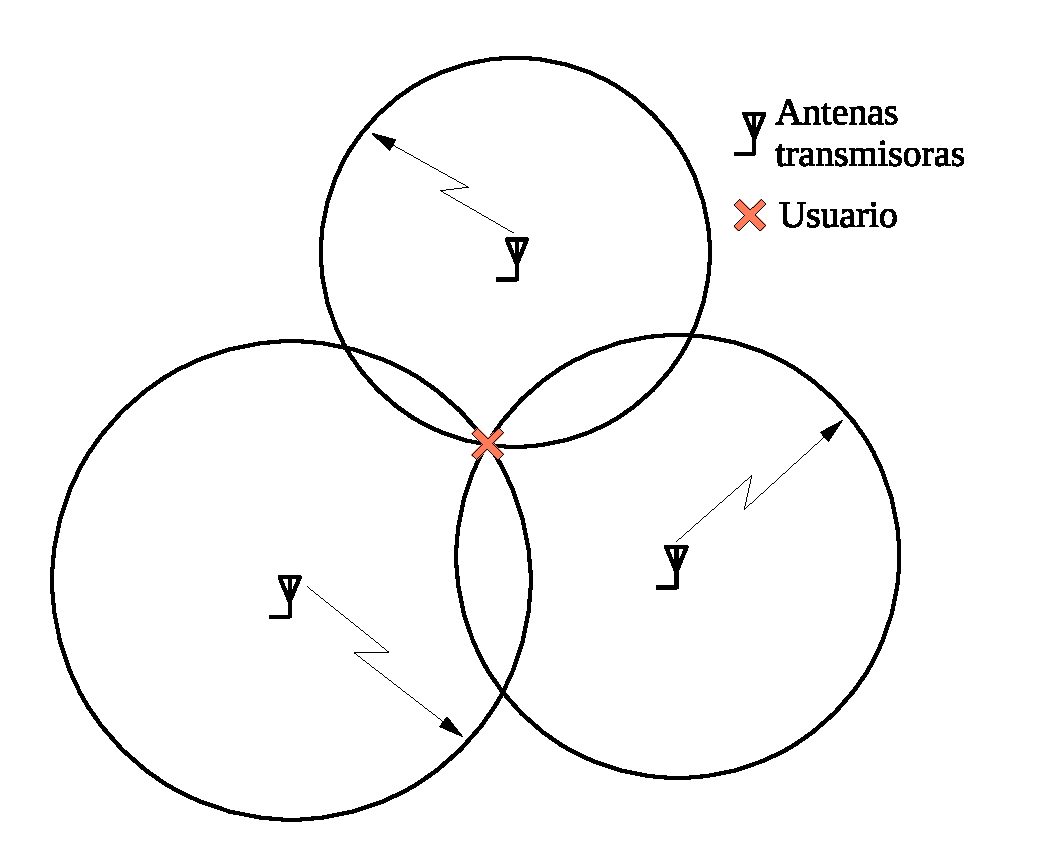
\includegraphics[width=0.8\textwidth]{/GNSS/triangulacion.eps}
    \caption{Resolución de la posición del usuario en dos dimensiones mediante la medición de distancias a los transmisores.}
    \label{fig:triangulacion}
\end{figure}	
	
	El concepto subyacente para poder obtener posición es el de triangulación. El tiempo de arribo (TOA por sus siglas en inglés) determina el instante en el que se recibió la señal; conociendo el instante en el que fue transmitida se puede determinar el tiempo de viaje de la misma. Haciendo uso de la velocidad de propagación de la señal es posible obtener la distancia a la que se encuentra el equipo transmisor. Introduciendo múltiples mediciones con satélites transmitiendo en distintas ubicaciones se puede acotar la ubicación del receptor. En la Fig.~\ref{fig:triangulacion} se puede observar el mecanismo para acotar la solución con un ejemplo en el plano, es decir, en dos dimensiones. En el caso tridimensional, es equivalente, la diferencia resulta en que la solución puntual queda determinada por el punto de intersección de las esferas formadas por la distancia que se midió a cada uno de los satélites involucrados, siempre y cuando se tomen suficientes mediciones para poder resolver la posición de manera unívoca.
	
	Habiendo introducido el concepto de medición de rango mediante TOA, es necesario analizar la sincronización entre las distintas partes que conforman el sistema. Si se busca resolver la posición mediante este concepto, las señales recibidas de los distintos satélites deben estar alineadas. Para esto es necesario poder identificar los instantes de transmisión y que los mismos estén referenciados a un mismo patrón. El instante de tiempo de toma de las observaciones tiene el nombre de época en este contexto. Es evidente que para conseguir esto los relojes de referencia de los satélites y del usuario (llamado receptor anteriormente) deben tener muy alta precisión y sincronización entre ellos. La precisión no es un inconveniente para los satélites GNSS ya que los mismos utilizan relojes atómicos que logran una estabilidad destacable. En cambio, la sincronización del usuario al tiempo del sistema GNSS (al cual deberían estar sincronizados todos los satélites de la constelación), es un tanto más compleja y por ello se analizarán los errores que introducen las fallas en la sincronización.
	
	Existen distintos sistemas GNSS, tales como GPS, \textit{Galileo}, GLONASS o \textit{BeiDou}, cada uno con su respectiva constelación de satélites MEO (\textit{Medium Earth Orbit} u Órbita Circular Intermedia). Todos los satélites de las distintas constelaciones comparten el canal de transmisión, lo cual es posible debido al uso de técnicas de acceso múltiple. En particular, el sistema GPS cuenta con 32 satélites operativos actualmente y como la frecuencia de operación es compartida por todos los satélites, el mismo utiliza acceso múltiple por división de código (CDMA por sus siglas en inglés). En cambio, el sistema GLONASS cuenta con 24 satélites operativos y cada uno transmite dentro de la misma banda de frecuencias multiplexando los canales por frecuencia dentro de esta banda. Esta técnica es conocida como acceso múltiple por división de frecuencia (FDMA por sus siglas en inglés).
	
\section{Características de la señal}\label{sec:senial}
	Las señales transmitidas se encuentran dentro del espectro de las radiofrecuencias. Existen distintos tipos de señales, según se fueron modernizando los sistemas, y en particular los satélites, se han ido sumando nuevas señales. Las características principales que componen a una señal de GPS son la frecuencia de portadora dentro de la banda \textit{L}, el código que hace posible el acceso múltiple y por último el mensaje de navegación.
	
	En cuanto a la frecuencia de portadora de la señal, para aplicaciones civiles se puede diferenciar la frecuencia primaria L1 y frecuencia secundaria L2. Ambas son múltiplos de una frecuencia fundamental $f_0=10.23$\,MHz. La señal en L1 tiene una frecuencia de portadora igual a $154\cdot f_0 = 1.5754$\,GHz y la señal en L2 igual a $120\cdot f_0 = 1.2276$\,GHz. Estas dos señales son las consideradas \textit{legacy} ya que fueron heredadas de los primeros bloques de satélites GPS que se hicieron operativos. También existe una señal en L5, más moderna, pero que no es utilizada a lo largo de este trabajo por lo que solo se la menciona.
	
	Las señales son expandidas en el espectro mediante una secuencia de ruido pseudoaleatoria (PRN por sus siglas en inglés), esta secuencia es el código que ya fue mencionado. Además de presentar la ventaja de permitir el acceso múltiple entre usuarios, las técnicas de espectro expandido de secuencia directa (DSSS por sus siglas en inglés) utilizadas, distribuyen la energía de la señal de cada satélite en todo el ancho de banda disponible. De esta manera es posible mitigar efectos adversos naturales del canal como lo son el ruido o interferencias. Esta última característica generaba gran interés al momento de la creación del sistema GPS, sobre todo cuando se lo pensaba para fines militares. La idea que sustenta esta robustez es que se reparte la potencia de señal en un ancho de banda mucho mayor que el natural de la señal de datos, de tal manera que queda oculta por el piso de ruido presente en el canal. El receptor, que conoce el código con el cual se hizo la expansión, logra recuperar la señal pudiendo incluso considerar a las señales del resto de los satélites como interferencias.
	
	Los mensajes de navegación en GPS se transmiten con una tasa $R_b$ de 50\,bps, como la modulación es BPSK esto resulta en un ancho de banda de 50\,Hz. Los símbolos transmitidos son de 20\,ms de duración con forma de pulso ideal tipo cajón. La información transportada por el mensaje de navegación es la que hace posible computar la posición de cada satélite y tiempo de transmisión de las señales. En los mismos se transmite, entre otras cosas, el mensaje de telemetría, al cual solo tienen acceso usuarios autorizados, términos de corrección de reloj para desafectar errores en la medición y como componente principal, se transmiten las efemérides. Estos últimos dos son indispensables para que el usuario pueda calcular su posición. Las efemérides contienen la información del tiempo del satélite (referenciado al tiempo GPS) y parámetros keplerianos de las órbitas osculantes de los satélites.
	
	Los parámetros keplerianos que se transmiten son un conjunto de datos que permiten caracterizar por completo la órbita de los satélites. Los mismos surgen de una de las formulaciones posibles para el problema de los dos cuerpos que define la trayectoria de un cuerpo orbitando a la tierra. Cabe destacar que estos parámetros tienen variaciones temporales lentas debido a las fuerzas que interactuan entre el satélite y la tierra~\cite{kaplan}, por lo cual tiene sentido que se transmitan a baja tasa en el mensaje de navegación.
	
	En términos generales, la polaridad de cada símbolo rectangular estará dada por el bit de información de navegación a transmitir. Luego se expande esta señal mediante el producto de la amplitud de cada símbolo con el código, la modulación por desplazamiento de fase de la señal resultante estará dominada por las transiciones del código (Fig.~\ref{fig:PRN}). Cabe destacar que cada transición del código es denominada \textit{chip}. Es evidente que la tasa resultante de la señal BPSK multiplicada por el código es mucho mayor que la de la señal original, ya que en cada transición de símbolo tiene múltiples transiciones de \textit{chip}. La señal de espectro expandido tiene una tasa igual a la tasa de \textit{chip} $R_c$ tal que $R_c \gg R_b$, resultando en una expansión en el espectro.
\begin{figure}%Se puede agregar un indicador de chip en la imagen.
    \centering
    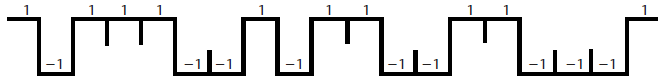
\includegraphics[width=0.8\textwidth]{/GNSS/codigoPRN.eps}
    \caption{Ejemplo de las distintas partes que conforman a la señal GPS.}
    \label{fig:PRN}
\end{figure}

	Este mecanismo implica que el receptor conozca con exactitud el código utilizado en la expansión para poder multiplicar a la señal por el mismo, considerando sincronización perfecta, y así recuperar la señal original. Este proceso se puede interpretar como la compresión de la señal expandida al momento de la transmisión, y en la recepción es donde se recupera solo la señal de interés.
	
	Como ya fue mencionado, el sistema utiliza CDMA para multiplexar las señales de los distintos satélites. Cada satélite tiene una secuencia PRN que debe cumplir con las características de presentar autocorrelación muy similar a la de un proceso de ruido blanco, para su correcta recuperación en el receptor cuando hay sincronización. Y además debe tener muy baja intercorrelación con los códigos del resto de los satélites. Esta última condición es necesario extenderla para que cada PRN tenga baja intercorrelación con todos los posibles desplazamientos de los restantes códigos del sistema. Esto se debe a las variaciones de TOA de las diferentes señales y por el mecanismo de medición de tiempo de viaje de la señal que se detallará posteriormente. Un tipo de secuencias PRN que presentan estas características son las secuencias \textit{Gold}~\cite{proakis}. El sistema GPS utiliza en una de sus señales estas secuencias, pero en el resto de las señales se utilizan secuencias de máximo largo o variantes más complejas. Si los distintos códigos fueron diseñados (o elegidos) correctamente, las interferencias del resto de las señales no deseadas pueden ser consideradas como ruido aditivo a la señal de interés.
	
	Ya se introdujo el mecanismo de multiplexado de las señales de cada satélite y se detallaron algunos aspectos de las señales GPS. Las señales civiles mencionadas pueden estar expandidas por distintos códigos, que en conjunto con la frecuencia de portadora son los dos parámetros que le dan nombre a los observables obtenidos. Estos nombres están estandarizados según el estándar RINEX (Formato de Intercambio Independiente del Receptor o \textit{The Receiver Independent Exchange Format})~\cite{rinex}. Dentro de estos códigos se pueden mencionar el código $C/A$ (por \textit{Coarse Adquisition}) y el código $P$.
\begin{itemize}
	\item Código C/A: Es referido como el código grueso, y es de la familia de códigos de largo 1023. Tiene una tasa de 1.023 Mchips/s por lo tanto tiene un periodo de \textit{chip} igual a $1\mu$\,s.
	\item Código P: Este código se repite una sola vez por semana, al comienzo de la semana GPS (dentro del sistema de tiempo GPS), por eso se lo menciona como código largo o de precisión. Tiene un largo de $6,187104\cdot 10^{12}$ chips y se transmite a una tasa diez veces mayor que la del código C/A.
\end{itemize}

	La señal a la frecuencia L1 con código C/A es denominada L1C. En un plan de modernización del sistema GPS se agrega una nueva señal civil denominada L2C, que es una versión mejorada de L1C pero en la frecuencia L2. La misma agrega posibilidad de corrección de efectos atmosféricos al combinarla con L1C, estos aspectos se tratarán posteriormente en este capítulo. Los códigos que realizan la expansión de esta señal son el código $M$ y el código $L$, ambas secuencias de máximo largo. Donde el código $M$ es un código de uso militar más moderno que el código $P$ y el código $L$ tiene la particularidad de no contar con información del bit de datos.
%	Según el estándar RINEX [cita RINEX] (\textit{The Receiver Independent Exchange Format}) se especifican códigos de observación para las señales. En particular la señal en L1 con código $C/A$ es denominada $X1C$ y la misma señal pero en L2 es denominada $X2C$, donde la $X$ indica qué tipo de observación se hizo. Pudiendo ser estas pseudorango (C), fase de portadora (L), doppler (D) y potencia de señal (S).
\section{Formación de los observables}\label{sec:observables}
	  Para poder obtener una solución de posición es necesario calcular los observables a partir de las mediciones que puede realizar el receptor. En otras palabras, el receptor no tiene manera de medir distancia recorrida por una señal, pero sí puede medir el retardo que se produjo en la señal entre la transmisión y la recepción para formar un observable de pseudorango. Las mediciones naturales del receptor son la fase del código réplica generado en el receptor, fase de la portadora réplica (con el receptor enganchado en fase a la portadora transmitida por el satélite) y frecuencia de la portadora réplica (con el receptor ahora enganchado en frecuencia). A partir de estas es posible obtener las mediciones de los observables de pseudorango, fase de portadora y desviación de frecuencia de portadora o \textit{doppler}. Este último no es utilizado a lo largo de este trabajo por lo que no se hará hincapié en el mismo.
	
\subsection{Medición de pseudorango}
	La formación del pseudorango se basa en la medición del tiempo de viaje de la señal y es aquí donde se aprovechan las características de los códigos mencionados en la Sección~\ref{sec:senial}. El receptor debe conocer el código (ya sea C/A o L2C) asociado al satélite y señal que quiere recibir. Este se utiliza para generar una réplica del mismo en el lazo de enganche de retardo (DLL por sus siglas en inglés) del receptor de manera de poder comparar el desfasaje que existe entre el código de la señal recibida con el generado internamente, obteniendo el tiempo de viaje de la señal. Por esto es que la medición natural que fue mencionada es la de la fase del código réplica. Ambos códigos se generan internamente en satélite transmisor al inicio de la semana GPS y al medir el desfasaje entre la réplica y el recibido se posiciona el TOA dentro de la semana GPS. En el caso del código C/A hay una ambigüedad de 1 ms debido a su periodo, pero se obtiene el TOA bajo estas condiciones y haciendo uso del mensaje de navegación se logra una medida absoluta. En el caso del código P se obtiene una ubicación absoluta dentro de la semana GPS, no existe tal ambigüedad. Para medir el desfasaje, el receptor desplaza en tiempo la réplica hasta lograr correlación entre ambas señales, por esto es importante que la intercorrelación entre los códigos sea baja para todos los desplazamientos de los mismos. De esta manera se evitan falsas detecciones, solo consiguiendo un pico de correlación cuando hay sincronización con el código del satélite que se espera recibir.
	
	Sumado al rango geométrico que se obtiene del tiempo de viaje, existen términos de error adicionales debido a efectos atmosféricos, por sincronización entre relojes del receptor y satélites, y distintos retardos que se pueden presentar en la medición. La ecuación de observación con medición de pseudorango es 
\begin{align}\label{ec:obs_pseudorango}
	p_{r,j}^s(t) = \rho_r^s(t) + \xi_{r,j}^s + c\left(d_{r,j}-d_j^s\right) + c\left(dt_r(t)-dt^s(t)+\delta t^{rel}(t)\right)& \\ 
	+ I_{r,j}^s(t) + T_r^s(t) +e_{r,j}^s(t)& \ . \nonumber
\end{align}
	
	La razón por la que la medición de pseudorango se puede formar de esta manera está explicada en la Fig.~\ref{fig:observables}. En la misma se llevan todos los términos presentes en la ecuación de observación a su equivalente en tiempo. Cabe destacar que $t_t$ y $t_r$ son los tiempos de transmisión y recepeción, respectivamente, referenciados al tiempo del sistema. Y el término de errores adicionales abarca a todos los demás términos presentes en la Ecuación~\eqref{ec:obs_pseudorango}.
	
	Es necesario introducir los términos de la ecuación de observación. Además, cabe aclarar que la medición no es considerada rango por el hecho de que contiene los efectos de falta de sincronización entre los relojes del usuario y el satélite, de aquí surge el nombre de pseudorango. 
\begin{itemize}
	\item $p_{r,j}^s(t)\,[m]$: Pseudorango del usuario con el satélite $s$ obtenido con la ecuación de observación, siendo $j$ el identificador para las distintas señales del mismo satélite.
	\item $\rho_r^s(t)\,[m]$: Rango geométrico entre el usuario y el satélite.
	\item $\xi_{r,j}^s\,[m]$: Término de corrección debido a sesgos en los centros de fase de las antenas transmisora y receptora~\cite{handbook}.
	\item $d_{r,j}$, $d_j^s\,[s]$: Retardos instrumentales o de hardware en el receptor y en el satélite, respectivamente.
	\item $dt_r(t)$, $dt^s(t)\,[s]$: Sesgos en el reloj del receptor y del satélite, respectivamente.
	\item $\delta t^{rel}(t)\,[s]$: Sesgo debido al efecto relativista. Se considera en el mismo una contribución por la corrección relativista al reloj y otra por el retardo en la señal debido al efecto de la curvatura espacio-tiempo.
	\item $I_{r,j}^s(t)$, $T_r^s(t)\,[m]$: Retardo ionosférico y troposférico, respectivamente.
	\item $e_{r,j}^s(t)\,[m]$: Errores adicionales, tales como multicamino y por ruido térmico en el receptor.
\end{itemize}
	Los términos que tienen una dependencia con la frecuencia mantienen el índice $j$ que es el indicador de señal, y por consecuente de frecuencia.
\begin{figure}
    \centering
    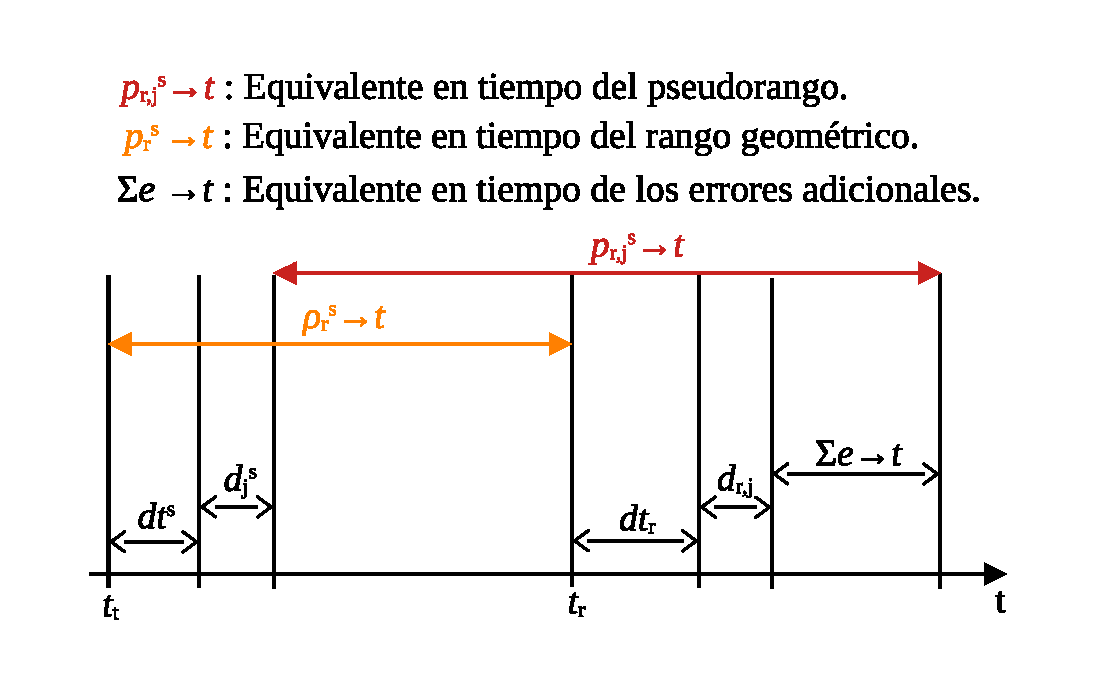
\includegraphics[width=0.8\textwidth]{/GNSS/observables.eps}
    \caption{Medición de pseudorango en base a tiempos.}
    \label{fig:observables}
\end{figure}
	
\subsection{Medición de fase de portadora}%19.1.2 en el handbook.
	La medición de fase de portadora se realiza en el lazo de enganche de fase (PLL por sus siglas en inglés), midiendo el desfasaje que existe entre la portadora recibida y la portadora réplica generada internamente en el receptor. Se mide la fase de la componente de portadora pura, es decir, sin el código PRN ni el mensaje de navegación. La medición natural es la cantidad de ciclos de portadora que transcurrieron entre la transmisión y la recepeción de la señal, que cabe aclarar que no se obtiene contando ciclos. Este valor es estimado por el receptor como el resultado de la integración del \textit{doppler} de portadora, por esto también suele ser referido como rango \textit{doppler} acumulado. Una vez que se cuenta con una medida de cantidad de ciclos de portadora en el tiempo de viaje de la señal, el rango se obtiene multiplicando por la longitud de onda. Esta longitud estará en el rango de 19 cm a 25 cm, el valor más chico corresponde a la señal L1 y la mayor a L2. Esta longitud de onda pequeña trae ventajas a la medición en términos de precisión, se logra una precisión mucho más alta que con la medición de pseudorango. Sin embargo, en este enfoque no es posible salvar la ambigüedad haciendo uso del mensaje de navegación ya que se pierde la señal modulada en la portadora. Es por esta razón que existe un numero entero de longitudes de onda presente en esta medición que se mantiene sin resolver. La ecuación de observación con medición de fase de portadora es
\begin{align}\label{ec:obs_fasedep}
	\varphi _{r,j}^s(t) = \rho_r^s(t) + \zeta_{r,j}^s(t) + c\left( \delta_{r,j}^s - \delta_j^s \right) + c\left( dt_r(t) - dt^s(t) + \delta t^{rel}(t)\right) &\\ 
	- I_{r,j}^s(t) + T_r^s(t) + \lambda_j \left( \omega_r^s(t) + N_{r,j}^s \right) + \epsilon_{r,j}^s(t)& \ . \nonumber
\end{align}
\begin{itemize}
	\item $\varphi _{r,j}^s(t)\,[m]$: Medición de fase de portadora entre el usuario y el satélite obtenido con la ecuación de observación, siendo $j$ el identificador de las señales del mismo satélite.
	\item $\rho_r^s(t)$, $dt_r(t)$, $dt^s(t)$, $\delta t^{rel}(t)$, $I_{r,j}^s(t)$, $T_r^s(t)$: Equivalentes a los términos en la Ecuación \eqref{ec:obs_pseudorango}.
	\item $\zeta_{r,j}^s\,[m]$: Término de corrección debido a sesgos en los centros de fase de las antenas transmisora y receptora.
	\item $\delta_{r,j}$, $\delta_j^s\,[s]$: Retardos instrumentales o de hardware en el receptor y en el satélite, respectivamente.
	\item $\lambda_j\,[m]$: Longitud de onda a la frecuencia de la señal j-ésima.
	\item $\omega_r^s(t)\,[ciclos]$: Corrección de \textit{wind-up} de fase. Corresponde a cambios en la fase medida en caso de rotación de las antenas.
	\item $N_{r,j}^s\,[ciclos]$: El número entero de ciclos de la portadora presentes en la medición, es la ambiguedad que queda sin resolver.
	\item $\epsilon_{r,j}^s(t)$: Errores adicionales, tales como multicamino y por ruido térmico en el receptor.
\end{itemize}
Cabe destacar que los términos que representan los mismos fenómenos que en la Ecuación \eqref{ec:obs_pseudorango} pero tienen distintos símbolos, es debido a que tienen distinta naturaleza. Y se puede realizar un gráfico equivalente a la Fig.~\ref{fig:observables} pero para la ecuación de observación de fase de portadora.

	Los términos desconocidos son obtenidos al resolver el sistema de ecuaciones linealizadas ya mencionado, sin embargo, se pueden observar múltiples épocas y de esta manera realizar una estimación de estos parámetros. No solo se estiman los términos correspondientes a los errores de rango, si no también se incluye la ambigüedad de fase de portadora. En principio, todos los términos desconocidos de la Ecuación \eqref{ec:obs_fasedep} son estimados.
	
	Una forma de tener control en el valor de las ambigüedades que observamos en la Ecuación \eqref{ec:obs_fasedep} es alineando el inicio de la integración del \textit{doppler} con el correpondiente pseudorango. De esta manera aseguramos no tener un valor de ambigüedades que aparte considerablemente la medición de fase de la medición de pseudorango, aunque de igual manera se mantendrán las ambigüedades en la medición.
\section{Errores}\label{sec:errores}
	Es de particular interés para este trabajo analizar la naturaleza de los términos de error que están involucrados en las Ecuaciones \eqref{ec:obs_pseudorango} y \eqref{ec:obs_fasedep}. Será de gran utilidad a la hora de trabajar con observaciones en diferencias. 
\subsection*{Error en el reloj del satélite y usuario}
	El término que hace referencia a este fenómeno del lado del satélite es $dt^s(t)$. Es necesario aclarar que los satélites GPS cuentan con relojes atómicos de elevada estabilidad, por lo que los errores son principalmente debido a sesgos entre el sistema de tiempo GPS y el tiempo propio del satélite. El tiempo del sistema está referenciado al tiempo UTC (USNO)~\cite{utc}. El segmento de tierra se encarga de enviar varias veces por hora las correcciones necesarias para disminuir este error en los satélites GPS, haciendo que la diferencia entre el tiempo del satélite y la del sistema GPS sea menor a 1\,$\mu s$. Además, cada satélite transmite parámetros para que el usuario pueda corregir la diferencia de tiempo que queda remanente entre el tiempo del satelite y el tiempo del sistema. La actualización de estos parámetros se realiza diariamente. Se transmiten un coeficiente para corregir el sesgo de reloj, la deriva de reloj y la deriva de frecuencia o envejecimiento, $a_{f0}$, $a_{f1}$, $a_{f2}$ respectivamente. Y con ellos se obtiene 
\begin{equation}\label{ec:corr_satclk}
	dt^s(t) = a_{f0} + a_{f1}(t-t_{oc}) + a_{f2}(t-t_{oc})^2 \ .
\end{equation}
	Se define una curva usada para corregir el tiempo del satélite, de manera que $t_{oc}$ es el tiempo de referencia para el cual la curva es válida.
	
	En cuanto al error del usuario, denotado $dt_r(t)$, es una medida de desincronización del reloj del usuario con el tiempo del sistema GPS.
\subsection*{Retardos instrumentales en satélite y usuario}
	Corresponden a sesgos en la etapa de procesamiento, ya sea analógico o digital. El término dependiente del satélite ($d_j^s$), es causado por diferencias de retardo en el camino analógico y digital de la unidad de generación de la señal y de la antena, que no son iguales para las distintas señales. Este término es asumido igual para todos los receptores que se encuentren siguiendo a la misma señal. La contribución asignada al usuario ($d_{r,j}$), es causado por diferencias de camino de la señal desde la antena a la etapa de correlación. Son asumidos iguales para todas las señales del mismo tipo siempre y cuando sean recibidas por el mismo usuario.
	
	 Cabe destacar que la parte principal de esta componente de sesgo no corresponde a la sección analógica del receptor, sino a la cadena de procesamiento digital de la señal (DSP por sus siglas en inglés)~\cite{handbook}(19.6.2). De manera que son sesgos que se pueden eliminar mediante una correcta calibración del receptor.
\subsection*{Sesgo en el centro de fase de la antena}
	Al tratar con la posición del satélite o del usuario se termina considerando la ubicación de la antena transmisora y receptora, respectivamente. Para ser más precisos, el centro de fase de ambas antenas, y el mismo puede no mantenerse fijo. Tiene influencia en especial para aplicaciones de alta precisión, ya que considerar que todas las señales llegan a un mismo punto deja de ser valido dependiendo de la dirección con la que inciden las señales a la antena y la frecuencia. Este es otro efecto que puede ser desafectado mediante calibración.
	 
\subsection*{Sesgo debido al efecto relativista}
	Este término aparece como $\delta t^{rel}(t)$ en la ecuación de observación. El reloj del satélite sufre desviaciones en frecuencia respecto a uno que se encuentra en tierra, debido al movimiento del satélite y los cambios en el potencial gravitatorio. Para compensar este efecto (atribuido a la relatividad especial y general) los relojes no trabajan exactamente a la frecuencia necesaria para generar las señales L1 y L2, sino que generan una frecuencia levemente menor. En lugar de considerar la frecuencia $f_0 = 10.23$\,MHz para generar las frecuencias L1 y L2, se configura $f_0 = 10.22999999543$\,MHz. De esta manera, cualquier usuario en tierra recibe la señal compuesta con los efectos relativistas, y observa la señal sin desviación de la frecuencia esperada. Sin embargo, esta corrección efectuada en el satélite, no corrige todo tipo de error ya que las órbitas de los satélites GPS no son perfectamente circulares. Se agrega entonces una contribución al corrimiento en frecuencia debido a la excentricidad no nula de la órbita y el mismo puede ser calculado como
\begin{equation}
	\delta t^{rel}_{clk}(t) = -\dfrac{2}{c_0^2}\sqrt{a\mu}e\sin(E) \ .
\end{equation}
	Donde $a$ es la longitud del semieje mayor de la órbita, $e$ la excentricidad de la órbita, $\mu$ la constante gravitacional geocéntrica y $E$ la anomalía excéntrica del satélite. Se puede acotar este termino ya que la excentricidad máxima permitida para las órbitas GPS es de 0.02, resultando en 45\,ns, lo que equivale a 13.5\,m.
	
	 Por otro lado, existe una contribución debido al efecto \textit{Shapiro}, un retardo en la señal debido al campo gravitacional de la tierra. El mismo tiene un valor máximo de 60\,ps para un usuario en la tierra, equivalente a 2\,cm considerando satélites MEO como lo son las constelaciones GNSS. Todas estas contribuciones son las que conforman el término ya mencionado en la ecuación de observación.
	 
%\begin{figure}
%    \centering
%    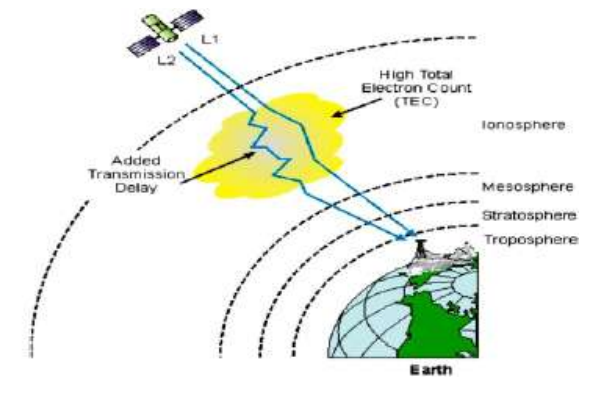
\includegraphics[width=0.6\textwidth]{GNSS/atmosferic_effects.png}
%    \caption{Efectos de la atmósfera en la propagación de la señal.}
%    \label{fig:atm_effects}
%\end{figure}
	 
\subsection*{Retardo ionosférico}
	Uno de los dos efectos atmosféricos presentes en la medición de las señales GPS es el debido a la ionósfera. El hecho de que la ionósfera sea un medio dispersivo genera diferentes retardos a las distintas componentes en frecuencia de la señal, en particular la señal se atrasa frente a la fase de portadora, efecto conocido como divergencia ionosférica. Las variaciones en el índice de refracción que sufre la ionósfera se deben a cambios que existen en el contenido total de electrones (TEC por sus siglas en inglés); estos cambios se comportan con una dinámica lenta por lo que realizar mediciones en una suficiente cantidad de épocas puede proveer una buena estimación de la corrección a realizar. Por otro lado, se pueden aplicar mediciones a doble frecuencia para aprovechar la dependencia del retardo con la misma, y así estimar la corrección. 
	
	En las expresiones de observación de las Ecuaciones \eqref{ec:obs_pseudorango} y \eqref{ec:obs_fasedep} el retardo ionosférico tiene distinto signo. Esto se debe al hecho de que es un medio dispersivo y dado que la fase y el código no viajan a la misma velocidad ambos son afectados por un índice de refraccion distinto. El correspondiente a la envolvente se puede aproximar a primer órden como 
\begin{equation}
	n_g \approx 1 + \dfrac{40.3n_e}{f^2} \ ,
\end{equation}
	con $n_e$ la densidad de electrones. En el caso del índice aproximado para la fase de portadora se obtiene
\begin{equation}
	n_p \approx 1 - \dfrac{40.3n_e}{f^2} \ .
\end{equation}
	Calculando los retardos de grupo y fase como 
\begin{equation}
	\Delta\uptau_{g,p} = \dfrac{1}{c}\int\left( n_{g,p}(l) - 1 \right)dl = \pm \dfrac{40.3\cdot TEC}{cf^2} \ ,
\end{equation}
	se puede ver como para la medición de fase de portadora el retardo ionosférico resulta con signo opuesto que para el pseudorango. 
	
	Debido a esta dependencia con la frecuencia del retardo producido por la ionósfera, que incluso puede ser predecida, es que los sistemas GNSS transmiten señales en distintas frecuencias. De esta manera un receptor recibiendo señales en múltiples frecuencias puede compensar estos efectos en las mediciones.
	
	
\subsection*{Retardo troposférico}
	El retardo debido a la tropósfera está asociado a las irregularidades que existen en el índice de refracción de la misma. Este fenómeno es un efecto que afecta a la señal en la última etapa del camino que recorre desde el satélite hasta el usuario, si el mismo se encuentra en tierra. No se observan variaciones a gran escala del índice de refracción, por lo que la tropósfera es un medio no dispersivo en la banda de GPS (banda L). Se puede separar en dos componentes, la componente seca es predominante (se lleva un 90\% de la contribución total de este efecto) y tiene alto grado de predictibilidad. El otro 10\% es denominado la componente húmeda y no es tan sencillo de predecir. La separación se hace según la altura de la capa, siendo la componente seca la correspondiente a la parte inferior de la atmósfera (tropósfera) y la componente húmeda la capa superior a la tropósfera (estratósfera aunque en estas aplicaciones se consideran como un conjunto).

	Los dos términos de retardo atmosférico son altamente dependientes del ángulo de elevación que existe entre el usuario y el satélite interceptado. Esto es evidente debido a que la cantidad de atmósfera que atraviesa la señal es menor cerca del cenit y mayor para ángulos de elevación pequeños. Para los fines del posicionamiento diferencial en el que se centra este trabajo, es importante remarcar que las características de la ionósfera y tropósfera son dependientes de la zona, debido a los efectos climáticos. Este aspecto será de gran utilidad a la hora de analizar combinación de múltiples mediciones entre receptores con distinta ubicación.
\subsection*{Errores adicionales}
	Los errores adicionales pueden provenir de distintas fuentes o tener naturalezas completamente diferentes, pero de igual manera se juntan todas estas contribuciones en un término adicional. En principio este término contiene el ruido térmico propio del receptor y el de las etapas previas al mismo. Además de ruidos de fuentes externas que pueden sumarse a la señal. No es posible desafectar este término debido a su naturaleza aleatoria, y será parte de la estimación en las mediciones de pseudorango y fase de portadora. Otro efecto incluido en este termino es el de los errores debido al multicamino, que no se pueden considerar de naturaleza aleatoria ya que dependen de la geometría de la constelación GNSS en esa época, receptor y el medio en el cual está inserto. La razón por la que no se pueden eliminar mediante filtrado pasa bajos es porque no tienen media nula~\cite{handbook}. 
	
\section{Determinación de la posición}
	Para determinar la posición, el usuario debe medir los rangos a cada satélite y resolver su posición mediante la combinación de estas. Para lograr la solución de posición se utilizan distintas observaciones, cuatro mediciones son necesarias para poder obtener la solución puntual. Pero también se puede utilizar información redundante para obtener una solución más confiable, pudiendo aplicar algún tipo de estimación de mínimos cuadrados o simplemente para validar la solución obtenida. El sistema de ecuaciones a resolver parte de plantear el verdadero rango entre el usuario y cada satélite como 
\begin{equation}
	\left \lVert \mathbf{s}^j - \mathbf{u} \right \rVert = \rho_r^{s,j} - c(t_u-\delta t^j)
\end{equation}
	con 
\begin{equation}
	t_u = t_r - t \ .
\end{equation}
	Siguiendo la notación como sigue
\begin{itemize}
  \item[] $\mathbf{s}^j = (x^j,y^j,z^j)$: vector de posición tridimensional del satélite j-esimo.
  \item[] $\mathbf{u} = (x_u,y_u,z_u)$: vector de posición tridimensional del usuario.
  \item[] $\rho_r^{s,j}$: pseudorango entre el usuario y el satélite j-esimo.
  \item[] $t_r$: tiempo del receptor.
  \item[] $t$: tiempo del sistema.
  \item[] $t_u$: sesgo entre el tiempo del receptor y el tiempo del sistema.
  \item[] $\delta t^j$: sesgo entre el tiempo del satélite y el tiempo del sistema.
\end{itemize}
	Las posiciones están en coordenadas ECEF~\cite{kaplan} y se puede considerar que $\delta t^j$ es nulo ya que al momento de computar el tiempo de transmisión de la señal el mismo fue corregido para estar sincronizado con el tiempo del sistema. Con esta asunción cada pseudorango resulta
\begin{equation}
	\rho_r^{s,j} = \left \lVert \mathbf{s}^j - \mathbf{u} \right \rVert + ct_u = \sqrt{(x^j-x_u)^2+(y^j-y_u)^2+(z^j-z_u)^2} + ct_u \ .
\end{equation} 
	Si se toman mediciones de múltiples satélites se obtiene un sistema de ecuaciones no lineales para resolver $\mathbf{u}$ y $t_u$. Es común en la literatura realizar una linealización en torno a una posición estimada del usuario $\hat{\mathbf{u}}$~\cite{kaplan}, para esto se definen los pseudorangos estimados como
\begin{equation}\label{ec:psrn_est}
	\hat{\rho}_r^{s,j} = \sqrt{(x^j-\hat{x}_u)^2+(y^j-\hat{y}_u)^2+(z^j-\hat{z}_u)^2} + c\hat{t}_u = \hat{r}_r^{s,j} + c\hat{t}_u \ .
\end{equation}
	Se puede observar la definición de $\hat{r}_r^{s,j}$ por simplicidad de la notación. Al linealizar $\rho_r^{s,j}$ en torno a la posición estimada $\hat{\mathbf{u}}$, es posible obtener una expresión para el pseudorango que se quiere calcular en función de \eqref{ec:psrn_est}. Esta expresión resulta
\begin{equation}
	\rho_r^{s,j} = \hat{\rho}_r^{s,j} - \dfrac{(\mathbf{s}^j - \hat{\mathbf{u}})\Delta \mathbf{u}}{\hat{r}_r^{s,j}} + c\Delta t_u \ .
\end{equation}
	El incremental de posición del usuario respecto a su posición estimada ($\Delta \mathbf{u}$) está escalado por el rango entre la posición estimada del usuario y el satélite, es decir la diferencia de los vectores posición de cada uno. Este término es dividido por la norma de este vector diferencia $\hat{r}_r^{s,j}$, por lo que resulta en un vector unitario que apunta desde la posición estimada del usuario al satélite j-ésimo. Siendo las componentes de este vector los cosenos directores del vector $(\mathbf{s}^j - \hat{\mathbf{u}})$, no es otra cosa que el vector unitario línea de vista (LOS por sus siglas en ingles). De esta manera se define
\begin{equation}\label{ec:uLOS}
	\mathbf{a}^j = \dfrac{\mathbf{s}^j-\hat{\mathbf{u}}}{\hat{r}_r^{s,j}} \ .
\end{equation}	
	El sistema de ecuaciones a resolver en función de los sesgos de los pseudorangos $\Delta\rho_r^{s,j} = \hat{\rho}_r^{s,j}-\rho_r^{s,j}$ se puede escribir como
\begin{equation}
	\Delta \boldsymbol{\rho}_r^s = \begin{bmatrix}
\Delta \rho_r^{s,1} \\
\Delta \rho_r^{s,2} \\
\vdots \\
\Delta \rho_r^{s,N} 
\end{bmatrix} = \begin{bmatrix}
\mathbf{a}^1 & 1 \\
\mathbf{a}^2 & 1 \\
\vdots & 1 \\
\mathbf{a}^N & 1 
\end{bmatrix} \begin{bmatrix}
\Delta x_u \\
\Delta y_u \\
\Delta z_u \\
-c\Delta t_u 
\end{bmatrix} = \mathbf{H}^{\scaleto{N}{4pt}}\cdot \Delta \mathbf{x}_u \ .
\end{equation}
La matriz $\mathbf{H}^{\scaleto{N}{4pt}}$ solo depende de la geometría entre los satélites en vista (o utilizados para resolver posición) y el usuario. La cantidad mínima de mediciones de pseudorango que se precisa para resolver posición y sesgo en tiempo es $N=4$; en este caso es posible hallar el vector $\Delta \mathbf{x}_u$ multiplicando por izquierda al vector de sesgos de pseudorango por la matriz $\mathbf{H}^{\scaleto{N}{4pt}}$ inversa. Si todas las mediciones de pseudorango son coherentes el sistema está unívocamente determinado. Puede interpretarse que la ubicación del usuario se resuelve con mediciones de tres satélites (en caso de que no hubiese error de tiempo alcanza con esto) y se agrega un cuarta medición para poder resolver el sesgo de reloj entre el usuario y el satélite.

	Como ya fue mencionado, se pueden usar más mediciones de las necesarias para resolver unívocamente el sistema. Con esto lo que se logra es validar la solución obtenida con mediciones de otros satélites, o incluso obtener información redundante para poder realizar una estimación de la posición. En particular, para casos donde $N>4$ la matriz $\mathbf{H}^{\scaleto{N}{4pt}}$ deja de ser cuadrada, por lo que no podemos resolver como se enunció para el caso $N=4$. En esta situación se trabaja multiplicando por izquierda por la matriz $\mathbf{H}^{\scaleto{N}{4pt}}$ transpuesta obteniendo
\begin{equation}
	\mathbf{H}^{\scaleto{N}{4pt}T} \cdot \Delta \boldsymbol{\rho}_r^s = \underbrace{\mathbf{H}^{\scaleto{N}{4pt}T} \mathbf{H}^{\scaleto{N}{4pt}}}_{4\times 4} \Delta \mathbf{x}_u \ .
\end{equation}
	De manera que se forma una matriz de $4\times 4$ a la cual se le puede obtener la inversa y así hallar la solución mediante mínimos cuadrados como 
\begin{equation}
	\mathbf{\Delta x_u} = \left(\mathbf{H}^{\scaleto{N}{4pt}T} \mathbf{H}^{\scaleto{N}{4pt}}\right)^{-1} \cdot \mathbf{H}^{\scaleto{N}{4pt}T} \cdot \Delta \boldsymbol{\rho}_r^s \ .
\end{equation}
	Cabe aclarar que si el punto de linealización esta lo suficientemente cerca de la posición verdadera del usuario, no hace falta realizar una iteración del procedimiento para obtener una solución. En cambio, si se parte de una posición estimada que no se acerca a la real, se deberá iterar utilizando como nueva posición aproximada la solución que devuelve el método. Este procedimiento es repetido hasta lograr una solución aceptable, es por esto que para obtener la solución en frío, un receptor puede demorar bastante tiempo según cual sea el grado de calidad de la información a priori que conozca de su posición.\\
	
	Con esto se plantearon las bases y conceptos principales del funcionamiento de los sistemas GNSS, siempre haciendo foco en el posicionamiento absoluto. Se detallaron los errores que están involucrados en las mediciones, dando lugar a reflexionar sobre formas de corregirlos o mitigarlos. Las mediciones de pseudorango son de utilidad para resolver la posición pero tienen grandes errores debido a que se generan en el DLL. La precisión que aportan las mediciones de fase de portadora es mucho mayor pero presentan el inconveniente de contar con ambigüedades. Sin tenerlas resueltas, lo cual no es trivial, se pierde esta ganancia en precisión. De aquí es natural continuar con el desarrollo de las mediciones en diferencias o posicionamiento relativo, que da lugar a formas de resolver estas ambigüedades y obtener soluciones órdenes de magnitud mas precisas. Para esto se aprovechan las características de los errores presentes en la medición. Por otro lado, se esboza el proceso de generación de las mediciones en el caso más general, además del procedimiento que permite obtener una solución de posición del receptor. Esto es un buen punto de partida para plantear la implementación de este proceso en un sistema embebido donde las prestaciones son limitadas y por lo tanto, también la capacidad de procesamiento.

\chapter{GNSS diferencial}\label{ch:DGNSS}
	Este capítulo presenta los conceptos del posicionamiento relativo, introduciendo la combinación de mediciones de múltiples satélites o múltiples receptores. Se desarrolla el concepto de GNSS diferencial haciendo foco en la posibilidad de resolución de ambigüedades en las mediciones de fase de portadora que quedó sin disolver en el enfoque del capítulo anterior. Además, se detallan los aspectos más importantes de la estandarización de los mensajes para la comunicación entre los receptores que trabajan en red en un enfoque de posicionamiento diferencial cinemático.
\section{Introducción}
	%Cuando se habla de precisión, es a 1 sigma? Definir eso...
	Un receptor GNSS operando sin ayuda externa puede lograr soluciones con precisión menor a las decenas de metros, incluso consiguiendo estar en el órden de los metros. Esto es debido a que se utilizan mediciones de pseudorango para obtener la solución, y como se desarrolló en el Capítulo~\ref{ch:GNSS} las mismas son más ruidosas que las mediciones de fase de portadora. En algunas aplicaciones críticas la precisión lograda no es suficiente, se precisan soluciones de posición con mayor precisión.  Para esto es necesario ayudar al receptor a obtener una solución con información externa o interna, una forma de realizar esto de manera interna es con GNSS diferencial haciendo uso de mediciones de fase. Un ejemplo del uso de información externa puede ser con sensores que obtienen parámetros inerciales del vehículo, y que el receptor GNSS utilice estos datos para mejorar su solución.
	
	Para poder utilizar las mediciones de fase de portadora es necesario de alguna manera resolver las ambigüedades en longitudes de onda que presentan las mismas. Existen métodos de resolución de ambigüedades que logran fijar su valor, los mismos se basan en formar mediciones en diferencias para poder cancelar distintas contribuciones que tiene la medición individual. Lo que se consigue con esto es aislar los términos que se quieren estimar, según cómo se diseñe la combinación de mediciones es posible cancelar los términos indeseados para contar únicamente con las ambigüedades y ruido a la hora de la estimación. Una vez resueltas las ambigüedades se puede explotar toda la utilidad de las mediciones de fase de portadora. Las mismas son equivalentes a una medición de pseudorango, pero con un error de más de dos órdenes de magnitud menor ya que se obtienen en el PLL, esto equivale a un nivel de ruido del órden de los milímetros. Esto permitiría obtener una solución de posición con una precisión de algunas decenas de centímetros o incluso menos. 
	
	 Al formar una red de receptores que pueden trabajar en conjunto es posible desafectar errores en las mediciones tales como efectos atmosféricos que son altamente dependientes de la ubicación del receptor o los receptores.	Los mismos deben comunicarse entre ellos enviando mensajes estandarizados por la Comisión Técnica de Radio para Servicios Marítimos (RTCM por sus siglas en inglés), de manera que logran obtener soluciones puntuales para cada receptor en la red y además se pueden obtener las posiciones relativas entre los mismos.

\section{Múltiples mediciones combinadas}\label{sec:multiples_mediciones}
	La acción de tomar múltiples mediciones y combinarlas para poder cancelar algunos de los términos, es de gran utilidad, y uno de los principales fundamentos para el posicionamiento diferencial en el que esta centrado este trabajo. Resulta de particular interés para poder proveer soluciones de posición más precisas, conocer los términos de error presentes en las ecuaciones de observación (Sección~\ref{sec:errores}). Para esto se aprovecha la correlación espacial y temporal que existe entre algunos de estos fenómenos para las distintas mediciones, ya sea modificando la geometría del problema, u observando en múltiples épocas.
	
	Las múltiples mediciones pueden hacer uso de señales de múltiples satélites con un receptor único o de una única señal recibida por múltiples receptores. En caso de contar con mediciones que no hayan sido tomadas en el mismo instante, el receptor podría propagar las mismas de manera que queden alineadas a una época común. Pero para aplicaciones de precisión como las que se plantean con este enfoque no es conveniente ya que un el desplazamiento de un satélite GNSS es muy grande incluso en pequeños intervalos de tiempo. Para poner magnitudes, por ejemplo, en un periodo de 1 segundo los satélites se desplazan casi 4\,km.
\subsection{Simples diferencias}\label{sec:SD}
	Las observaciones combinadas de simples diferencias entre receptores (BRSD por sus siglas en inglés) consisten en la diferencia de observaciones de un único satélite, usando dos receptores distintos (Fig.~\ref{fig:BRSD}). También se puede realizar la diferencia de observaciones de dos señales (satélites) en el mismo receptor (BSSD por sus siglas en inglés), la cual se denomina simples diferencias entre satélites (Fig.~\ref{fig:BSSD}). Cabe destacar que las diferencias tomadas aquí son denominadas simples pues consisten en una medición de rango entre un usuario y un satélite, el rango se puede formar con medición de pseudorango o \textit{doppler} acumulado de portadora. Existen enfoques donde las mediciones que son diferenciadas son observables combinados, es decir, una combinación lineal de pseudorangos y mediciones de fase de distintas señales, no pudiendo llamarlas observaciones simples.

	La nomenclatura correspondiente a cada medición se da con el operador $\nabla$ para simples diferencias entre satélites y $\Delta$ cuando es entre receptores. Además se agregan índices para poder identificar a los receptores y satélites. En el superíndice se indica al satélite (o par de satélites diferenciados) y en el subíndice se indica al receptor (o par de receptores diferenciados).

\begin{figure}
    \begin{subfigure}{.49\textwidth}
    \centering
    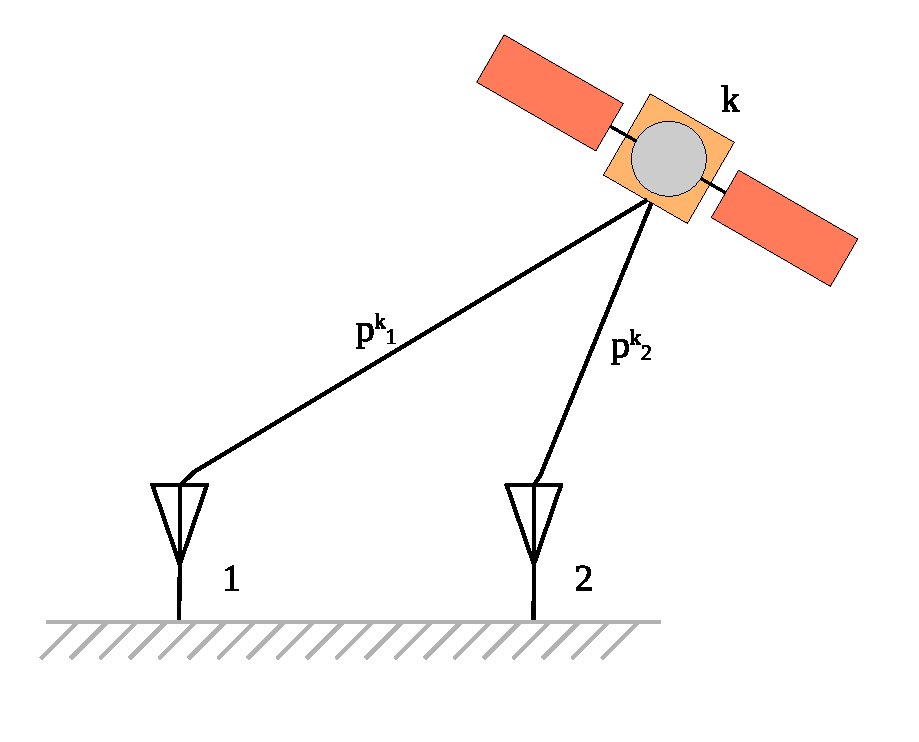
\includegraphics[width=1\textwidth]{/DGNSS/BRSD.eps}
    \caption{Diferencia entre receptores con un único satélite (BRSD).}
    \label{fig:BRSD}
    \end{subfigure}
    \begin{subfigure}{.49\textwidth}
      \centering
      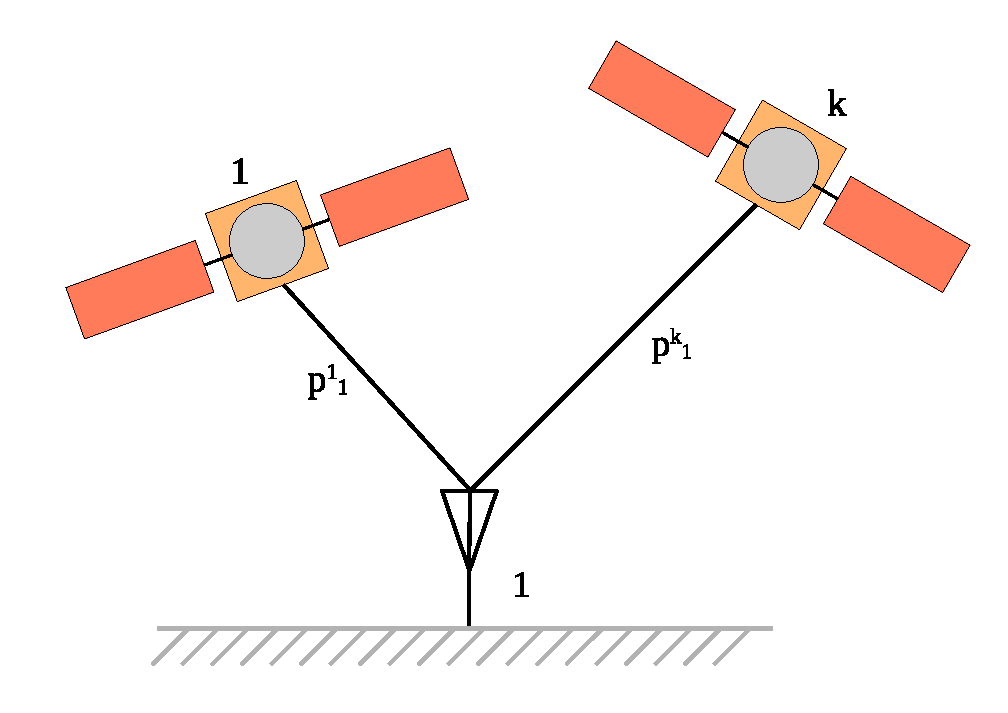
\includegraphics[width=1\textwidth]{/DGNSS/BSSD.eps}
      \caption{Diferencia entre satélites con un único receptor (BSSD).}
      \label{fig:BSSD}
    \end{subfigure}
    \caption{Esquema del armado de combinación de simples diferencias.}
    \label{fig:SimpleDiff}
\end{figure}
\subsubsection{Entre receptores}
	El pseudorango resultante de la BRSD es
\begin{align}\label{ec:BRSD_pr}
	\Delta p_{12}^k &= p_2^k - p_1^k = \rho_{12}^k +cd_{12}^k + \xi_{12}^k + c\left( dt_{12} + \delta t_{stc,12}^{rel,k} \right) + I_{12}^k(bl) + T_{12}^k(bl) + e_{12}^k \ .
\end{align}
	La fase de portadora que se forma es
\begin{align}\label{ec:BRSD_fdp}
	\Delta \varphi_{12}^k = \varphi_2^k - \varphi_1^k = \rho_{12}^k + c\left( dt_{12} + \delta t_{stc,12}^{rel,k} \right) + c\delta_{12}^k + \zeta_{12}^k - I_{12}^k(bl) + T_{12}^k(bl) &\\ + \lambda \left( \omega_{12}^k + N_{12}^k \right) + \epsilon_{12}^k & \ . \nonumber
\end{align}
	Comparando con las Ecuaciones \eqref{ec:obs_pseudorango} y \eqref{ec:obs_fasedep} se puede observar cómo se cancelan los términos que son compartidos, tales como el retardo instrumental del satélite y el sesgo en el reloj del satélite. Se conserva el término de retardo de instrumental diferencial en el receptor, debido a que solo podría cancelarse en caso de que ambos receptores cuenten con etapas de correladores y \textit{front-end} idénticos.
	
	 Por otro lado, los términos correspondientes a los retardos atmosféricos pasan a ser dependientes de la línea de base entre ambos receptores. Esto se debe a la correlación espacial que tienen estos fenómenos, cuanto menor sea la línea de base se puede considerar que estos términos son eliminados debido a que la señal atraviesa fragmentos de la atmósfera con similares características. Si bien son conservados, para líneas bases pequeñas comparadas con la distancia a los satélites pueden ser despreciados frente a errores de multicamino y propios del ruido del receptor.
	
	En la medición de fase de portadora en simples diferencias se agregan el término de corrección de \textit{wind-up} de fase y de ambigüedad entera de fase, ambos diferenciales. En general, para aplicaciones en Tierra con línea base no muy grande el que se menciona primero puede ser despreciado, debido a que las antenas están apuntando hacia arriba. En cambio, en aplicaciones donde los receptores se encuentran en vehículos espaciales esto dejaría de ser posible debido a diferencias de altura entre los mismos o por las líneas base más grandes que se presentan.
	
\subsubsection{Entre satélites}
	El pseudorango para el caso BSSD resulta
\begin{align}\label{BSSD_pr}
	\nabla p_1^{k1} = p_1^1 - p_1^k = \rho_1^{k1} + cd_1^{k1} + \xi_1^{k1} + c\left( dt^{k1} + \delta t^{rel,k1} \right) + I_1^{k1}(bl) + T_1^{k1}(bl) + e_1^{k1} \ .
\end{align}
	Y para la fase de portadora 
\begin{align}\label{BSSD_fdp}
	\nabla \varphi_1^{k1} = p_1^1 - p_1^k = \rho_1^{k1} + c\left( dt^{k1} + \delta t^{rel,k1} \right) + c\delta_1^{k1} + \zeta_1^{k1} + T_1^{k1}(bl) - I_1^{k1}(bl) &\\
	+ \lambda^1\left( \omega_1^1 + N_1^1 \right) - \lambda^k\left( \omega_1^k + N_1^k \right) + \epsilon_1^{k1}& \ . \nonumber
\end{align}

	En este caso los términos que se cancelarán son los compartidos debido a que se utiliza un único receptor. En particular, el sesgo de reloj debido al efecto relativista es cancelado tanto como el sesgo de reloj del receptor. En cuanto al retardo instrumental solo podremos indicar que el mismo se cancela si se utilizó la misma señal de ambos satélites. Esto es debido a que el retardo que corresponde a la parte analógica esta dominado por el retardo inherente a los filtros pasa banda en la etapa de RF del receptor. Como estos filtros no son iguales para todas las señales, entonces no se puede decir que para distintas señales se cancelan los retardos, también dejando en evidencia que estos retardos son propios de cada receptor~\cite{psiakis}.
	
	En definitiva, se mantiene el retardo instrumental diferencial de los satélites. Los efectos atmosféricos pueden estar correlacionados o no, según si los satélites adquiridos se encuentran en posiciones cercanas o no. Como esta situación no resulta común y en principio se puede adquirir cualquier par de satélites, se considera para el caso general que los retardos debido a los efectos atmosféricos se mantienen.
\subsection{Dobles diferencias}\label{sec:DD}
	Las mediciones en dobles diferencias (DD de aquí en más) se construyen mediante la diferenciación de dos simples diferencias, se pueden diferenciar dos mediciones BRSD con dos satélites distintos o dos mediciones BSSD con dos receptores distintos. Es evidente que será necesario contar con disponibilidad de un par de receptores y un par de satélites en vista para ambos receptores (ver Fig.~\ref{fig:DD}). Este tipo de mediciones son de particular interés ya que logran cancelar otros términos que las mediciones de simples diferencias detalladas en la Sección~\ref{sec:SD} no lograban. La notación adoptada para las mediciones de dobles diferencias es $\Delta \nabla p_{12}^{k1}$ en el caso de pseudorango y para fase de portadora resulta equivalente. Si bien se diferencian dos BRSD, cada una con un satélite distinto, esto equivale a 
\begin{align}
	\Delta \nabla (\cdot)_{12}^{k1} = \Delta (\cdot)_{12}^1 - \Delta (\cdot)_{12}^k = &\Bigl[ (\cdot)_2^1 - (\cdot)_1^1 \Bigr] - \Bigl[ (\cdot)_2^k - (\cdot)_1^k \Bigr] \\ 
	= & \Bigl[ (\cdot)_2^1 - (\cdot)_2^k \Bigr] - \Bigl[ (\cdot)_1^1 - (\cdot)_1^k \Bigr] = \nabla(\cdot)_2^{k1} - \nabla(\cdot)_1^{k1} \ .  \nonumber
\end{align}
	Por lo que podemos pensar a las dobles diferencias como una BRSD y una BSSD, por eso es que obtienen la ganancia respecto a cancelación de términos comparadas con unas SD. De manera que este nuevo operador es una combinación de los operadores vistos en la Sección~\ref{sec:SD}.
\begin{figure}
    \centering
    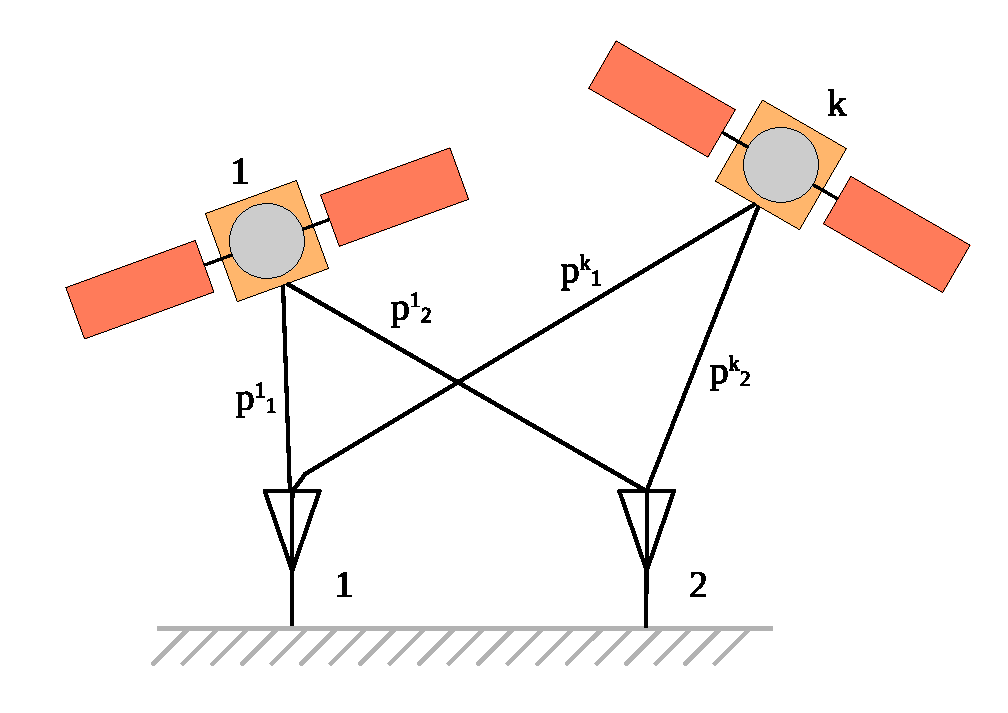
\includegraphics[width=0.7\textwidth]{/DGNSS/DD.eps}
    \caption{Configuración de receptores y satélites necesaria para dobles diferencias (DD).}
    \label{fig:DD}
\end{figure}
	La medición en DD con dos mediciones BRSD para pseudorango resulta
\begin{equation}\label{ec:DD_pr}
	\Delta \nabla p_{12}^{k1} = \Delta p_{12}^1 - \Delta p_{12}^k = \rho_{12}^{k1} + \xi_{12}^{k1} + T_{12}^{k1}(bl) + I_{12}^{k1}(bl) + e_{12}^{k1} \ .
\end{equation}
	En el caso de fase de portadora se obtiene
\begin{align}\label{ec:DD_fdp}
	\varphi_{12}^{k1} = \rho_{12}^{k1} + \zeta_{12}^{k1} + T_{12}^{k1}(bl) - I_{12}^{k1}(bl)	+\lambda \left( \omega_{12}^{k1} + N_{12}^{k1}\right) + \epsilon_{12}^{k1} \ .
\end{align}
	En estas mediciones se logra cancelar los sesgos de reloj del receptor que no se habían cancelado en las Ecuaciones \eqref{ec:BRSD_pr} y \eqref{ec:BRSD_fdp}. Además el término diferencial de corrección relativista es eliminado ya que son iguales para todas las mediciones de BRSD sin importar qué satélite se tome. Los retardos instrumentales diferenciales entre los receptores se cancelan al utilizar el mismo par de receptores, en caso de estos receptores estén diseñados de manera correcta y se pueda considerar que los retardos se compensan para las distintas frecuencias. Los términos de retardo atmosférico se mantendrán siempre y cuando no haya correlación entre las mediciones, es por esto que es explicita la dependencia de los mismo con la longitud de la línea de base. Ya se puede considerar que para SD estos términos pueden ser despreciados frente a los errores, es decir que con esta combinación tenemos más argumentos para poder hacerlo. Para líneas de base no muy grandes estos términos son tan pequeños que no se tienen en cuenta, esto es valido ya que se combinaron observaciones BRSD para dos satélites distintos por lo que el remanente es prácticamente nulo.

\subsection{Triples diferencias}
	Además de la correlación espacial que tienen los fenómenos que todavía no se han cancelado completamente, los mismos cuentan con una correlación temporal que no se ha podido tener en cuenta todavía. Esto se debe a que las mediciones en SD y DD, todas son haciendo diferencias de observaciones en la misma época. Las mediciones en triples diferencias se realizan mediante dos DD pero en distintas épocas, esto permite sacar provecho de la dinámica lenta que tienen las efectos atmosféricos. La notación tomada para identificar estas mediciones es $\partial p_{12}^{k1}$.
	
	La medición en triples diferencias de pseudorango y fase de portadora resulta
\begin{align}
	\partial p_{12}^{k1} = p_{12}^{k1}(t_i) - p_{12}^{k1}(t_{i-1}) = \partial\rho_{12}^{k1} + \partial\xi_{12}^{k1} + \partial T_{12}^{k1}(\Delta t,bl) + \partial I_{12}^{k1}(\Delta t,bl) + \partial e_{12}^{k1} \ ,
\end{align}
\begin{align}
	\partial \varphi_{12}^{k1} = p_{12}^{k1}(t_i) - p_{12}^{k1}(t_{i-1}) = \partial\rho_{12}^{k1} + \partial\zeta_{12}^{k1} + \partial T_{12}^{k1}(\Delta t,bl) - \partial I_{12}^{k1}(\Delta t,bl) + \partial \epsilon_{12}^{k1} + \partial\omega_{12}^{k1}\ .
\end{align}
	Además de los términos que ya no estaban presentes en las DD y lo que se han reducido las contribuciones atmosféricas, según qué tan grande es la diferencia de épocas tomada $\Delta t = t_{i-1}-t_i$ en comparación con la dinámica del fenómeno, podremos despreciar aún más estos términos. Es evidente que si la correlación espacial presente en los términos no fue suficiente como para despreciarlos, con un correcto diseño en este enfoque se consigue despreciarlos definitivamente.
\subsection{Línea de base nula}
	Este enfoque para armar las observaciones puede ser utilizado ya sea con simples diferencias tanto como con dobles diferencias. Es un caso particular de las ya mencionadas donde se utiliza la misma antena para ambos receptores, se divide la señal y cada receptor hace sus mediciones como se observa en la Fig.~\ref{fig:ZB}. Esto consigue que la correlación espacial sea completa debido a que la línea de base nula implica que ambos receptores usan la misma antena, por lo que la señal recorre el mismo camino para ambos, es decir, es afectada por los mismos fenómenos. Resulta de gran utilidad para la calibración de los receptores por los resultados que se obtienen. Pero en principio como geometría para posicionamiento diferencial no tiene utilidad ya que ambos receptores tienen la misma ubicación.
	
\begin{figure}
    \centering
    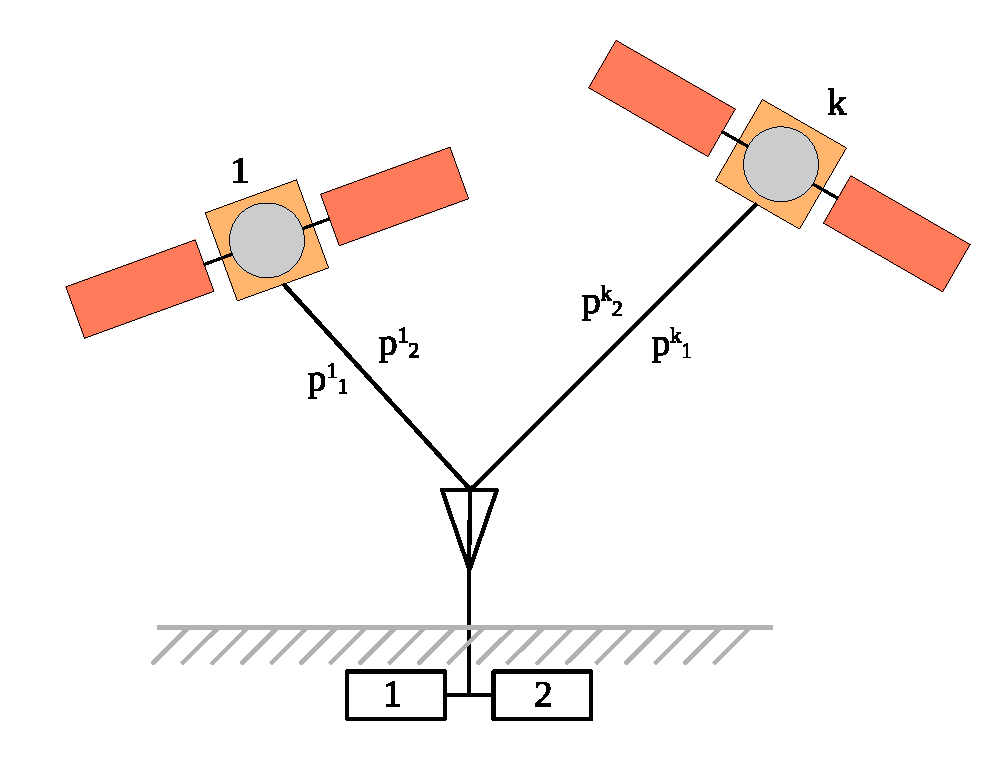
\includegraphics[width=0.7\textwidth]{/DGNSS/ZB.eps}
    \caption{Configuración con línea de base nula.}
    \label{fig:ZB}
\end{figure}

	En el caso de las simples diferencias no tiene sentido considerar entre satélites ya que no aprovecharíamos la línea de base nula, por lo que se trabajara entre receptores. Podemos analizar los términos remanentes en la Ecuación \eqref{ec:BRSD_pr} y \eqref{ec:BRSD_fdp}. En principio se mantiene el término debido al sesgo de reloj y retardo de hardware del receptor. Si bien la antena es la misma, los receptores son independientes por lo que el retardo de reloj no tiene por qué ser igual. Incluso en un caso desfavorable los receptores podrían no estar cerca y que la división de la señal implique un camino mas largo para un receptor que para otro. Se considerará que el retardo instrumental diferencial será nulo con el mismo criterio que se detalló en las secciones anteriores. Siendo cauteloso en que el diseño de los receptores es el correcto y que los cables entre el divisor de potencia y los receptores tienen el mismo largo, podemos obviarlo. Hasta acá no hay cambios con respecto al caso de receptores con antenas separadas, excepto que el rango entre ambos receptores es nulo. El cambio sustancial aparece cuando los términos de retardos atmosféricos ya son cancelados completamente en las SD ya que el camino de la señal es el mismo para ambas mediciones. El sesgo debido al centro de fase de la antena y la corrección del \textit{wind-up} de fase es el mismo para ambos receptores ya que utilizan la misma antena, por esto su contribución diferencial desaparece. Las ecuaciones resultantes son
\begin{align}
	p_{12,ZB}^k =& cdt_{12} + e_{12}^{k} \ , \\
	\varphi_{12,ZB}^k =& cdt_{12} + \lambda N_{12}^k + \epsilon_{12}^k \ .
\end{align}
	
	Al momento de tomar DD ya hay muchos términos que fueron cancelados de antemano, pero sigue resultando en ganancia ya que se cancela el sesgo de reloj entre los dos receptores que es común en ambas mediciones diferenciales. Las mediciones en DD para fase de portadora resultan
%\begin{equation}
%	p_{12,ZB}^{k1} = cd_{12}^{k1} + e_{12}^{k1}
%\end{equation}	
%	para pseudorango y para fase de portadora se obtiene
\begin{equation}
	\varphi_{12,ZB}^{k1} = \lambda N_{12}^{k1} + \epsilon_{12}^{k1} \ .
\end{equation}
	No se especifica cómo resulta la DD para pseudorango ya que al considerar que el retardo instrumental se cancela solo tendremos errores aleatorios. En estos errores solo queda remanente el ruido ya que la contribución multicamino es cancelada en BRSD pues el angulo de incidencia de la señal es el mismo para ambos receptores, es decir, tienen los mismo rebotes, por lo tanto multicamino.
\sectionmark{Resolución de ambigüedades}
\section{Resolución de ambigüedades en mediciones de fase de portadora}\label{sec:amb_res}
%Checkear que hay mucho "de esta manera"...
	Poder resolver las ambigüedades de fase como números enteros es una cuestión clave para enfoques de posicionamiento de alta precisión. Una vez resueltas estas ambigüedades es posible utilizar las mediciones de fase como rangos con gran precisión. Este mecanismo se basa en la inferencia conjunta de parámetros enteros y reales, ya que además de estimar las ambigüedades enteras existen contribuciones reales debido al rango y distintos retardos en la señal aparte del ruido. Como se desarrollo en la Sección~\ref{sec:multiples_mediciones}, se pueden cancelar términos de las ecuaciones de observación realizando mediciones combinadas en diferencias. De esta manera se mostró que es posible aislar el término correspondiente al número entero de longitudes de onda de ambigüedad en la medición, hasta dejarlo solo en presencia de ruido en el caso de las dobles diferencias. Es valido considerar que se mantienen enteras ya que la diferencia de dos números enteros lo sigue siendo. De esta manera es posible sacar provecho de la restricción y acotar el conjunto de soluciones posibles a la estimación a un conjunto de enteros. Es parte del diseño del algoritmo elegir de manera adecuada el conjunto de potenciales soluciones, de modo que el valor correcto se encuentre dentro del mismo pero que no sea lo suficientemente extenso como para que la búsqueda dentro del conjunto lleve mucho procesamiento.
	
	Los esquemas más comunes pueden dividir el procedimiento en tres etapas, que no necesariamente podrían ser todas alcanzadas durante la ejecución del algoritmo. Las mismas se dividen en el tipo de solución buscada y encontrada, cuando la ambigüedad estimada es flotante, cuando la misma es entera y por último cuando las ambigüedades fueron fijadas.
\begin{itemize}
	\item Solución flotante
	
	Para comenzar con la estimación se debe quitar la restricción de que los valores estimados son enteros. Aquí se realiza una estimación de mínimos cuadrados convencional obteniéndose el conjunto de soluciones con su matriz de covarianza.
	\item Solución entera
	
	Aquí se vuelve a restringir las soluciones a valores enteros, existen distintos métodos de restricción tales como redondeo al entero más cercano o mínimos cuadrados enteros (ILS por sus siglas en inglés).
	\item Solución fija
	
	Cuando la solución entera obtenida en la etapa previa es aceptable se procede a fijar estos valores de ambigüedades, de manera que se pueda reajustar el estimador flotante con la diferencia entre el valor fijado y el valor flotante. Es decir, buscar el valor entero en un entorno cercano a la solución flotante. La calidad de solución que se obtiene al alcanzar el estado fijado está en el órden de la precisión de las mediciones de fase, siempre que se considere alta la probabilidad de que el valor fijado sea el correcto.
\end{itemize}
	
	Es evidente que para poder llegar a fijar las ambigüedades es necesario tomar muestras en múltiples épocas, donde el tiempo para llegar a este punto es dependiente de la calidad de las mediciones y de lo restrictivo que sea el algoritmo a la hora de la estimación. Lo desarrollado en esta sección introduce conceptualmente la resolución de ambigüedades en mediciones GNSS y simplemente a modo informativo se mencionan algoritmos que implementan lo aquí desarrollado. El algoritmo que mayor popularidad tiene actualmente es un enfoque de descorrelación de ambigüedades mediante mínimos cuadrados (LAMBDA por sus siglas en inglés), el mismo es utilizado en distintas aplicaciones tales como el posicionamiento de red global, vuelos satelitales en formación o teledetección por radar interferométrico de apertura sintética (InSAR). En el lugar de trabajo donde se llevó a cabo este trabajo fue desarrollado otro algoritmo con un enfoque  bayesiano de resolución de ambigüedades (BART por sus siglas en inglés)~\cite{bart}.

\section{Real Time Kinematics}
	La verdadera ganancia del posicionamiento relativo surge de poder obtener soluciones haciendo uso de mediciones de fase. GNSS diferencial no solo consiste en posicionamiento diferencial si no también en la resolución de las ambigüedades explicada en la sección anterior (\ref{sec:amb_res}). Se denomina cinemática de tiempo real (RTK por sus siglas en inglés), por considerar que los receptores que trabajan en conjunto han podido resolver y fijar las ambigüedades en tiempo real para utilizar las mediciones de fase con alta precisión. Si bien el caso general está especificado para receptores en movimiento se podría pensar en situaciones con algunos receptores o incluso todos, en posiciones estáticas.

	En el caso de contar con dos receptores, es natural denominar a uno como base y a otro como rover (del inglés de receptor móvil). En general la base está estática y es la que envía las correcciones al rover, aprovechando que está estática la misma podrá refinar su solución de posición haciendo uso de un modelo adecuado a la dinámica que presenta. Con esta consideración tiene sentido pensar que la base tiene una solución mucho más precisa que la del rover, por eso es quien envía las correcciones para que el rover (en movimiento o no) pueda obtener una solución de posición basada en mediciones de fase. Incluso podrían agregarse varias bases y rovers, obteniendo una red RTK. De lo desarrollado aquí se puede ver que las bases serán los receptores que envían las correcciones y los rovers quienes las reciben y utilizan para resolver su posición mediante procesamiento diferencial de mayor precisión.

	La calidad de la resolución de las ambigüedades y por ende de la solución de posición está directamente relacionada con la geometría que presentan los receptores y los satélites al momento de la medición. Es por esto que al considerar situaciones estáticas, las cuales no tienen fija la geometría entre receptores, es más difícil para el rover lograr fijar las ambigüedades y trabajar a precisión de las mediciones de fase. Si bien la constelación de satélites GNSS está en constante movimiento, su dinámica no es lo suficientemente rápida como para considerar una geometría cambiante. Esto no quiere decir que no se puede fijar ambigüedades, simplemente le llevará más tiempo. 

	La razón por la que hablamos de cambios de geometría es porque los métodos de resolución de ambigüedades (Sección~\ref{sec:amb_res}) precisan mediciones de múltiples épocas para resolverlas. Y la diferencia entre épocas es la geometría entre los receptores y los satélites GNSS, de aquí es que tiene más sentido hablar de cambios de geometría. Volviendo al caso estático, se ve que el tiempo de resolución es mayor ya que se debe esperar periodos más largos para obtener el cambio de geometría necesario para resolver las ambigüedades. Al contar con pequeños cambios de geometría la precisión de la solución estará dominada por la precisión lograda con mediciones de pseudorango. Y en el caso límite donde se cuenta con con una única época es equivalente a resolver posición con pseudorango.

\section{Estándar RTCM v3.3}\label{sec:RTCM}
	Entre las bases y rovers trabajando en un esquema de posicionamiento relativo se envían mensajes de corrección para poder lograr el objetivo planteado para cinemática de tiempo real en la sección anterior. El enlace de comunicación para estos mensajes esta estandarizado por la Comisión Radio Técnica para Servicios Marítimos (RTCM por sus siglas en inglés). Existen múltiples versiones de este estándar, donde las actualizaciones agregan servicios y mensajes que se pueden transmitir. En sus comienzos solo estaban estandarizadas las correcciones de pseudorango, pero a partir de la versión 2.1 del estándar se agregan las correcciones a mediciones de fase. Hasta ese momento no era posible el enfoque RTK planteado anteriormente ya que sin las correcciones de fase de portadora no se lograba resolver las ambigüedades en esta medición. Si bien este trabajo está enfocado únicamente en un par de receptores (base y rover), a partir de la tercera versión del estándar se agrega la posibilidad de trabajar en redes RTK como las que ya se mencionaron. En particular se utiliza la versión del estándar RTCM 10403.3 (Versión 3.3) para servicios de GNSS diferencial~\cite{rtcm}.
	
	Desde el comienzo del trabajo se planteo que las ideas generales del mismo son aplicables a múltiples sistemas GNSS, pero que la implementación especifica y validación se han realizado sobre el sistema GPS. Por esta razón es que solo se analizarán los mensajes particulares para correcciones de pseudorango y fase de portadora en el sistema GPS. Aunque por la organización y modularización del estándar lo que se desarrolla es extrapolable a otras constelaciones GNSS, solo debiendo analizar en detalle los campos específicos de los mensajes que aquí no se tratan.
	
	En términos generales este documento cuenta con la estandarización de mensajes para los sistemas GPS, GLONASS, \textit{Galileo}, SBAS, QSZZ, \textit{BeiDou}. El rango de mensajes desde el Tipo 1 hasta 100 es reservado a mensajes experimentales, luego comienzan a partir del Tipo 1000. Aquí es donde se pueden encontrar mensajes de descripción de las antenas, descripción de las estaciones base, mensajes de observables y correcciones varias al operar en una red RTK. Cada mensaje tiene un identificador de tipo dado por el número y contiene distintos campos dentro, estos campos pueden verse repetidos entre los distintos mensajes. Se identifican mediante DFXXX (por \textit{Data Field}) y un número de tres dígitos. 
	
	Para la aplicación en la que está pensada este trabajo, donde se utiliza como base una única estación de referencia estacionaria, solo será necesario describir la misma y luego enviar esa información junto con los observables al rover (o rovers si hubieran más). Con este enfoque el rover cuenta con todos los datos para realizar el procesamiento diferencial internamente y en tiempo real.
\subsection{Formato del mensaje}\label{sec:RTCM_format}
	El formato que tomará el mensaje definirá por completo la capa de transporte de este enlace de comunicación entre receptores. Dando un formato común a todos los mensajes a transmitir se puede generalizar el proceso de codificación y decodificación de los mismos. Los mensajes tendrán un encabezado de 3 bytes, el contenido del mensaje será variable entre 0 y 1023 bytes, y por último, un pie de 3 bytes también.
	
	En principio es necesario definir un preámbulo que será utilizado por el rover para definir el comienzo de un mensaje. El rover podría estar recibiendo múltiples mensajes consecutivos, de una o varias bases, a través de la detección del preámbulo en la secuencia de bits recibidos el mismo puede identificar un nuevo mensaje. El preámbulo es una secuencia de un byte correspondiente a 0xD3 en hexadecimal. Luego del preámbulo existen seis bits reservados que en la versión utilizada del estándar se especifican en cero, pero como está sujeto a modificaciones el software del receptor no debe utilizar estos seis bits en cero para la decodificación. Los diez bits restantes se llenan con el largo del mensaje (expresado en bytes), con un rango de 0 a 1023. Un esquema de lo explicado puede verse en la Tab.~\ref{tab:RTCMformat}.
	
% Please add the following required packages to your document preamble:
% \usepackage[table,xcdraw]{xcolor}
% If you use beamer only pass "xcolor=table" option, i.e. \documentclass[xcolor=table]{beamer}
\begin{table}[]
\begin{tabular}{|c|c|c|c|c|}
\hline
\rowcolor[HTML]{C0C0C0} 
Preambulo & Reservado & \begin{tabular}[c]{@{}c@{}}Largo del \\ mensaje\end{tabular}             & \begin{tabular}[c]{@{}c@{}}Contenido \\ del mensaje\end{tabular}                   & \begin{tabular}[c]{@{}c@{}}Bits de \\ paridad\end{tabular} \\ \hline
\rowcolor[HTML]{FFFFFF} 
8 bits    & 6 bits    & 10 bits                                                                  & \begin{tabular}[c]{@{}c@{}}Largo variable (número \\ entero de bytes)\end{tabular} & 24 bits                                                    \\ \hline
\rowcolor[HTML]{FFFFFF} 
11010011  & 000000    & \begin{tabular}[c]{@{}c@{}}Largo del \\ mensaje {[}bytes{]}\end{tabular} & 0-1023 {[}bytes{]}                                                                 & CRC-24Q                                                    \\ \hline
\end{tabular}
\caption{Estructura del mensaje RTCM (versión 3.3).}
\label{tab:RTCMformat}
\end{table}
%\begin{figure}
%    \centering
%    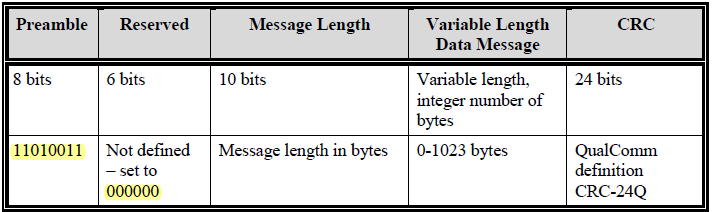
\includegraphics[width=0.8\textwidth]{/DGNSS/RTCM_format.png}
%    \caption{Estructura del mensaje RTCM (versión 3.3).}
%    \label{fig:RTCMformat}
%\end{figure}

	Luego del campo del mensaje, con largo variable, hay 3 bytes de pie que corresponden a los bits de paridad del mensaje. Corresponden a 24 bits de paridad con verificación de redundancia cíclica (CRC por sus siglas en inglés), se utiliza un código CRC de 24 bits propietario de QualComm (el mismo es llamado CRC-24Q). El mismo trabaja sobre el encabezado y el campo del mensaje, con un polinomio generador dado por 
\begin{equation}
	g(x) = \sum_{i=0}^{24}{g_ix^i} \ \ ,
\end{equation}
con 
\begin{equation*}
g_i = 1 \ \text{para} \  i = 0,1,3,4,5,6,7,10,11,14,17,18,23,24. \ \text{Y} \ g_i = 0 \ \text{en caso contrario}.
\end{equation*}

\subsection{Mensaje de la estación de referencia estacionaria}
	Existen tres mensajes para describir por completo las estaciones de referencia que actuarán como bases y sus antenas.
%Esto mensajes son 
%\begin{itemize}
%	\item Tipo 1005: Provee las coordenadas ECEF del punto de referencia de la antena (\textit{ARP} del inglés) para la base estacionaria.
%	\item Tipo 1006: Equivalente al tipo 1005 pero se agrega información sobre la altura que tiene el \textit{ARP} por encima del marcador utilizado en el proceso de obtención de la posición.
%	\item Tipo 1033: 
%\end{itemize}
	Los mismos difieren en sutilezas, por eso se desarrollarán los campos del mensaje 1005 en particular (ver Tab.~\ref{tab:Msg1005}) y luego se comentarán las diferencias que presentan los otros dos. Los mismos son genéricos para cualquier sistema GNSS. 
% Please add the following required packages to your document preamble:
% \usepackage[table,xcdraw]{xcolor}
% If you use beamer only pass "xcolor=table" option, i.e. \documentclass[xcolor=table]{beamer}
\begin{table}[]
\centering
\begin{tabular}{|l|c|}
\hline
\rowcolor[HTML]{C0C0C0} 
\multicolumn{1}{|c|}{\cellcolor[HTML]{C0C0C0}CAMPO} & \begin{tabular}[c]{@{}c@{}}Identificador\\ de campo\end{tabular} \\ \hline
Número de mensaje                                   & DF002                                                            \\ \hline
Identificador de estación de referencia             & DF003                                                            \\ \hline
Reservado                                           & DF021                                                            \\ \hline
Indicador GPS                                       & DF022                                                            \\ \hline
Indicador GLONASS                                   & DF023                                                            \\ \hline
Reservado para Indicador \textit{Galileo}                    & DF024                                                            \\ \hline
Indicador de estación de referencia                 & DF141                                                            \\ \hline
Punto de Referencia de la Antena (ARP) ECEF-X       & DF025                                                            \\ \hline
Indicador de oscilador de único receptor            & DF142                                                            \\ \hline
Reservado                                           & DF001                                                            \\ \hline
Punto de Referencia de la Antena (ARP) ECEF-Y       & DF026                                                            \\ \hline
Indicador de cuarto de ciclo                        & DF364                                                            \\ \hline
Punto de Referencia de la Antena (ARP) ECEF-Z       & DF027                                                            \\ \hline
\end{tabular}
    \caption{Campos del mensaje de estación de referencia estacionaria (1005).}
    \label{tab:Msg1005}
\end{table}

%\begin{figure}
%    \centering
%    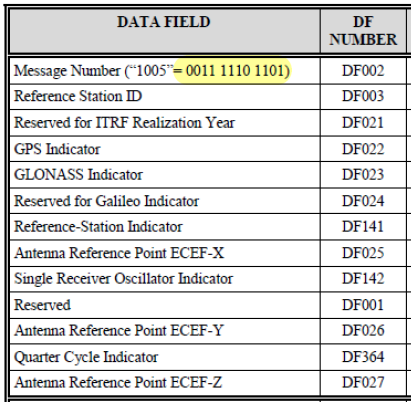
\includegraphics[width=0.6\textwidth]{/DGNSS/Msg1005.png}
%    \caption{Campos del mensaje de estación de referencia estacionaria (1005).}
%    \label{fig:Msg1005}
%\end{figure}

\begin{description}
	\item[Número de mensaje] Se especifica el número del mensaje (en este caso 1005).
	\item[Identificador de la estación de referencia] En caso de contar con múltiples bases, el rover utiliza este campo para saber de qué base proviene el mensaje.
	\item[Indicador de sistema] Está en alto si la base está enviando mensajes correspondientes al sistema en cuestión.
%	\item Indicador GLONASS: Está en alto si la base está enviando mensajes correspondientes al sistema GLONASS.
	\item[Indicador de la estación de referencia] Indica si es una estación de referencia real (física) o si es una estación computada o no física, podría ser una estación de referencia virtual computada en base a múltiples estaciones de la red.
	\item[ARP (x,y,z) en ECEF] La posición del punto de referencia de la antena de la base en coordenadas ECEF.
	\item [Indicador de oscilador de único receptor] Indica que todas las observaciones crudas enviadas en el resto de los mensajes corresponden a mediciones en el mismo instante.
	\item[Indicador de cuarto de ciclo] Indica si el fabricante del receptor que actúa como base tiene implementado un mecanismo para corregir los desfasajes de cuarto de ciclo de la fase de la portadora. Es decir que pueden asegurar que las mediciones de fase de distintas señales a una misma frecuencia están en fase y por lo tanto no presentan el desfasaje ya mencionado.
%	 Existen tres estados para este campo, el primero indica que no se conoce el estado de la corrección (corresponde a `00'), el segundo indica que se están haciendo las correcciones (corresponde a `01') y por último cuando no se hacen correcciones (corresponde a `10').
\end{description}
	
	El mensaje 1006 presenta los mismos campos que el 1005 pero como es utilizado en aplicaciones especificas de geodesia, define la altura del ARP de manera distinta. Es decir, agrega información sobre la altura del ARP respecto de un marcador del que se conoce la posición con mucha precisión. Por otro lado, el mensaje 1033 describe la antena de la estación de referencia además de dar información del tipo de receptor utilizado en la estación. Esto permite al rover generar archivos RINEX~\cite{rinex} a partir de la información recibida.
	
\subsection{Mensajes de múltiples señales}
	El estándar RTCM define los mensajes de observables dentro del rango de tipos de mensaje 1001-1004 para GPS, 1009-1012 para GLONASS. Hay mensajes particulares para cada sistema, lo cual trae complicaciones al pensar en agregar nuevos sistemas e incluso nuevas señales. Para poder generalizar los mensajes necesarios en un enfoque RTK de cualquier sistema GNSS se definen los mensajes de múltiples señales (MSM por sus siglas en inglés). Los mismos son universales para el envío de observables de cualquier sistema, lo que trae la ventaja de ya tener estandarizado los mensajes en caso de agregar disponibilidad de servicios RTK de nuevos sistemas en versiones futuras del estándar. Además de permitir generalizar según el sistema, los mismos también permiten agregar nuevas señales en las observaciones. Esto se logra compatibilizando los identificadores de señales con la tercera versión del estándar RINEX. El enfoque universal para los mensajes se logra debido a la similaridad que existe entre los observables de los sistemas operativos y los planeados.
% Please add the following required packages to your document preamble:
% \usepackage[table,xcdraw]{xcolor}
% If you use beamer only pass "xcolor=table" option, i.e. \documentclass[xcolor=table]{beamer}
\begin{table}[]
\begin{subtable}{1\linewidth}
\centering
\begin{tabular}{|l|c|c|c|c|c|c|c|}
\hline
\rowcolor[HTML]{C0C0C0} 
CAMPOS                                                                                                    & MSM1  & MSM2  & MSM3  & MSM4  & MSM5  & MSM6  & MSM7  \\ \hline
\begin{tabular}[c]{@{}l@{}}Número entero\\ de milisegundos \\ en la parte \\gruesa del rango\end{tabular} &       &       &       & DF397 & DF397 & DF397 & DF397 \\ \hline
\begin{tabular}[c]{@{}l@{}}Información\\ extendida\\ del satélite\end{tabular}                            &       &       &       &       & *     &       & *     \\ \hline
\begin{tabular}[c]{@{}l@{}}Parte gruesa\\ del rango \\ módulo 1\,ms\end{tabular}                           & DF398 & DF398 & DF398 & DF398 & DF398 & DF398 & DF398 \\ \hline
\begin{tabular}[c]{@{}l@{}}Parte gruesa\\ de la desviación\\ en frecuencia\end{tabular}                   &       &       &       &       & DF399 &       & DF399 \\ \hline
\end{tabular}
    \caption{Parte satelital. $^*$ Campo específico para cada sistema}
    \label{tab:MSMall_sat}
\end{subtable}
\vspace{0.5cm}
	
% Please add the following required packages to your document preamble:
% \usepackage[table,xcdraw]{xcolor}
% If you use beamer only pass "xcolor=table" option, i.e. \documentclass[xcolor=table]{beamer}
\begin{subtable}{1\linewidth}
\centering
\begin{tabular}{|l|c|c|c|c|c|c|c|}
\hline
\rowcolor[HTML]{C0C0C0} 
CAMPOS                                                                                         & MSM1  & MSM2  & MSM3  & MSM4  & MSM5  & MSM6      & MSM7      \\ \hline
\begin{tabular}[c]{@{}l@{}}Rangos finos\\ de \\ pseudorango\end{tabular}                       & DF400 &       & DF400 & DF400 & DF400 & DF405$^1$ & DF405$^1$ \\ \hline
\begin{tabular}[c]{@{}l@{}}Rangos finos\\ de fase de \\ portadora\end{tabular}                 &       & DF401 & DF401 & DF401 & DF401 & DF406$^1$ & DF406$^1$ \\ \hline
\begin{tabular}[c]{@{}l@{}}Tiempo de\\ enganche de \\ fase de\\ portadora\end{tabular}         &       & DF402 & DF402 & DF402 & DF402 & DF407$^1$ & DF407$^1$ \\ \hline
\begin{tabular}[c]{@{}l@{}}Indicador de \\ ambigüedades \\ de medio ciclo\end{tabular}         &       & DF420 & DF420 & DF420 & DF420 & DF420     & DF420     \\ \hline
\begin{tabular}[c]{@{}l@{}}Relación\\portadora a\\densidad\\espectral\\de ruido\end{tabular} &       &       &       & DF403 & DF403 & DF408$^1$ & DF408$^1$ \\ \hline
\begin{tabular}[c]{@{}l@{}}Parte fina de la \\ desviación en \\ frecuencia\end{tabular}        &       &       &       &       & DF404 &           & DF404     \\ \hline
\end{tabular}
	\caption{Parte de señal. $^1$ Con resolución extendida.}
    \label{tab:MSMall_sig}
\end{subtable}
\caption{Campos de los distintos tipos de mensajes MSM.}
\label{tab:MSMall}
\end{table}
	Los mensajes MSM reemplazan a los mensajes antiguos que se mencionan para GPS y GLONASS, completando el conjunto de mensajes que no pueden faltar en el enlace de comunicación para lograr un enfoque DGNSS. Existen siete mensajes MSM que difieren en la información enviada y por lo tanto en la aplicación en la que tienen utilidad. En la Tab~\ref{tab:MSMall} se puede observar los distintos campos que acepta cada uno de los mensajes, por lo que una descripción resumida de cada tipo de mensaje resulta de la siguiente manera.
\begin{itemize}
	\item MSM 1: Información compacta de pseudorango.
	\item MSM 2: Información compacta de fase de portadora.
	\item MSM 3: Información compacta conjunta de pseudorango y fase de portadora.
	\item MSM 4: Información completa de pseudorango y fase de portadora, con relación portadora a densidad espectral de ruido ($C/N_0$).
	\item MSM 5: Idéntico a MSM 4 pero agrega la desviación de la portadora (medición de \textit{doppler}).
	\item MSM 6: Idéntico a MSM 4 pero con resolución extendida.
	\item MSM 7: Idéntico a MSM 5 pero con resolución extendida.
\end{itemize}

	El mensaje MSM 1 puede ser utilizado en GNSS diferencial convencional y avanzado. El MSM 2 tiene gran utilidad cuando la tasa del enlace de comunicación RTCM es baja ya que se precisa actualización más frecuente de los observables de fase de portadora para lograr precisiones altas, pero en cambio las observaciones de $C/N_0$ y pseudorango pueden actualizarse a menor tasa. El mensaje MSM 2, junto con el MSM 3 y MSM 4, forman el conjunto de mensajes utilizados en modos RTK convencionales. El mensaje MSM 5 permite almacenar información completa en el formato RINEX. Y los mensajes MSM 6 y MSM 7 extienden la resolución de los mensajes ya mencionados por lo que las aplicaciones son las mismas solo que a mayor precisión.

\subsubsection{Empaquetado del pseudorango y fase de portadora}\label{sec:rrng_frng}
	En las Tablas~\ref{tab:MSMall_sat} y \ref{tab:MSMall_sig} se puede observar que existe una diferenciación entre los datos correspondientes a la parte satelital y otra correspondiente a la señal. En particular, la sección satelital contiene lo que corresponde a la parte gruesa del rango y es común a todas las señales de cada satélite. La sección de señal contiene la parte fina del rango y del rango basado en fase de portadora, está es única por cada señal de cada satélite. 
	
\begin{figure}
    \centering
    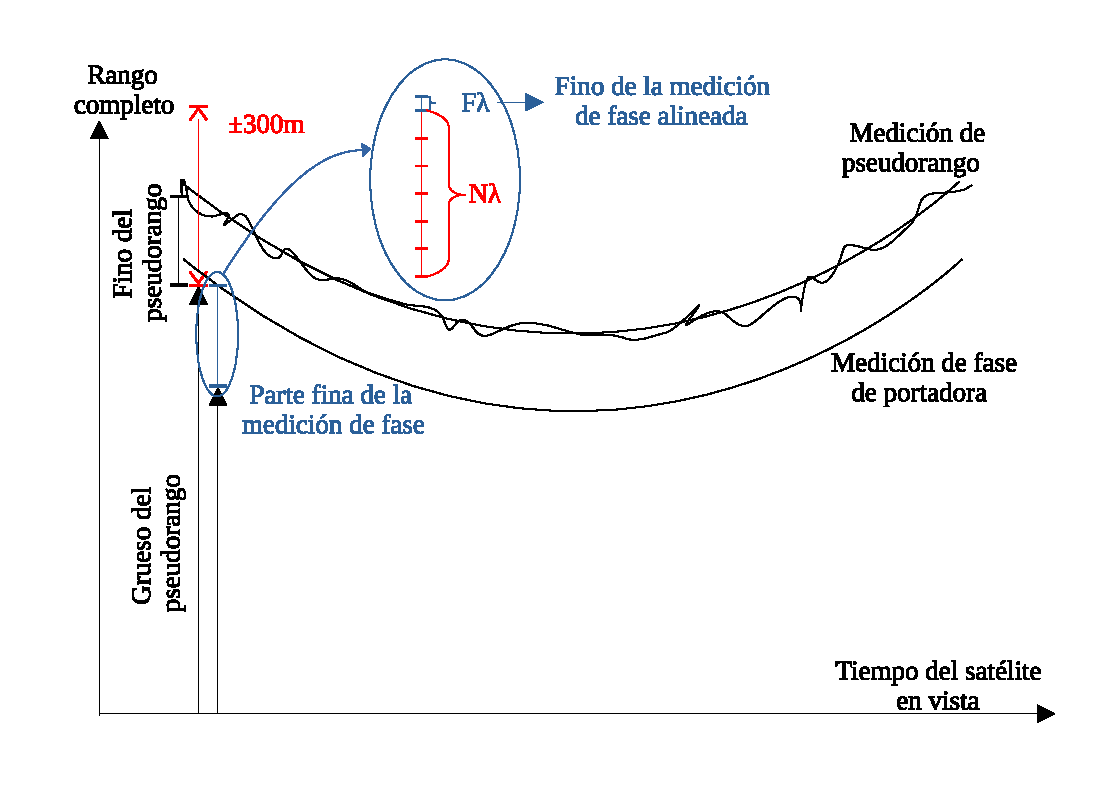
\includegraphics[width=1\textwidth]{/DGNSS/Parte_gruesa_fina.eps}
    \caption{Rango al satélite durante todo el tiempo que permanece en vista.}
    \label{fig:rrng_frng}
\end{figure}
	
	El chip tiene un periodo de $1/(1.023\,MHz) = 977.5\,ns \approx 1\,\mu s$, y el rango grueso expresado en segundos tiene una resolución de $2^{-10}\,ms = 976.5\,ns \approx 1\, \mu s$. De esta manera vemos que la parte gruesa del rango (medición de pseudorango) se redondea a la distancia que viaja la señal en un tiempo de \textit{chip}, es decir, tiene una resolución de aproximadamente 300\,m en distancia. Esto se puede observar en color rojo en la Fig.~\ref{fig:rrng_frng}. Ahora la parte que corresponde a cada señal, es decir, hay un valor por cada señal de la que se cuente con mediciones, es denominado rango fino. El mismo puede valer como máximo aproximadamente 1100\,m en valor absoluto debido al rango del campo que contiene esta información. Pero como es una medida de lo que le falta al rango grueso para llegar al rango verdadero, si este campo supera el umbral de los 300\,m ya mencionado, se le atribuye al rango grueso de manera que la parte fina vuelve a ser menor que 300\,m.
	
	La parte fina de fase de portadora se genera como un rango haciendo uso de mediciones de fase, al cual se le resta la parte gruesa del rango ya mencionada. Y a partir de aquí, se descarta el numero entero de longitudes de onda que contiene la parte fina (color rojo en Fig.~\ref{fig:rrng_frng}), resultando en una parte fina que esta solo formada por una fracción de longitud de onda (color azul). La cantidad de longitudes de onda enteras descartadas se guarda para poder descartar la misma cantidad en la próxima época con mediciones, de manera que la parte fina de la fase de portadora comience a acumular a partir de aquí. Esto es equivalente a alinear la integración del corrimiento doppler de la portadora (medición de fase) con el pseudorango al inicio de la acumulación. Esto se mantiene así hasta que no haya un salto de ciclo en los lazos de seguimiento de la portadora o que el rango fino de fase exceda su rango máximo. En caso de suceder esto, se vuelve a alinear, es decir, se reinicia la cantidad de longitudes de onda enteras que se descarta en el rango fino formado como rango menos rango grueso. 
	
	Cabe destacar que como el rango grueso está simplemente redondeado y no truncado a longitudes de un chip, puede estar por encima o debajo del rango verdadero. Por lo que el campo de rango fino, de pseudorango y fase podría ser tanto positivo como negativo.
	
	En el rover, qué recibe esta información, la manera de recuperar el rango completo de pseudorango es como la suma del rango grueso y del fino. Para fase de portadora, si queremos tener una alineación entre el pseudorango y el inicio de la generación, se puede sumar la parte fina con la parte gruesa, obteniendo un valor de ambigüedades dado. Pero si quisiéramos formar el rango completo con medición de fase directamente considerando que es igual a la parte fina, también es equivalente. Simplemente cambiaría el valor de las ambigüedades, que de hecho serían mucho mayores que en el caso de realizar la alineación. Esto no es un inconveniente ya que una vez resueltas estas ambigüedades solo queda fijar cuál es su valor y el rango obtenido con la medición tiene la precisión de las mediciones de fase.

\subsection{Campos de los mensajes MSM}\label{sec:campos_MSM}
	Todos los mensajes del tipo MSM tienen el mismo encabezado, que se puede observar en la Tab.~\ref{tab:MSMheader}. El mismo esta formado por los campos siguientes.
% Please add the following required packages to your document preamble:
% \usepackage[table,xcdraw]{xcolor}
% If you use beamer only pass "xcolor=table" option, i.e. \documentclass[xcolor=table]{beamer}
\begin{table}[]
\centering
\begin{tabular}{|l|c|}
\hline
\rowcolor[HTML]{C0C0C0} 
\multicolumn{1}{|c|}{\cellcolor[HTML]{C0C0C0}CAMPO} & \begin{tabular}[c]{@{}c@{}}Identificador\\ de campo\end{tabular}      \\ \hline
Número de mensaje                                   & DF002                                                                 \\ \hline
Identificador de la estación de referencia          & DF003                                                                 \\ \hline
Tiempo de la época GNSS                             & \begin{tabular}[c]{@{}c@{}}Específico de \\ cada sistema\end{tabular} \\ \hline
Indicador de múltiples mensajes MSM                 & DF393                                                                 \\ \hline
Reservado                                           & DF409                                                                 \\ \hline
Reservado                                           & DF001                                                                 \\ \hline
Indicador de correcciones de reloj                  & DF411                                                                 \\ \hline
Indicador de reloj externo                          & DF412                                                                 \\ \hline
Indicador de suavizado sin divergencia              & DF417                                                                 \\ \hline
Intervalo de suavizado                              & DF418                                                                 \\ \hline
Máscara de satélites GNSS                           & DF394                                                                 \\ \hline
Máscara de señales GNSS                             & DF395                                                                 \\ \hline
Máscara de celdas GNSS                              & DF396                                                                 \\ \hline
\end{tabular}
    \caption{Encabezado de los mensajes MSM.}
    \label{tab:MSMheader}
\end{table}

%\begin{figure}
%    \centering
%    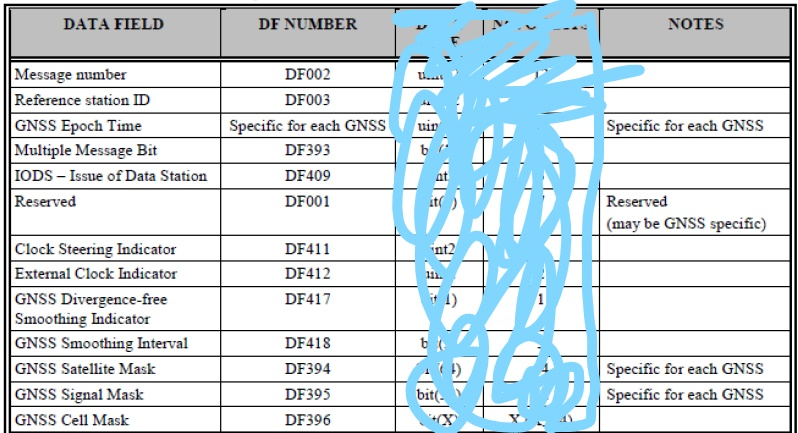
\includegraphics[width=0.8\textwidth]{/DGNSS/MSMheader.jpg}
%    \caption{Encabezado de los mensajes MSM.}
%    \label{fig:MSMheader}
%\end{figure}
\begin{description}[wide]
	\item[Número de mensaje] Especificador de que mensaje se está enviando.
	\item[Identificador de la estación de referencia] Número identificador que se le asignó a la estación de referencia. Para que el rover puedo identificar de qué base proviene el mensaje en caso de recibir mensajes de múltiples bases en simultaneo.
	\item[Tiempo de la época GNSS] Tiempo correspondiente a la época de toma de mediciones. Cada sistema GNSS lo empaqueta de distinta manera. En particular GPS especifica el tiempo como la cantidad de milisegundos transcurridos desde el inicio de la semana GPS (medianoche del sábado por la noche o domingo por la mañana).
	\item[Indicador de múltiples mensajes MSM] En alto si a continuación vendrán mensajes con mediciones para una misma época. En caso de que las mediciones fueron divididas en múltiples mensajes MSM, el rover deberá esperar a recibir el último mensaje para poder usar los datos que cada uno contiene.
	\item[Indicador de correcciones de reloj] Este campo indica si se están realizando correcciones de reloj al tiempo de receptor de la base que está generando los mensajes. Si se indica que se están haciendo las correcciones, las mismas deben asegurar que el reloj del receptor esté dentro de un rango de $\pm 1\,\mu s$ de error. En caso de indicar que no hay correcciones esta condición es menos restrictiva y el rango aumenta a $\pm 1\,ms$. También hay un estado que indica que no se conoce el estado de las correcciones, por lo que podrían estar haciéndose como no.
	\item[Indicador de reloj externo] Este campo indica qué tipo de reloj está usando el receptor, un reloj interno o uno externo. Y si fuera externo además se puede indicar si esta enganchado o no, en caso de no estarlo podría haber fallas en este reloj y que la información no sea confiable.
	\item[Indicador de suavizado sin divergencia] Este campo indica si se realiza un suavizado a las mediciones con un método sin divergencia (DFS por sus siglas en inglés), se realiza otro tipo de suavizado o ninguno.
	\item[Intervalo de suavizado] Es el periodo de integración en el cual se están promediando las mediciones de pseudorango con información de la fase de portadora. En caso de no hacer ningún tipo de suavizado esté campo se llena con ceros.
	\item[Máscara de satélites GNSS] Este campo va a ser de utilidad para el software decodificador para saber de qué satélites se están enviando mediciones. Es un campo de 64 bits donde cada bit corresponde a un satélite, en GPS corresponden a cada PRN comenzando por el primer bit que equivale a $\text{PRN}_1$. GPS tiene solo 32 satélites operativos por lo que se llenarán la primer mitad del campo con los satélites disponibles y la segunda mitad estará en cero siempre. En GLONASS ocurre lo mismo pero el primer bit corresponde al primer slot de frecuencia.
	\item[Máscara de señales GNSS] Este campo será utilizado por el software decodificador para saber qué señales tienen mediciones disponibles en los mensajes enviados. Tiene 32 bits y se corresponden con los identificadores de señal del estándar RINEX 3.01. Entonces, si en las mediciones hay disponibilidad de una señal para al menos un satélite, el bit correspondiente a esta señal se encuentra en alto.
	\item[Máscara de celdas GNSS] Este campo es de largo variable y condensa los últimos dos campos que se desarrollaron más arriba. Es una tabla de dos dimensiones que indica qué señal está disponible para cada satélite. Y es de largo variable ya que depende de la cantidad de señales y satélites disponibles, es decir, la cantidad de bits en alto en la máscara de señales y de satélites. El tamaño es $X = N_{sat}N_{sig}$, pero tiene una restricción a $X\leq 64$ por mensaje. En caso de superarse este número, hay que dividir los observables en distintos mensajes de manera que se cumpla con esta restricción. La primera fila de esta tabla corresponde a la señal con el identificador más chico (numéricamente), y así consecutivamente el resto de las filas. En las columnas sucede lo mismo pero con el identificador de satélites más chico.
\end{description}
	
	Habiendo descrito el encabezado del mensaje se puede proceder a describir cada campo del contenido del mismo, que en parte ya se introduce en la Tabla~\ref{tab:MSMall}. 
\begin{description}
	\item[Número entero de milisegundos en la parte gruesa del rango] A partir del rango grueso definido en la Sección~\ref{sec:rrng_frng}, se lo divide en una parte entera y fraccional (a milisegundos). La cantidad entera de milisegundos en el rango grueso está contenida en este campo.
	\item[Parte gruesa del rango módulo 1\,ms] En este campo va la parte fraccional en milisegundos que queda del rango grueso. En otras palabras sería el rango grueso menos el campo anterior.
	\item[Rangos finos de pseudorangos] La parte fina del rango en base a mediciones de pseudorango que se definió en la Sección~\ref{sec:rrng_frng}.
	\item[Rangos finos de fase de portadora] La parte fina que obtenemos de las mediciones de fase de portadora, tal como se describió en la Sección~\ref{sec:rrng_frng}.
	\item[Tiempo de enganche de fase de portadora] Es un indicador del tiempo en el cual el receptor lleva enganchado de manera continua a una señal particular. Si ocurrió un salto de ciclo en el instante de toma de mediciones anterior, se debe reiniciar este campo a cero.
	\item[Indicador de ambigüedades de medio ciclo] En caso de transmitir mediciones de fase de portadora con polaridad no resuelta es necesario setear este campo para que el software decodificador tenga esa información. Si el software decodificador no es capaz de trabajar con estas ambigüedades, va a descartar estas mediciones.
	\item[Relación portadora a densidad espectral de ruido] Esta medición es un estimado de la relación $C/N_0$ (portadora a densidad espectral de ruido) para cada señal del satélite. Si se completa con ceros significa que la medición no es válida.
\end{description}

	Hay campos tales como la desviación en frecuencia de la portadora que no son tratados con detalle ya que no se utilizan en este trabajo, pero tiene interés introducirlos para dar a entender la generalización que presentan los mensajes de múltiples señales. Lo mismo ocurre con el campo de información extendida de los satélites, que es un campo que todavía no está implementado y se reserva para uso futuro.\\


	Hasta aquí se desarrollaron los conceptos de posicionamiento relativo, o GNSS diferencial basado en fase de portadora. Este enfoque permite obtener soluciones de posición con una precisión en el órden de las decenas de centímetros o incluso centímetros. La ganancia es obtenida a costo de precisar trabajar no solo con un receptor GNSS, sino con varios, y no de manera aislada sino en conjunto. Para esto fue necesario presentar las distintas combinaciones que se pueden formar con las mediciones para desafectar errores y llegar a un escenario donde es factible resolver las ambigüedades que presentan las mediciones de fase. La complejidad que trae esto no es menor debido a que se precisa definir estándares de comunicación para los receptores operando en conjunto. Es por esto que se desarrollaron los puntos principales que sugiere el estándar RTCM para DGNSS, ahondando en los mensajes más importantes para conseguir el objetivo aquí planteado. Habiendo llegado hasta este punto resulta de interés poder validar lo desarrollado mediante ensayos con receptores GNSS operando en tiempo real. En el próximo capítulo se podrán observar resultados experimentales obtenidos en el laboratorio.
\chapter{Ensayos con receptores comerciales}\label{ch:ublox}
	Este capítulo comienza con el desarrollo experimental del trabajo y los ensayos que se basan en el marco teórico planteado en los Capítulos~\ref{ch:GNSS} y \ref{ch:DGNSS}. Primero se buscó replicar ensayos de posicionamiento RTK con receptores comerciales, que se sabe que logran obtener soluciones diferenciales con resolución de ambigüedades. Se plantearon ensayos con línea de base nula donde la comunicación entre los receptores operando en conjunto (base y rover) es cableada, en particular, por una interfaz UART. Se comenzó con un esquema cableado para poder dar pie a la implementación de este enlace en un receptor desarrollado en el lugar de trabajo que no cuenta con interfaz inalámbrica.
	
	Se exponen los materiales utilizados para las pruebas experimentales, principalmente haciendo hincapié en los receptores GNSS utilizados y su placa de evaluación. Por último, se muestran los resultados obtenidos en los ensayos.

% \section{Arquitectura del receptor}
\section{Placa de evaluación F9P u-blox}
	El módulo GNSS \textit{ZED-F9P} del fabricante \textit{u-blox} es un receptor comercial de alta precisión. Permite operación GNSS multisistema (GPS, GLONASS, Galileo, Beidou) y multibanda, además de operar con distintos sistemas de aumento de precisión como QZSS, SBAS o DGNSS. Al trabajar con el sistema GPS, el módulo puede operar con las señales L1C/A y L2C. Está especialmente pensado para aplicaciones donde los receptores operan en red, por lo que el mismo puede ser configurado como rover o estación de referencia en enfoques RTK~\cite{ZEDds}.

\begin{figure}
    \centering
    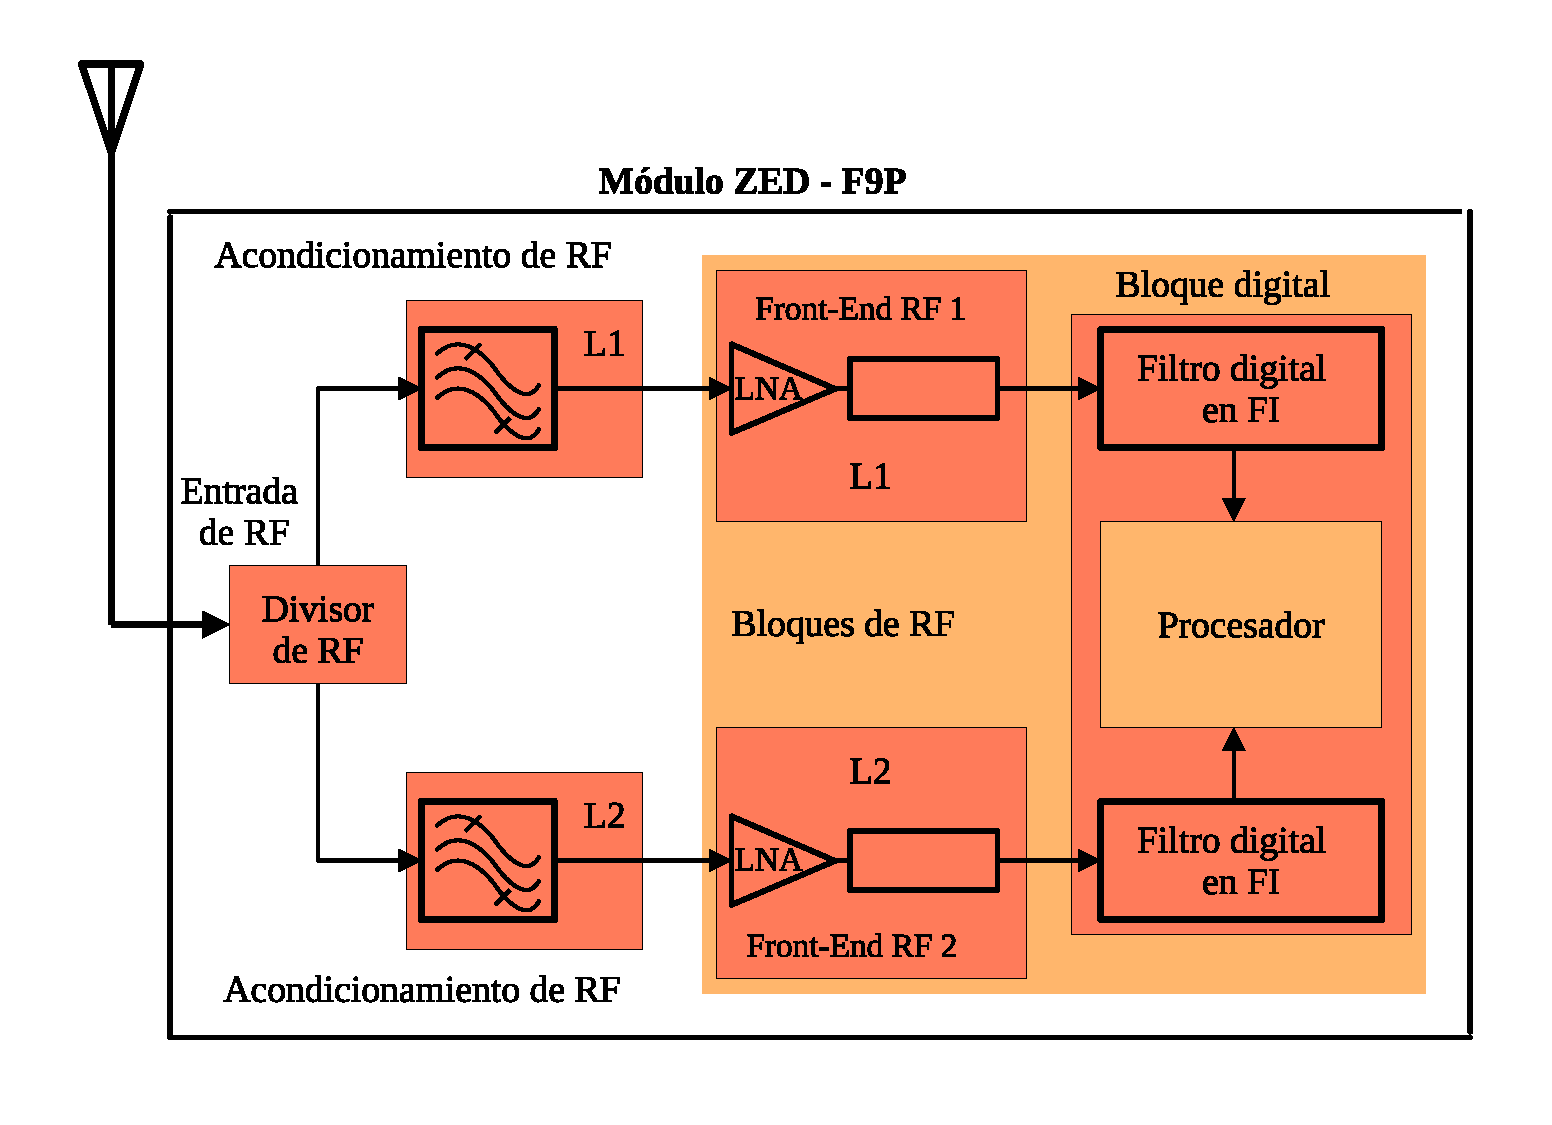
\includegraphics[width=0.85\textwidth]{/EnsayosUblox/BDublox.eps}
    \caption{Diagrama en bloques del módulo GNSS ZED-F9P.}
    \label{fig:BDublox}
\end{figure}
	Este módulo sigue a rasgos generales un esquema bastante universal de un receptor GNSS moderno como se puede observar en la Fig.~\ref{fig:BDublox}. Cuenta con una única antena GNSS, pero al trabajar a doble frecuencia inmediatamente debe dividir la señal para llevarla a la etapa del \textit{front-end} de RF para cada banda de frecuencias. Cada rama hace un filtrado pasabanda centrado en L1 y L2 respectivamente para quedarse con la señal de interés, y luego ingresa al bloque de RF correspondiente a cada señal. La etapa digital contiene los filtros en frecuencia intermedia y a partir de aquí toda la tarea de procesamiento de la señal es realizada por el sistema embebido. El mismo ejecuta todas las rutinas necesarias para la adquisición y luego seguimiento de las señales, obtención de la solución de posición y todas las validaciones necesarias para poder dar una solución confiable.
	
	Es interesante recordar cómo en los capítulos anteriores se analizó la cancelación de los retardos de hardware al combinar mediciones entre receptores, aquí queda en evidencia para un ejemplo de receptor real. Al contar con una etapa de RF individual para cada señal no hay razón para que los retardos instrumentales sean iguales en mediciones de distintas frecuencias. En caso de que los receptores sean diseñados correctamente para igualar estos retardos las consideraciones son distintas. Por eso es que a la hora del diseño se suele tener en cuenta este detalle incluso para aplicaciones de posicionamiento absoluto ya que es necesario que las señales lleguen sincronizadas a la etapa digital donde serán muestreadas. 
	
	En el lugar donde se desarrolla el presente trabajo se cuenta con un par de placas de evaluación para este módulo, con la finalidad de poder realizar experimentos RTK con un rover y una base. La placa de evaluación de la que se tiene disponibilidad es la \textit{C099-F9P}~\cite{C099_ds}, que además de contar con soporte para la interfaz con el módulo \textit{ZED} tiene un módulo de comunicaciones inalámbricas (\textit{ODIN-W2}). Este ultimo permite la conexión con otros receptores operando a distancia mediante comunicaciones de radio, en particular utilizando Wi-Fi o Bluetooth. En la Fig.~\ref{fig:EvBoard} se puede observar la placa de evaluación. Además de contar con la posibilidad de conectar una antena para la conexión inalámbrica, es posible utilizar los terminales cableados (conector J9 en la Fig.~\ref{fig:EvBoard}) para una comunicación serie entre la base y el rover mediante UART (Transmisor-Receptor Asíncrono Universal).
	
\begin{figure}
    \centering
    \includegraphics[width=0.8\textwidth]{/EnsayosUblox/ublox_foto.eps}
    \caption{Placa de evaluación \textit{C099-F9P}.}
    \label{fig:EvBoard}
\end{figure}
\subsection{Software de evaluación u-center}\label{sec:ucenter}
	El primer paso para poder hacer uso de los receptores aquí mencionados es poder configurarlos para que operen de la manera deseada. En la Fig.~\ref{fig:EvBoard} se puede ver el puerto serie (USB por sus siglas en inglés) con el que cuenta la placa de evaluación, a través del mismo se implementa la interfaz USB y UART del módulo ZED, y la interfaz UART del módulo ODIN. Para comunicarnos con el módulo ZED, el fabricante provee un software de evaluación GNSS llamado \textit{u-center}~\cite{u_center}. Este mismo permite generar y enviar los mensajes de configuración al módulo, ya sea para almacenar estos parámetros en memoria volátil como no volátil (RAM o FLASH). Si bien se utilizó el modulo ODIN para realizar pruebas preliminares al momento de familiarización con el software de evaluación y la placa, este fue deshabilitado en el momento en que se aprendió cómo realizar la comunicación cableada por UART.
	
	Además de poder configurar la placa de evaluación, mediante el mismo es posible visualizar los resultados en tiempo real mientras el receptor se encuentra operativo. Las distintas ventanas pueden mostrar la solución de posición obtenida, el nivel de precisión obtenido (en función de la varianza de las soluciones), el nivel de potencia de señal recibido para cada señal y satélite, los satélites en vista y los mensajes que está enviando el receptor. Esto último es de utilidad en aplicaciones diferenciales donde podemos observar qué mensajes está enviando la base. Se transmite también un indicador del tipo de solución obtenida, el mismo puede estar en los siguientes estados

\begin{itemize}
	\item 3D: Cuando el receptor está operando individualmente.
	\item 3D/DGNSS: Cuando el receptor está recibiendo mensajes RTCM.
	\item 3D/DGNSS/FLOAT: Cuando el receptor está estimando ambigüedades flotantes y no está logrando fijarlas.
	\item 3D/DGNSS/FIXED: Cuando el receptor logró resolver ambigüedades enteras y fijarlas.
\end{itemize}
	En la Fig.~\ref{fig:ucenter} se puede observar un ejemplo de lo que muestra \textit{u-center} para una configuración diferencial con el software conectado al rover habiendo resuelto ambigüedades.
\begin{figure}
    \centering
    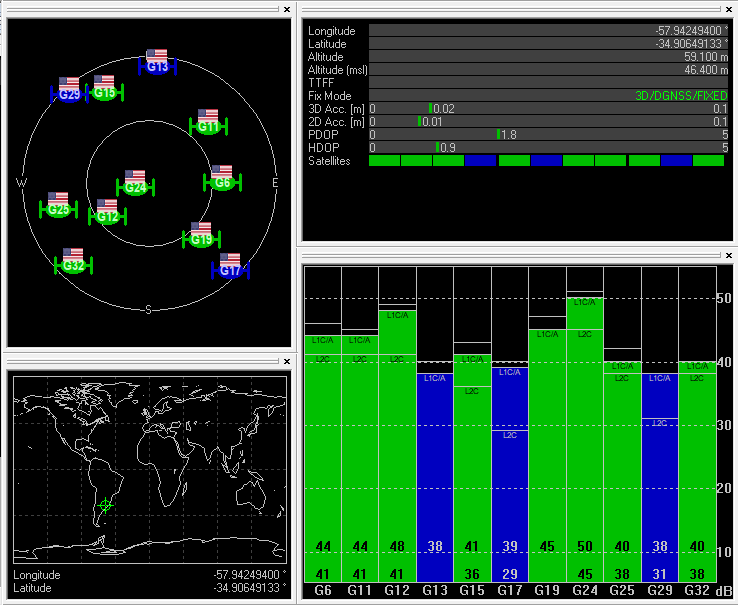
\includegraphics[width=0.7\textwidth]{/EnsayosUblox/UcenterViewFIX.png}
    \caption{Ventanas mostradas por \textit{u-center} al conectar el rover en un enfoque diferencial.}
    \label{fig:ucenter}
\end{figure}

\section{Esquema de ensayos con línea base nula}\label{sec:esquema_ZBL}
	En el Capítulo~\ref{ch:DGNSS} se detallaron los beneficios que traen los esquemas de combinación de mediciones con línea de base nula debido a la cancelación de errores y sesgos que presenta. Es por esto que se decide tratar con un escenario de este estilo para poder discutir aspectos respecto al desempeño obtenido. Además, al contar con una capa física en el enlace de comunicación que es cableada, no es posible realizar ensayos con grandes distancias entre los receptores, por lo que pensar en esta situación resulta lo más conveniente.
	
	La UIDET SENyT cuenta con una antena emplazada en la terraza del Departamento de Electrotecnia de la Facultad de Ingeniería, a la altura de un cuarto piso. La misma es una antena activa en las bandas L1 y L2 para los sistemas GPS y GLONASS. La señal que proviene de la antena es dividida mediante un diplexor como se observa en la Fig.~\ref{fig:EnsayoZBL}. El mismo cuenta con un desacople de continua para uno de los dos caminos en que se divide la señal, de manera que en caso de que se conecten dos receptores que den alimentación a la antena los mismos no sean cortocircuitados. Luego cada señal va a su respectivo receptor, rover y base. 

\begin{figure}
\centering
\subfloat[Diagrama del ensayo.]{%
  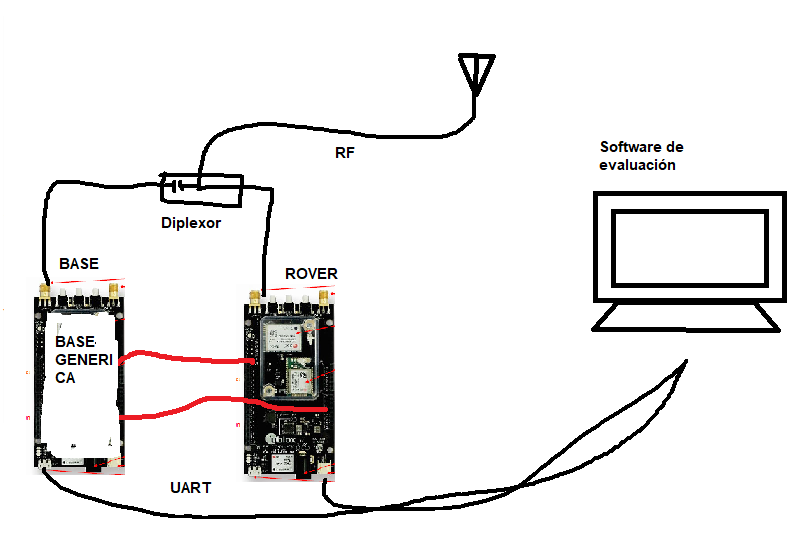
\includegraphics[width=0.6\textwidth]{/EnsayosUblox/EnsayoZBL.eps}
%  \caption{Esquema de ensayo con rover y base estacionarios, para linea base nula.}
  \label{fig:diagramaEnsayoZBL}
}
\centering
\subfloat[Diplexor con desacople de continua.]{%
  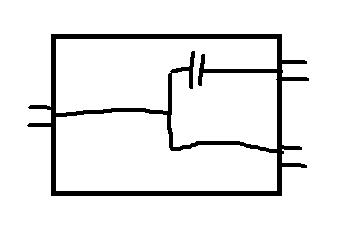
\includegraphics[width=0.4\textwidth]{/EnsayosUblox/diplexor.jpg}
  \label{fig:diplexor}
}
\caption{Esquema de ensayo con rover y base estacionarios, para línea base nula.}
\label{fig:EnsayoZBL}
\end{figure}

	La base debe ser configurada como tal, y al ser una estación de referencia estacionaria la misma debe enviar siempre la misma solución de posición. Para esto se puede configurar de dos modos, ingresar las coordenadas ECEF del ARP de la antena de la base para que el mensaje Tipo 1005 a transmitir contenga esta ubicación. La otra opción, en caso de no contar con las coordenadas, puede hacer que la base haga un relevamiento por determinado tiempo, filtre su solución de posición y la fije para usar esta solución en los mensajes RTCM a transmitir. Como la antena utilizada tiene sus coordenadas relevadas con suficiente precisión (por trabajos previos que se han desarrollado en el lugar), se puede utilizar el primer enfoque. Por último, es necesario indicar qué mensajes de observables transmitirá la base. En principio estos receptores pueden transmitir el mensaje Tipo 1005, los mensajes MSM 4 y MSM 7 para las constelaciones GPS (Tipos 1074 y 1077), GLONASS (Tipos 1084 y 1087), \textit{Galileo} (Tipos 1094 y 1097) y \textit{BeiDou} (Tipos 1124 y 1127). Se configuró para que envíe el mensaje Tipo 1005 y el MSM 4 de GPS (Tipo 1074), transmitiendolo por UART a una tasa de 460800 baudios.
	
	Como el módulo ODIN no está siendo utilizado ya que no hay ninguna comunicación inalámbrica en este ensayo, puede ser deshabilitado mediante un puente en los terminales de arranque seguro del ODIN-W2. En cuanto a la interfaz cableada, se conectó el terminal de salida de la UART ($T_X$) de la base al terminal de entrada UART ($R_X$) del rover y se les dió la misma referencia de tierra a ambas placas~\cite{moving_base_AppN}.
	
	En cuanto a la configuración del rover es necesario indicarle cuáles son los mensajes que recibirá por las distintas interfaces. En particular, hay que prestar atención a que espere recibir los mensajes que enviará la base por la interfaz UART y que tenga la misma velocidad de transmisión que la que se configuró para la base.

\section{Desempeño y calidad de la solución}
	El fabricante provee el protocolo UBX para loguear datos de los receptores. Es necesario establecer un cliente que pueda conectarse mediante un puerto serie al receptor y guardar los datos que fueron configurados para ser enviados. Haciendo las conversiones necesarias entre formatos se obtienen los datos de solución de posición para cada época y así poder analizar los resultados.
\begin{figure}
\begin{subfigure}{1\linewidth}
\centering
%\subfloat[Gráfico de dispersión de las soluciones de posición.]{%
  	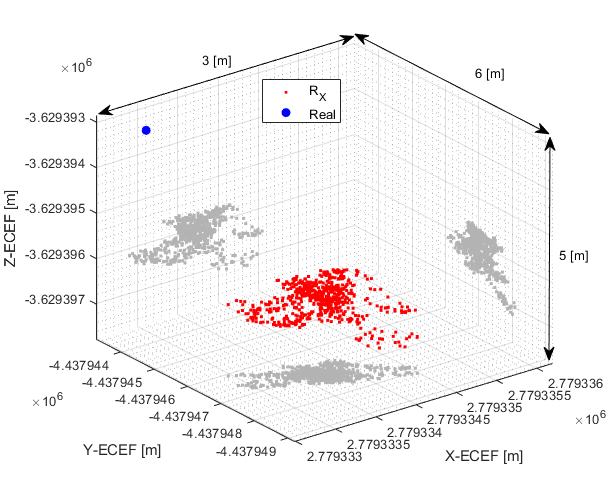
\includegraphics[width=0.7\textwidth]{/EnsayosUblox/ECEF_GNSS_ublox.png}
  	\caption{Gráfico de dispersión ECEF de las soluciones de posición con la posición real de la antena.}
    \label{fig:scatter_ublox_GNSS}
\end{subfigure}

\begin{subfigure}{1\linewidth}
\centering
%\subfloat[Errores para cada coordenada.]{%
 	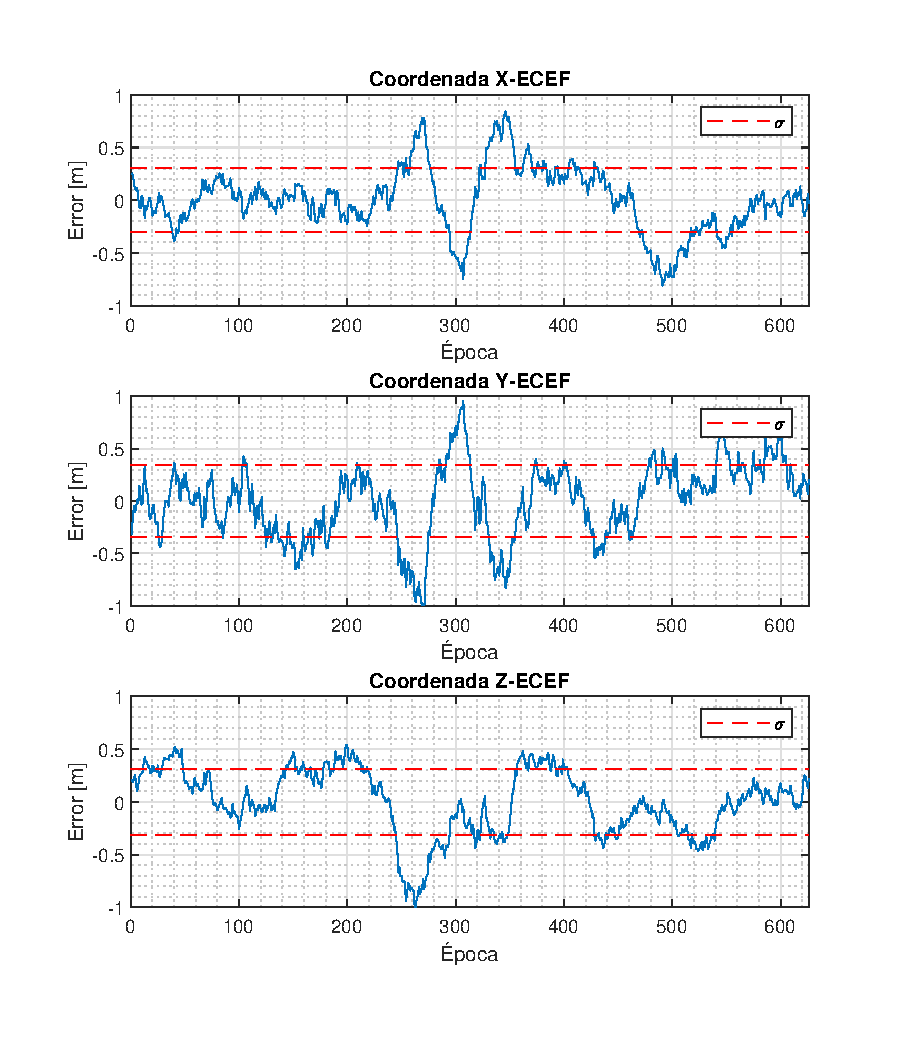
\includegraphics[width=0.7\textwidth]{/EnsayosUblox/ErroresXYZ_gnssUblox.eps}
 	\caption{Error de posición ECEF respecto a posición real.}
  	\label{fig:error_ublox_GNSS}
\end{subfigure}
\caption{Ensayo de un receptor comercial individual operando a doble frecuencia, sistema GPS, antena SENyT, con siete satélites en vista.}
\label{fig:ensayoGNSS_ublox}
\end{figure}
\subsection{Ensayo con rover operando individualmente}\label{sec:rover_alone}
	En primer lugar se puede ver un gráfico de dispersión de las soluciones obtenidas en coordenadas ECEF para un receptor \textit{u-blox} operando por su cuenta, sin pensar en un enfoque RTK. La Fig.~\ref{fig:ensayoGNSS_ublox} muestra este resultado con el receptor operando solo con el sistema GPS, a doble frecuencia (L1 y L2) y utilizando la antena activa ya mencionada anteriormente, que a partir de aquí será referenciada como `antena SENyT'. Se tomaron mediciones por diez minutos aproximadamente, a una tasa de 1\,Hz.
%\begin{figure}
%    \centering
%    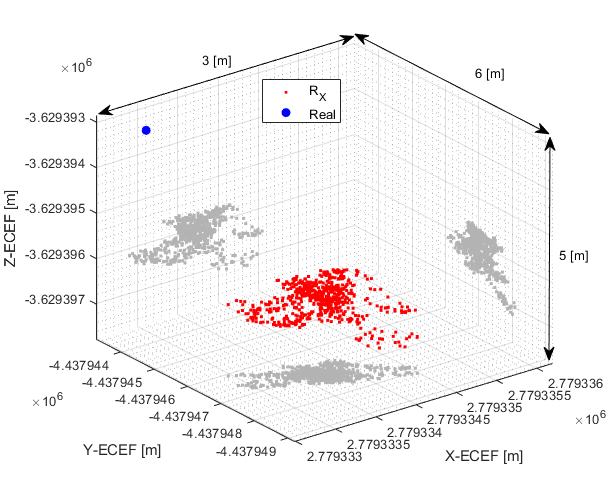
\includegraphics[width=0.7\textwidth]{/EnsayosUblox/ECEF_GNSS_ublox.png}
%    \caption{Gráfico de dispersión de las soluciones de posición para un receptor u-blox operando de manera individual. Ensayo a doble frecuencia, sistema GPS, antena SENyT, siete satélites en vista.}
%    \label{fig:scatter_ublox_GNSS}
%\end{figure}
%\begin{figure}
%    \centering
%    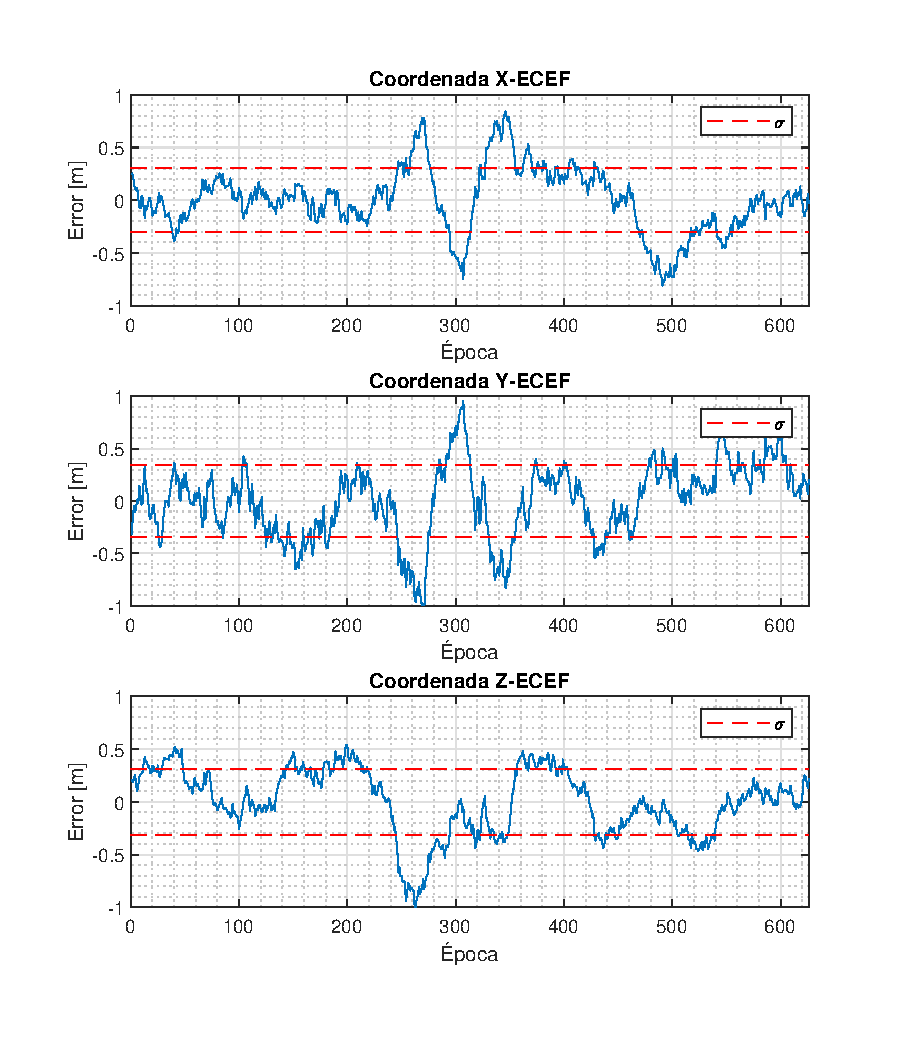
\includegraphics[width=1\textwidth]{/EnsayosUblox/ErroresXYZ_gnssUblox.eps}
%    \caption{Errores para cada coordenada. Ensayo a doble frecuencia, sistema GPS, antena SENyT, siete satélites en vista.}
%    \label{fig:error_ublox_GNSS}
%\end{figure}


	El gráfico de la Fig.~\ref{fig:scatter_ublox_GNSS} muestra la dispersión que presentan las soluciones obtenidas, se puede notar por la escala de los ejes que hay dispersión al nivel de los metros. Esto resulta esperable por lo que se ha planteado en el Capítulo~\ref{ch:GNSS} al trabajar con un enfoque GNSS no diferencial. Además, se indica la posición real de la antena SENyT utilizada en el ensayo para dejar en evidencia que al trabajar con un enfoque de posicionamiento absoluto además de tener la precisión mencionada, hay errores sistemáticos en la medición que no van a ser cancelados. Aquí el receptor está operando a doble frecuencia por lo que puede cancelar el efecto de la ionósfera, pero aún queda el efecto de la tropósfera. En cuanto a la nube de soluciones obtenidas por el receptor, las mismas alcanzan dispersiones del órden del metro (en las proyecciones es evidente cómo resulta esta dispersión para cada coordenada). Se observa que no hay una dispersión uniforme que se podría asociar a ruido, en cambio, las soluciones se concentran por zonas. Esto indica correlación temporal debido a errores que están presentes en la medición, tales como multicamino y demás errores en el pseudorango que se discutieron en el Capítulo~\ref{ch:GNSS}. El multicamino es un ejemplo muy evidente ya que depende de la geometría entre los satélites y el receptor, que va a cambiar con el tiempo.
	
	 Se puede agregar un gráfico de la desviación de cada coordenada respecto a la posición real de la antena (ver Fig.~\ref{fig:error_ublox_GNSS}). Se indica el valor medio que presentan estas desviaciones y el mismo es realmente notables en las tres coordenadas. Aquí se observa con mas detalle cómo las mediciones oscilan respecto a su valor medio pudiendo llegar a un metro de diferencia una de otra, confirmando lo que se discutió con la Fig.~\ref{fig:scatter_ublox_GNSS}. Pero al analizar la varianza de las soluciones obtenidas en base a la desviación estándar indicada en la figura, se ve que es similar para las tres coordenadas, obteniendo un valor de $3\sigma$ cercano al metro. 

\subsection{Ensayo RTK}\label{sec:RTK_ublox}
	Aquí es donde podremos observar la ganancia presentada por un esquema DGNSS, que logra entrar en modo RTK, comparando con los resultados obtenidos en el ensayo presentado anteriormente. Se trabajó con la base y el rover en un esquema como el presentado en la Sección~\ref{sec:esquema_ZBL}, los receptores operando a doble frecuencia, con el sistema GPS y utilizando la antena SENyT. Se tomaron muestras por trece minutos aproximadamente a una tasa de 1\,Hz.
	
\begin{figure}
\begin{subfigure}{1\linewidth}
\centering
%\subfloat[Gráfico de dispersión de las soluciones de posición relativa (linea de base).]{%
  	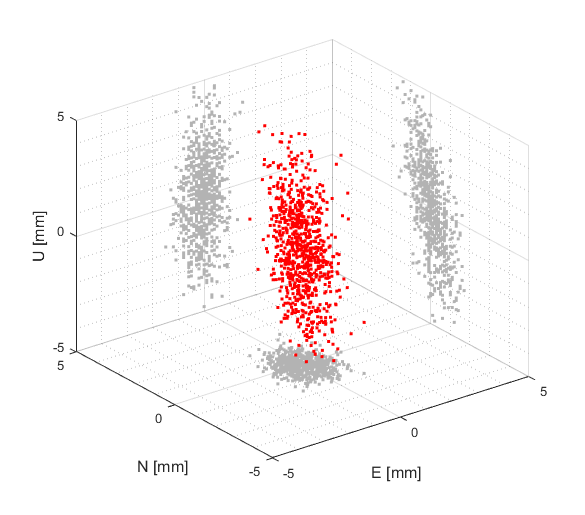
\includegraphics[width=0.7\textwidth]{/EnsayosUblox/ENU_DGNSSublox_scatter.png}
  	\caption{Gráfico de dispersión ENU de las soluciones de posición relativa (línea de base).}
    \label{fig:scatter_ublox_DGNSS}
\end{subfigure}


\begin{subfigure}{1\linewidth}
\centering
%\subfloat[Errores para la linea base en cada coordenada.]{%
 	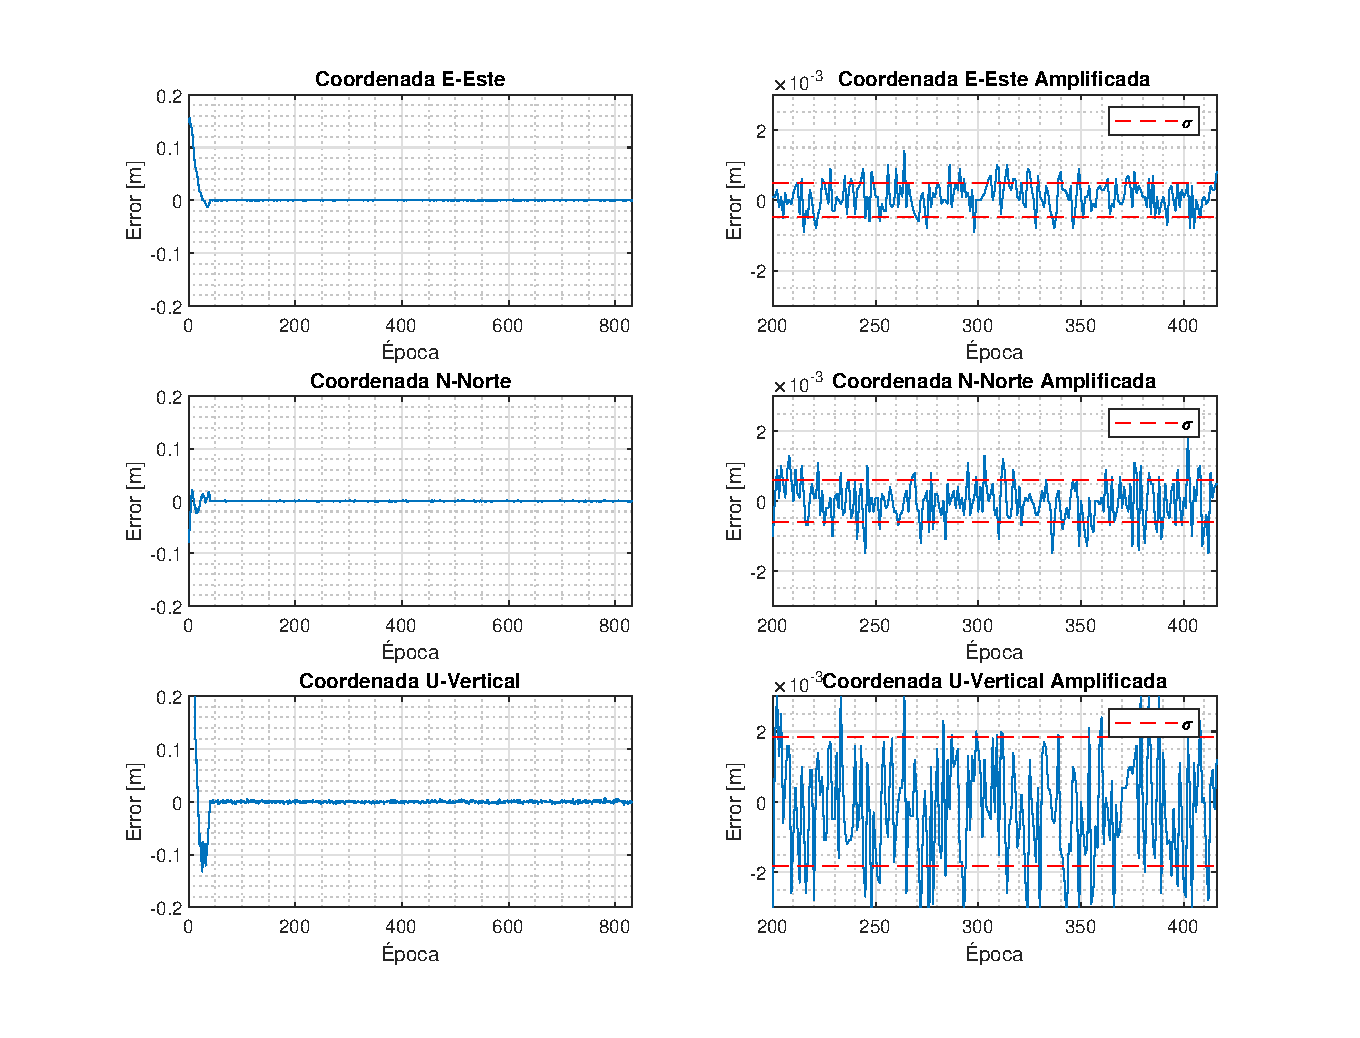
\includegraphics[width=0.7\textwidth]{/EnsayosUblox/ENU_timeplot_ublox_dgnss.eps}
 	\caption{Error ENU de línea base una vez fijadas las ambigüedades.}
  	\label{fig:error_ublox_DGNSS_fin}
\end{subfigure}
\caption{Ensayo RTK con línea base nula operando a doble frecuencia, sistema GPS, antena SENyT, con siete satélites en vista y receptor base comercial.}
\label{fig:ensayoDGNSS_ublox}
\end{figure}
	
	El diagrama de dispersión de la Fig.~\ref{fig:scatter_ublox_DGNSS} muestra cómo la nube de puntos se comprimió, teniendo muchos menos valores anómalos. En este caso se presentan los resultados en coordenadas ENU (por Este, Norte y Vertical) debido a que no se presenta una posición absoluta, sino la diferencia de coordenadas, es decir, la línea base. Pero como la base estacionaria tiene su posición fija conocida (en cualquier ensayo más allá de la línea de base nula), conocer la línea de base con precisión es también conocer la posición del rover con precisión. Se pudieron desafectar los errores sistemáticos obtenidos en el ensayo individual, efectivamente las soluciones están centradas en el origen ya que la línea de base es nula. Además, cabe destacar que si se presta atención a la escala de los ejes, se logró reducir en casi tres órdenes de magnitud la precisión lograda. 

\begin{figure}[h]
\centering
%\subfloat[Errores para la linea base en cada coordenada.]{%
 	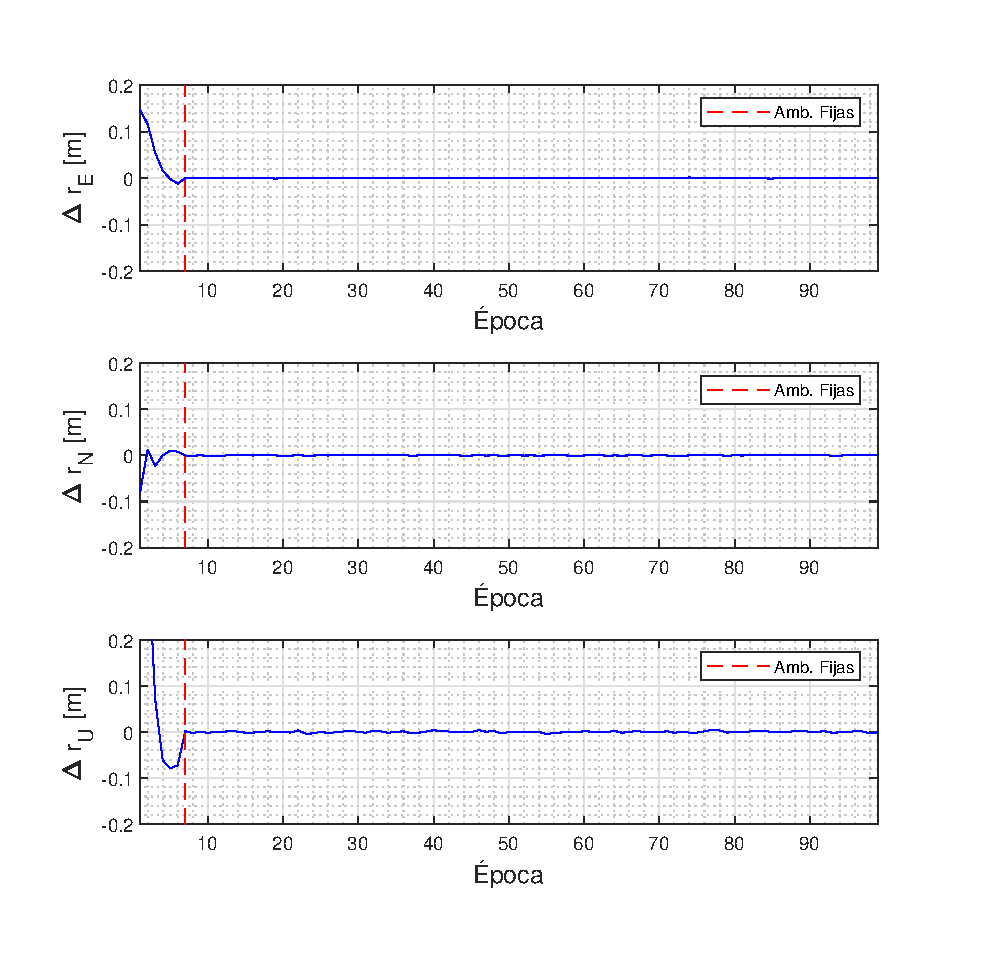
\includegraphics[width=0.7\textwidth]{/EnsayosUblox/ENU_DGNSSublox.eps}
 	\caption{Error ENU de línea base al inicio del ensayo. Ensayo RTK con línea base nula y base comercial.}
  	\label{fig:error_ublox_DGNSS_ini}
\end{figure}

	También se puede hacer un análisis respecto a la forma de la nube obtenida. Si observamos la proyección en el plano horizontal todas las mediciones se encuentran circunscritas dentro de una región circular de radio 2\,mm, que incluso siendo un poco menos restrictivos podríamos decir que la mayor parte esta dentro de la región de radio 1\,mm. Esto habla de una precisión en dos dimensiones, pero las proyecciones se pueden ver en otros planos. Si vemos las sombras en la coordenada vertical las mismas se extienden mucho más, teniendo que definir una circunferencia de hasta 5\,mm de radio para poder abarcar todas las mediciones. Esto es esperable para las soluciones de posición GNSS ya que por la distribución de los satélites de la constelación, se cuenta con poca diversidad de ángulos para los satélites en vista. Esto significa que hay una dilución de precisión (DOP por sus siglas en inglés) vertical más alta que en el resto de las dimensiones~\cite{kaplan}. Debido a este efecto, al considerar la precisión lograda en tres dimensiones los resultados no serán igual de favorables. Por esto es que si referimos a la Fig.~\ref{fig:ucenter} se puede ver la distinción que hace el software \textit{u-center} para presentar la precisión 2D y 3D, teniendo la 2D un valor más chico que la 3D. Tal cual como se explica cualitativamente en esta sección.

	Tal como se hizo para el ensayo con un único receptor, se puede analizar cómo resulta la evolución temporal de las coordenadas obtenidas para la solución diferencial. Hay que hacer una diferencia entre los distintos estados de la solución que ya se mencionaron en la Sección~\ref{sec:ucenter}. Al comienzo del ensayo los receptores todavía no han logrado entrar en modo RTK por lo que es esperable que la solución obtenida esté apartada en mayor medida del cero (valor que sabemos que tiene la línea base en este caso), tal como se puede observar en la Fig.~\ref{fig:error_ublox_DGNSS_ini}. Mientras el software intenta resolver las ambigüedades la solución converge de a poco al valor nulo en las tres coordenadas, primero logra estimar ambigüedades flotantes hasta conseguir fijarlas en números enteros. Aquí comienza a devolver una solución con el identificador 3D/DGNSS/FIXED, e instantáneamente se observa cómo la precisión (2D y 3D) aumentó considerablemente hasta llegar a valores como los que se observan en la evolución temporal de la Fig.~\ref{fig:error_ublox_DGNSS_fin} (notar el cambio en la escala del eje vertical). Incluso en ese instante se logró ver cómo la precisión 2D y 3D que indica el software de evaluación (\textit{u-center}) decrece considerablemente numéricamente.
	
\section{Conclusiones}
	Se presentaron los resultados para ensayos de receptores GNSS comerciales operando individualmente o en conjunto en un enfoque diferencial. Se corroboraron los valores numéricos planteados en el desarrollo conceptual y teórico de este trabajo, en particular para la precisión y cancelación de términos. Cabe destacar la limitación que existe en los enfoques de posicionamiento absoluto, ya que al tener las soluciones afectadas por errores sistemáticos debido a las condiciones de medición, no será posible cancelar estos errores ni realizando un filtrado de las soluciones. Teniendo en cuenta estos efectos en el modelo y cambiando el enfoque a uno de posicionamiento relativo, los resultados que obtienen estos receptores comerciales son realmente destacables. Sobre todo teniendo en cuenta la complejidad que presenta la implementación en un sistema embebido de un esquema de procesamiento diferencial. Además, se planteó una situación muy favorable en cuanto a la cancelación de errores y sesgos en la formación de dobles diferencias.
	
	Hasta aquí se pudieron plantear esquemas que ponen en evidencia de manera experimental lo que es bien conocido a nivel teórico. Se debieron diseñar las condiciones de ensayo para obtener los resultados presentados, lo cual implicó la familiarización con nuevos equipos y herramientas. Esto permite comenzar a desarrollar la parte del trabajo en donde hay implementación directa sobre un sistema embebido, en particular sobre un receptor GNSS desarrollado en la UIDET SENyT.

\chapter{Implementación del protocolo RTCM}\label{ch:Qseries}
	Este capítulo comienza con una descripción de la arquitectura y del funcionamiento de un receptor GNSS propietario de la UIDET SENyT, diseñado y fabricado por completo en el lugar de trabajo. Se desarrollan los aspectos relevantes a la hora de generar un estándar de comunicación RTCM, desde el lado de la estación de referencia. Por ultimo, se creó una pila de comunicación completa para el estándar ya mencionado, con su respectiva capa de enlace, capa de protocolo y capa de transporte. Además, aquí se discuten decisiones en la implementación de la capa física del enlace.
\section{Receptor Q Series propietario de SENyT}
	La línea de receptores Serie Q consiste en receptores GNSS con dos entradas independientes de antena, con posibilidad de operar en doble banda (L1 y L2) en ambas antenas. Pueden operar con los sistemas GPS y GLONASS, ademas de que los mismos estan diseñados con un factor de forma CubeSat estandarizado~\cite{Qseries_1}~\cite{Qseries_2} (ver Fig.~\ref{fig:Q}).
\begin{figure}
    \centering
    \includegraphics[width=0.6\textwidth]{/Qseries/receptorQ.png}
    \caption{Foto del receptor serie Q desarrollado por SENyT~\cite{Qseries_2}.}
    \label{fig:Q}
\end{figure}
\subsection{Arquitectura del receptor y funcionamiento}\label{sec:Qarq}
	Se puede referenciar nuevamente a la Fig.~\ref{fig:BDublox} para una idea a grandes rasgos del diagrama en bloques de un receptor GNSS. En este caso las diferencias principales consisten en la presencia de dos antenas, es por esto que se cuenta con dos cadenas de RF independientes, para cada antena. Esta etapa divide la señal por banda y luego diplexa cada banda a la etapa posterior que es separada para cada frecuencia. La etapa posterior, correspondiente al \textit{front-end} de RF es realizada por un circuito integrado (NT1065 de NTLab). La etapa digital esta implementada en una FPGA, que en particular, sintetiza un procesador de la arquitectura LEON3. La etapa previa de correlación también es implementada mediante descripción de hardware para lograr mayor eficiencia de procesamiento y cuenta con 24 canales independientes para señales en L1 (L1C/A) de GPS/GLONASS y 12 canales para la banda L2 (señal L2C) de GPS.

	El esquema de procesamiento se basa en un sistema operativo de tiempo real (RTOS por sus siglas en ingles). Se detalla la operación a simple antena y con el sistema GPS ya que es la modalidad en la que fue utilizado el receptor a lo largo de este trabajo. En términos generales, el funcionamiento del receptor en un arranque en frio consiste en que la etapa de seguimiento (\textit{tracking} del ingles) comience a buscar las señales de GPS que esta recibiendo. Si no tiene información de su posición y del tiempo absoluto al arranque no existe manera de que conozca cuales son los satélites de la constelación que estarán en vista. La opción mas directa con la que cuenta el receptor es comenzar a hacer una búsqueda de todas las señales que transmiten los satélites GPS, las diferenciaremos por su PRN. De esta manera, la etapa de seguimiento busca presencia de la señal haciendo la correlación con la PRN1 para todos los retardos posibles. Se puede estimar dentro de que retardos realizar la búsqueda ya que conocemos valores limites de los rangos que hay entre un receptor en la Tierra y la constelación de satélites. Pero ademas de realizar una búsqueda para todos los retardos, es necesario contemplar el efecto \textit{doppler} que afecta a la señal. Se pueden poner cotas de acuerdo a la dinámica conocida del receptor, por lo que se reduce el rango de frecuencias en las que debe realizar la búsqueda.
	
	El receptor termina realizando una búsqueda de la señal en un plano de retardo frecuencia, con limites impuestos por las condiciones de borde del problema de búsqueda. Esto comienza con el primer satélite hasta llegar al ultimo, esta parte de la búsqueda se conoce como búsqueda en ciego. En caso de encontrar 4 satélites en vista antes de llegar al ultimo, cambia el enfoque. Al momento de contar con 4 satélites, el receptor puede resolver su posición (con el grado de calidad impuesto por una solución no redundante). Una vez que el receptor pudo obtener su posición y haciendo uso del mensaje de navegación para obtener el almanaque o efemérides de los satélites puede tener conocimiento de los satélites que se encuentran en vista. De esta manera deja de ser necesario buscar uno por uno para cada PRN, sino que puede ir directamente a buscar a los que conoce que puede encontrar.
	
	Un enfoque distinto al de la búsqueda ciega podría ser uno en el que se le provee un almanaque al receptor con los satélites que debería tener en vista para esa época (y las épocas cercanas), desde el encendido del equipo. De manera de poder reducir la lista de búsqueda e ir a buscar directamente los satélites de los que si se están recibiendo señales.
	
	Esto comentado aquí es respecto a la etapa de seguimiento, una vez que la señal se encuentra en seguimiento pasa a la etapa de adquisición que lo que hace es obtener el mensaje de navegación modulado en la señal. Posterior a esto se pasa a las rutinas de navegación que son las encargadas de resolver la posición del receptor.
\subsection{Manejo de tiempos y sincronización en el receptor}\label{sec:times}
	A lo largo del presente trabajo se ha hecho hincapié en la importancia del manejo de tiempos en receptores GNSS. En particular, al trabajar con aplicaciones de precisión es indispensable prestar atención a esto ya que errores en la sincronización o etiquetado de tiempo tienen un impacto directo en las mediciones de fase de portadora o pseudorango. 
	
	Es necesario plantear una distinción entre los distintos sistemas de referencia temporal que existen en el receptor tratado en este capítulo. Teniendo en cuenta que el mismo está implementado sobre un sistema embebido, que a su vez se implementa en una FPGA, hay que basar la temporización en las escalas temporales que utiliza la FPGA para referencia. 
\begin{itemize}
	\item Sello de tiempo de la FPGA ($T_s$): Es un contador de tiempo en base a ciclos de la FPGA. 
	\item Tiempo del receptor ($t_r$): Cuenta de tiempo que lleva el propio receptor en base a $T_s$ de la FPGA. Podría estar inicializado distinto que $T_s$, pero necesariamente van a correr a la misma tasa ya que son generados del mismo lugar.
	\item Tiempo de recepción ($t_R$): Cuenta de tiempo que lleva el receptor en base al tiempo del sistema. Es el tiempo con el que se mide la recepción de las señales, por lo tanto tiene un sesgo y deriva distintos a los dos tiempos mencionados anteriormente.
\end{itemize}
\begin{figure}
    \centering
    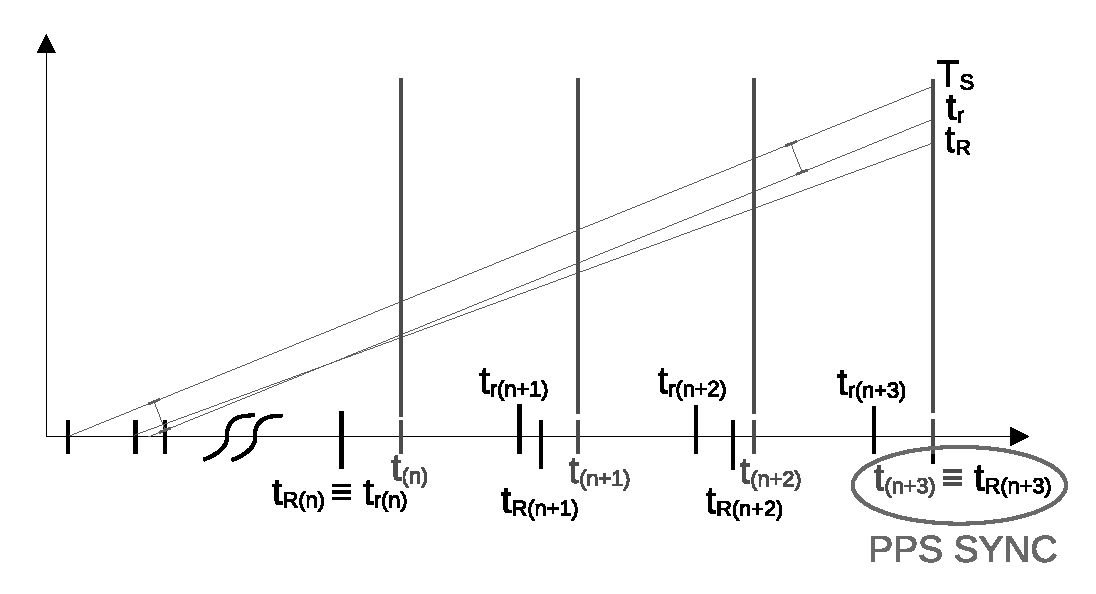
\includegraphics[width=0.9\textwidth]{/Qseries/tiempos_Q.eps}
    \caption{Evolución de cada referencia temporal en los receptores serie Q.}
    \label{fig:tiemposQ}
\end{figure}
	La inicialización que se hace del tiempo de receptor es a través del tiempo de transmisión que se obtiene del mensaje de navegación. Sin ningún tipo de información lo mejor que se puede hacer es estimar el tiempo de recepción como el tiempo de transmisión sumado al tiempo medio de viaje de la señal. Considerando los satélites GPS a una distancia media de 20000\,km, el tiempo de viaje resulta aproximadamente 70\,ms. Una vez inicializado, este tiempo corre a la misma tasa que el sello de tiempo de la FPGA. En cambio, el tiempo de recepción no es ajustado hasta que no haya solución de navegación y se resuelva la época para la cual se cuenta con mediciones. Como este tiempo está basado en el tiempo del sistema, va a tener su propia deriva pero es llevado a un valor de sesgo nulo (al menos para la resolución manejada en el receptor). El mismo es ajustado segundo a segundo hasta lograr una sincronización a los pulsos por segundo (PPS por sus siglas en inglés) del tiempo del sistema GPS, activando la bandera PPS SYNC que se puede observar en la Fig.~\ref{fig:tiemposQ}.
	
	El proceso de ajuste de tiempo de recepción hasta lograr la sincronización PSS, se realiza en conjunto entre la etapa de adquisición y la de navegación. Al momento de contar con solución, es posible medir el sesgo que existe entre el tiempo de recepción de la señal con los PPS. Esto es algo realizado por navegación, que al detectar este sesgo le indica a la etapa de adquisición que será necesario ajustar el tiempo de correlación para lograr el sincronismo. En caso que $t_R$ esté atrasado con respecto al PPS habrá que acortar el tiempo de integración y en caso contrario, alargarlo. Esto no se realiza instantáneamente, sino paulatinamente para poder hacer más suave el ajuste. Como las correlaciones se realizan con un tiempo de integración de 10\,ms, generalmente entran 100 de estas por cada segundo. En caso de tener un sesgo mayor a 10\,ms se puede agregar o quitar una correlación de este segundo, hasta conseguir que el sesgo sea menor a este periodo. Al llegar a este punto será necesario alargar o acortar el periodo de una única correlación de todas las que entran en un segundo, hasta que se consigue el sincronismo PPS. Este procedimiento indica que las correlaciones terminan siendo sincrónicas a la etapa de navegación y no a los bits de datos de la señal en seguimiento~\cite{correlation}.
\section{Generación de mediciones}\label{sec:mediciones}
	Si bien existen enfoques DGNSS donde se transmiten correcciones en los mensajes, en particular, correcciones por los errores que se introducen en las mediciones, los mensajes con los que se trabaja aquí son los que envían las mediciones crudas. La estación de referencia transmite sus mediciones de pseudorango y fase de portadora (Sección~\ref{sec:observables}) a los rovers, según el estándar RTCM. Debido a esto que se menciona, es posible trabajar con las mismas mediciones que genera la etapa de navegación del receptor, es decir reutilizarlas y así ahorrar tiempo de procesamiento en las rutinas nuevas que se implementan. De igual manera tiene valor discutir cómo son generadas las mismas ya que es de importancia analizar cómo se espera que sea la calidad de las mismas o el nivel de correcciones que se le aplican a las mismas.
	
	A esta altura el lector ya conoce que el pseudorango se genera a través del tiempo de viaje de la señal. Lo interesante entonces es analizar cómo se halla el tiempo de transmisión y el de recepción. En particular, el tiempo de transmisión se halla con los siguientes parámetros generados en la etapa de correlación
\begin{itemize}
	\item Medios bits (MB): La cantidad de medios bits (o integraciones de 10\,ms completas) que transcurrieron desde el origen. 
	\item Fracción de MB: La parte fraccionaria de las integraciones de 10\,ms transcurridas.
	\item Estado del código: Fase del código de la señal en seguimiento, expresado en \textit{chips}.
\end{itemize}
	Y estos parámetros se relacionan de la siguiente manera para obtener el tiempo de transmisión
\begin{align}
	&\text{Tiempo de transmisión} \ = \\ &\left(\text{MB}*10 \ + \ \text{Fracción de MB} \right)/1000 \ + \ \text{Estado del código}/(1.023\cdot 10^6) \ \nonumber.
\end{align}
	Cabe destacar que se habla de integraciones enteras de 10\,ms al igual que de medios bits ya que el periodo de un bit en el mensaje de navegación es de 20\,ms. Y al tener el estado del código medido en \textit{chips} solo basta con multiplicar por el periodo de un \textit{chip} para llevarlo a una escala temporal. Luego el tiempo de recepción es el mismo tiempo $t_R$ que se mencionó en la Sección~\ref{sec:times}.
	
	En cuanto a las mediciones de fase de portadora, tal como se había introducido en el Capítulo~\ref{ch:GNSS}, la etapa de correlación deberá integrar el \textit{doppler} para obtener una medición de \textit{doppler} acumulado que es equivalente a la medición de fase de portadora. La misma está expresada en ciclos de portadora, por lo que habrá que utilizar la longitud de onda de cada señal con la que se toman esas mediciones si se quisiera llevarlo a metros. Es conveniente utilizarlo en ciclos para evitar conversiones aunque el estándar especifica que la transmisión del mismo debe hacerse en unidades de metros (ver Sección~\ref{sec:RTCM}).
\section{Pila de comunicación asociada a la interfaz RTCM}
	El receptor donde se implementa esta etapa del trabajo ya cuenta con una pila de comunicación llamada \textit{Integración y Test} (I\&T) que es utilizada para la comunicación por USB con un cliente que puede obtener datos del receptor. Esta es utilizada tanto para depuración como para poder visualizar los resultados que esta obteniendo el receptor de sus soluciones y parámetros mas importantes. La idea es crear una pila de comunicación independiente de la de I\&T, especifica para el protocolo RTCM. La misma cuenta con una capa física cableada asociada al par de terminales UART del receptor (en el bus de datos que se observa en la Fig.~\ref{fig:Q}) y deberá tener su propia capa de dispositivo, protocolo y transporte. En particular, la interfaz UART utilizada se configura para operar a una tasa de 230400 baudios. 
	
	Las rutinas que generan y empaquetan los mensajes RTCM serán invocadas cada vez que suceda el evento de que hay datos de rango disponibles. Esto es indicado por la etapa de navegación con un periodo de un segundo, por lo que la tasa con la que se enviaran los mensajes RTCM sera de 1\,Hz. Se obtienen los datos de las rutinas de navegación y a partir de ahí se revisa que se haya conseguido sincronismo PPS. Si estamos sincronizados a PPS se procede a generar y enviar los mensajes RTCM. En caso contrario no tiene sentido pensar en enviar mediciones crudas de la estación de referencia a un rover, ya que el receptor de la estación no puede asegurar que tiene un sesgo de reloj con respecto al tiempo del sistema lo suficientemente chico. Esto se puede observar en la Fig.~\ref{fig:diagramaflujo_RTCM}, donde vale la aclaración de que las rutinas del estándar RTCM y el resto de las rutinas del receptor están al mismo nivel porque se ejecutan paralelamente.

\begin{figure}
    \centering
	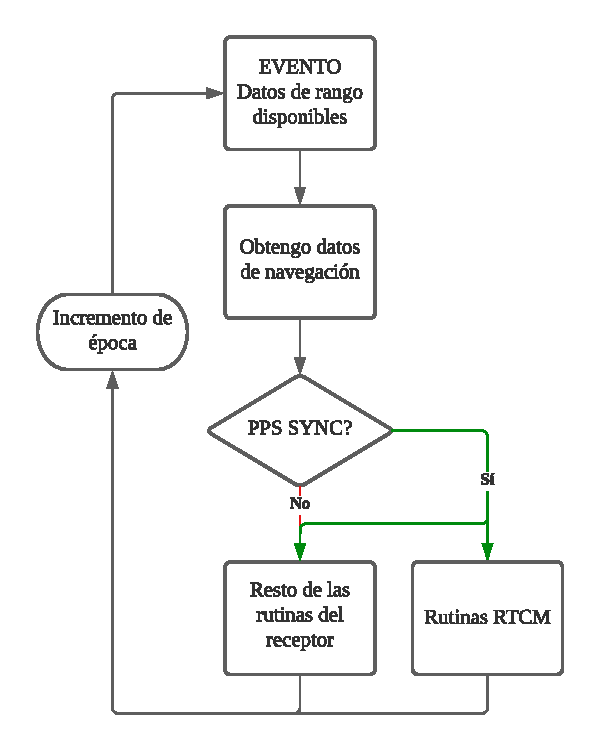
\includegraphics[height=0.6\textwidth]{/Qseries/Q_bd.pdf}
    \caption{Diagrama de flujo del llamado a la pila de comunicación RTCM.}
    \label{fig:diagramaflujo_RTCM}
\end{figure}

	En la Sección~\ref{sec:RTCM} se mencionaron las ventajas que presenta el enfoque más novedoso de mensajes de múltiples señales. Se decide implementar el mensaje Tipo 1005 que describe la estación de referencia y el Tipo 1074 (que corresponde al MSM4 de GPS). Ademas de lo ya mencionado respecto a los mensajes MSM, hay que tener en cuenta que los receptores comerciales \textit{u-blox} con los que se validará la recepción de los mensajes, no están preparados para trabajar con mensajes desactualizados, por lo que solo queda la opción de los MSM.
	
	Para conseguir eficiencia en términos de almacenamiento utilizado, el software del receptor realiza una distinción entre contenedores según tamaño. Siendo los contenedores los espacios de memoria donde se ubican los mensajes antes de ser enviados. Se reserva una cantidad fija de cada contenedor y la pila comienza a llenarlos con mensajes para enviar, cada vez que un mensaje es enviado se libera un contenedor y cuando llega el momento de enviar nuevos mensajes se pide un contenedor disponible para ser llenado. En caso de no contar con contenedores disponibles simplemente se omite el envío de mensajes RTCM hasta contar con contenedores libres.
	
	 Aquí se decide implementar tres contenedores, uno pequeño pensado para el mensaje Tipo 1005 (de largo fijo), uno de tamaño mediano pensado para los mensajes MSM (de largo variable pero acotados) hasta el MSM 4, y un ultimo contenedor grande que soporta todos los mensajes MSM (hasta el mas largo que es el MSM 7) e incluso otros mensajes del estándar que pueden ser mas largos que este tipo de mensajes. Los tamaños elegidos (en bytes) y la comparación con los mensajes que deberán contener se puede observar en la Fig.~\ref{fig:contenedores}, siempre quedando un remanente en cuanto a espacio entre el mensaje en su largo máximo y el limite del contenedor correspondiente.
\begin{figure}
    \centering
	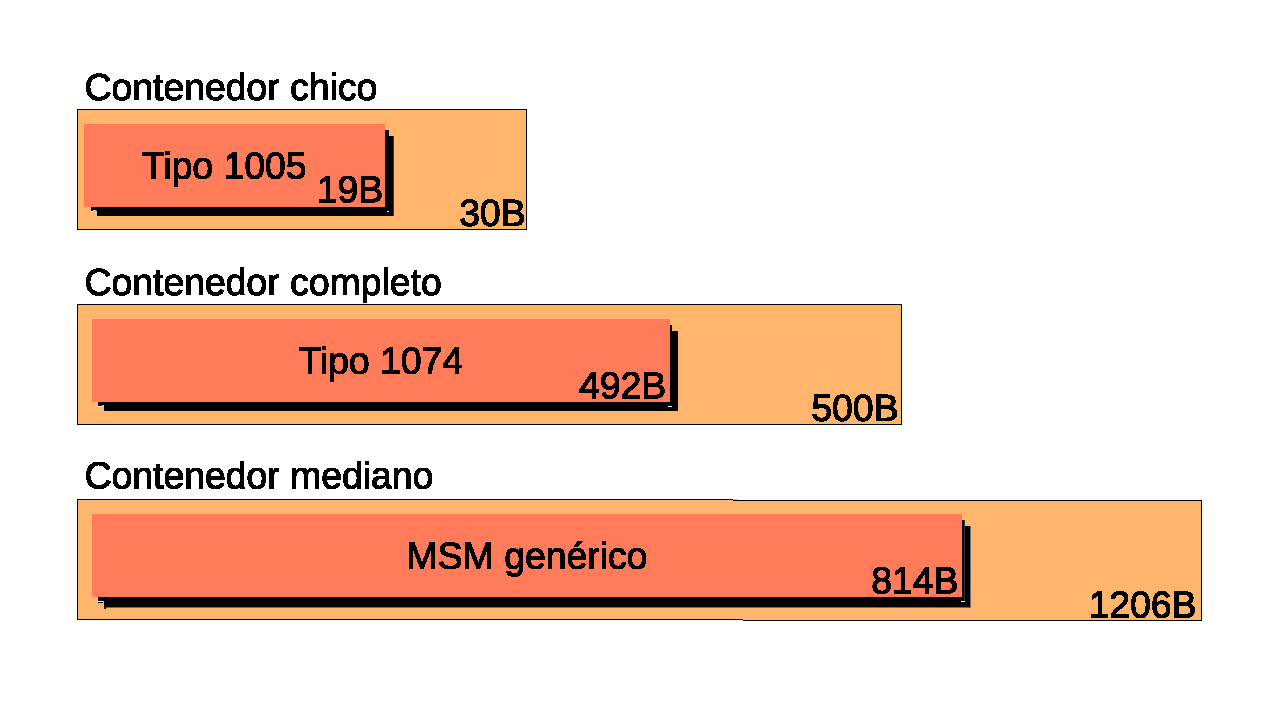
\includegraphics[width=0.9\textwidth]{/Qseries/Contenedores.eps}
    \caption{Tipos de contenedores de la pila de comunicación RTCM con los largos límites de cada mensaje (en bytes).}
    \label{fig:contenedores}
\end{figure}

	De esta manera, se utiliza siempre el contenedor chico para el mensaje Tipo 1005 y el contenedor mediano para el Tipo 1074. El contenedor grande no es utilizado pero tiene utilidad dejarlo en caso de que se implementen nuevos mensajes MSM en esta capa de protocolo RTCM. Esto ultimo permite la modularización para trabajos futuros que se realicen continuando este proyecto.
	
	Como solo se enviaran dos mensajes por segundo (uno de Tipo 1005 y uno de Tipo 1074), la única forma en la que se acumule más de un mensaje 1005 y un mensaje 1074 simultáneamente para ser enviados es si la pila de comunicación RTCM falla y no puede enviar alguno de los mensajes. Esto se puede verificar pensando en el largo máximo de ambos mensajes:
\begin{itemize}
	\item Tipo 1005: 9 bytes de mensaje + 6 bytes adicionales a la capa de transporte. 
	\item Tipo 1074: Depende del numero de satélites y de señales según
\begin{equation*}
	N_{bits} = \left[169 + N_{sat}\cdot(18+49\cdot N_{sig})\right] + 48 = 3929
\end{equation*}
	para $N_{sat} = 32$ y $N_{sig} = 2$. 
\end{itemize}
	En el caso más comprometedor hay que transmitir menos de 507 bytes entre los dos mensajes, sus respectivos encabezados y pies. Es decir que con una tasa de 9600 baudios alcanzaría para enviar ambos mensajes a una tasa de 1\,Hz. Con esto se argumenta que no sería necesario reservar mas de 1 contenedor de cada tipo, pero como se cuenta con memoria disponible se reservan 8 contenedores pequeños y 16 medianos.
	
	
\subsection{Capa de protocolo}
		
	Esta capa es la que se encarga de la generación de los campos correspondientes a cada mensaje. Ademas, realiza el pedido de contenedores para poder asignar espacio de memoria a los mensajes. 
	
	 En particular, para el mensaje Tipo 1005 se setean las coordenadas de la antena SENyT que se conocen con suficiente precision. Es similar a haber hecho un relevamiento de la ubicación en el momento, solo que aquí el relevamiento se hizo previamente. Las coordenadas ECEF que se transmiten son
\begin{description}
	\item[ECEF-X] 2779333.55
	\item[ECEF-Y] -4437943.40
	\item[ECEF-Z] -3629393.44
\end{description}

	Ademas, se le da un numero identificador a la estación base (ID = 2003) que sera respetado en todos los mensajes para que el rover pueda identificar a los mismos como provenientes de la misma base. Se setea el indicador de que se utiliza un oscilador interno y se indica que todas las mediciones crudas enviadas se toman en la misma época.
	
	Ahora para el mensaje Tipo 1074, se intenta aprovechar que existen implementaciones de acceso libre del estándar de comunicación RTCM bajo las bibliotecas de nombre RTKLIB. Las mismas consisten en un paquete de programas de posicionamiento GNSS de código abierto~\cite{rtklib}. La idea original fue reutilizar funciones de esta biblioteca que generan y empaquetan los campos de los mensajes, ya que están desarrolladas las funciones para los mensajes que son de interés aquí. Pero al intentar cargar el software del receptor con estas modificaciones se obtuvieron errores al reservar y acceder a memoria. La biblioteca esta implementada en lenguaje de programación C pero pensada para correr sobre una computadora, al querer replicar esto en un sistema embebido con prestaciones limitadas (sobretodo en cuanto a memoria) no se obtuvieron resultados satisfactorios. Debido a esto se procedió a implementar desde cero todas las funciones y rutinas que generan y empaquetan los campos del mensaje Tipo 1074.
	
	Ya se menciono que la etapa de navegación genera un evento cada segundo cuando hay set de observables disponible, la sección de la capa de protocolo que se encarga del manejo de los eventos busca este set de observables para reciclar lo que ya fue calculado para evitar procesamiento innecesario. Como esto sucede únicamente cuando el receptor puede asegurar sincronismo PPS, tiene sentido redondear la etiqueta temporal de las mediciones al segundo entero más cercano. Este es el tiempo de recepción que se utiliza en la generación del pseudorango. Se reutiliza la medición de fase de portadora que genera el receptor como se menciona en la Sección~\ref{sec:mediciones}. Y se reutiliza la estimación de relación portadora a densidad espectral de ruido ($C/N_0$) realizando un cambio de resolución para compatibilizar con el estándar.
	
	 Es necesario aclarar que se implementaron las rutinas para separar la parte gruesa de la fina como se detalló en la Sección~\ref{sec:rrng_frng}. Aquí es donde se mantiene una variable que lleva cuenta de la cantidad de números enteros de longitudes de onda que se le descontaron a la medición de fase de portadora, esto para cada señal de cada satélite. A los fines prácticos, cambiar el valor de las ambigüedades en la medición de fase es equivalente a tener un salto de ciclo ya que no se puede mantener fijo el numero de ambigüedades de una época a otra donde hubo salto de ciclo. Y cada vez que se cambia el valor de esta variable se reinicia el contador de tiempo en que la señal estuvo enganchada (ver Sección~\ref{sec:campos_MSM}), lo mismo sucede al haber saltos de ciclo ya que la variable ya mencionada debe ser reinicializada.
	
	Por otro lado, cada medición es etiquetada con el número de satélite del que proviene y con el identificador de señal según RINEX. A partir de esto se generan las máscaras de satélite, de señal y la de celdas. Quedó pendiente del Capítulo~\ref{ch:DGNSS} cómo resultan estos campos para un ejemplo de señales disponibles y satélites en vista. Si se cuenta con mediciones de los satélites GPS con PRN numero 12, 13, 15, 17 y 29. Se tienen mediciones de las señales L1C y L2L (según RINEX) de todos excepto del satélite con PRN 13, de este ultimo se cuenta solo con medición en la señal L1C. En la Tabla~\ref{tab:sat_mask} se ve que el bit correspondiente a cada PRN está en alto y para la máscara de señal (Tabla~\ref{tab:sig_mask}) se hace lo mismo para todas las señales disponibles. Según el estándar RINEX el identificador numérico que le corresponde a L1C es ID = 1 y a L2L es ID = 16. Con estos dos campos no hay manera de saber qué señal está disponible para cada satélite, para eso se arma la máscara de celda que se puede observar en la Tabla~\ref{tab:cell_mask}.
	
% Please add the following required packages to your document preamble:
% \usepackage[table,xcdraw]{xcolor}
% If you use beamer only pass "xcolor=table" option, i.e. \documentclass[xcolor=table]{beamer}
\begin{table}[]
\centering
\begin{tabular}{|l|l|l|l|}
\hline
\rowcolor[HTML]{9B9B9B} 
\multicolumn{1}{|c|}{\cellcolor[HTML]{9B9B9B}$PRN_{1\cdots 8}$}    & \multicolumn{1}{c|}{\cellcolor[HTML]{9B9B9B}$PRN_{9\cdots 16}$}    & \multicolumn{1}{c|}{\cellcolor[HTML]{9B9B9B}$PRN_{17\cdots 24}$} & \multicolumn{1}{c|}{\cellcolor[HTML]{9B9B9B}$PRN_{25\cdots 32}$} \\ \hline
00000000                                                 & 00011010                                                & 10000000                                                & 00001000                                                \\ \hline
\rowcolor[HTML]{9B9B9B} 
\multicolumn{1}{|c|}{\cellcolor[HTML]{9B9B9B}$PRN_{33\cdots 40}$} & \multicolumn{1}{c|}{\cellcolor[HTML]{9B9B9B}$PRN_{41\cdots 48}$} & \multicolumn{1}{c|}{\cellcolor[HTML]{9B9B9B}$PRN_{49\cdots 56}$} & \multicolumn{1}{c|}{\cellcolor[HTML]{9B9B9B}$PRN_{57\cdots 64}$} \\ \hline
00000000                                                 & 00000000                                                & 00000000                                                & 00000000                                                \\ \hline
\end{tabular}
\caption{Ejemplo de máscara de satélites para el sistema GPS. En vista PRNs: 12, 13, 15, 17 y 29.}
\label{tab:sat_mask}
\end{table}


% Please add the following required packages to your document preamble:
% \usepackage[table,xcdraw]{xcolor}
% If you use beamer only pass "xcolor=table" option, i.e. \documentclass[xcolor=table]{beamer}
\begin{table}[]
\centering
\begin{tabular}{|l|l|l|l|}
\hline
\rowcolor[HTML]{9B9B9B} 
\multicolumn{1}{|c|}{\cellcolor[HTML]{9B9B9B}ID$_{1\cdots 8}$}    & \multicolumn{1}{c|}{\cellcolor[HTML]{9B9B9B}ID$_{9\cdots 16}$}    & \multicolumn{1}{c|}{\cellcolor[HTML]{9B9B9B}ID$_{17\cdots 24}$} & \multicolumn{1}{c|}{\cellcolor[HTML]{9B9B9B}ID$_{25\cdots 32}$} \\ \hline
01000000                                                 & 00000001                                                & 00000000                                                & 00000000                                                \\ \hline
\end{tabular}
\caption{Ejemplo de máscara de señales para el sistema GPS. Disponibles: L1C y L2L.}
\label{tab:sig_mask}
\end{table}

% Please add the following required packages to your document preamble:
% \usepackage[table,xcdraw]{xcolor}
% If you use beamer only pass "xcolor=table" option, i.e. \documentclass[xcolor=table]{beamer}
\begin{table}[]
\centering
\begin{tabular}{|c|c|c|c|c|c|}
\hline
\rowcolor[HTML]{9B9B9B} 
\multicolumn{1}{|l|}{\cellcolor[HTML]{343434}\textbf{}} & \multicolumn{1}{l|}{\cellcolor[HTML]{9B9B9B}$PRN_{12}$} & \multicolumn{1}{l|}{\cellcolor[HTML]{9B9B9B}$PRN_{13}$} & \multicolumn{1}{l|}{\cellcolor[HTML]{9B9B9B}$PRN_{15}$} & \multicolumn{1}{l|}{\cellcolor[HTML]{9B9B9B}$PRN_{17}$} & \multicolumn{1}{l|}{\cellcolor[HTML]{9B9B9B}$PRN_{29}$} \\ \hline
\cellcolor[HTML]{9B9B9B}\textbf{L1C}                    & 1                                                       & 1                                                       & 1                                                       & 1                                                       & 1                                                       \\ \hline
\cellcolor[HTML]{9B9B9B}\textbf{L2L}                    & 1                                                       & 0                                                       & 1                                                       & 1                                                       & 1                                                       \\ \hline
\end{tabular}
\caption{Ejemplo de máscara de celda para el sistema GPS. $N_{sat}N_{sig} = 10$.}
\label{tab:cell_mask}
\end{table}

	En esta ultima etapa, al dimensionar el campo de la máscara de celda, se cuenta con la restricción del estándar de $N_{sat}N_{sig}\leq 64$. Pero además, hay una restricción de implementación que ya fue mencionada en la Sección~\ref{sec:Qarq}, el receptor cuenta con 24 canales de seguimiento por lo que nunca podrá contar con mayor cantidad de satélites. Ademas, solo puede recibir las señales L1C y L2L, por lo que el valor máximo que podrá tomar $N_{sat}N_{sig}$ es de 48. Lo que hace que el mensaje MSM 4 mas largo que puede enviar este receptor tenga 370 bytes de contenido. Los contenedores y campos para este mensaje se encuentran sobre dimensionados al caso general establecido por el estándar para dejar lugar a futuras modificaciones en la arquitectura del receptor.
	
	La capa de protocolo RTCM cuenta con una rutina para cada mensaje, una parte que genera los campos y otra que los empaqueta en el espacio de memoria que se reservo para el contenido del mensaje. 
\subsection{Capa de transporte}
	Habiendo mencionado los aspectos mas importantes que se implementaron en la capa de protocolo, que genera el contenido de los mensajes que puede enviar esta interfaz, se procede a tratar la capa de transporte creada. La misma se encarga de dar un formato compartido a todos los mensajes, independiente de su contenido, ademas de entregar los mismos a la capa de dispositivo para que los pueda encolar y direccionar para luego ser enviados por la interfaz UART de la capa física.
	
	Cuando se hizo referencia a los tipos de contenedores utilizados para cada mensaje, se detallo que quedaba espacio remanente incluso en los casos limites en los que los mensajes tienen mediciones de 32 satélites y a 2 señales. Es por esto que se puede agregar los 3 bytes correspondientes a encabezado y 3 bytes de paridad (ver Sección~\ref{sec:RTCM_format}) en el contenedor correspondiente a cada mensaje. El encabezado sigue los lineamientos ya descritos que plantea el estándar y lo mismo sucede para los 3 bytes de paridad.
	
	Se corroboró el correcto funcionamiento de esta capa enviando un mensaje con contenido conocido y genérico. Para la recepción y validación se utilizó un conversor de UART a ttyUSB disponible en el lugar de trabajo, y se recibió el paquete de bits por consola en una computadora. Como había correspondencia entre el encabezado y el contenido del mensaje que se enviaba, ademas de que los bits de paridad fueran los mismos que se obtenían al hacer el calculo por cuenta propia, se validó la capa de transporte creada para el estándar RTCM.
\section{Conclusiones}
	Se presentó toda la etapa de implementación y producción completamente propia de este trabajo. Se precisó pasar por una sección de familiarización con el receptor utilizado y con el proyecto donde se encuentra el software que corre sobre el sistema embebido. A partir de esto se planteó donde se deben realizar las modificaciones en el proyecto para añadir la interfaz completa correspondiente al estándar RTCM. Y luego se presentaron las decisiones tomadas a la hora de la implementación, junto con aspectos generales del proceso y resultados obtenidos. 
	
	Se obtuvo una pila de comunicación independiente de las demás presentes en el receptor serie Q, que permite una comunicación según el estándar RTCM entre una estación base y un receptor móvil GNSS operando en modo diferencial. Ademas, por la forma en la que se implementó permite la continuación del trabajo agregando el envío de nuevos mensajes sin necesidad de tener en cuenta capas inferiores en la comunicación, solo trabajando a nivel de protocolo. Es decir, generando los nuevos campos y realizando el empaquetado correcto de los mismos según cómo lo especifica el estándar.
	
	Es natural continuar a partir de aquí con una validación de la pila de comunicación creada, para poner en evidencia si la implementación es correcta y hasta dónde se pueden replicar los resultados obtenidos en el Capítulo~\ref{ch:ublox} con receptores comerciales.
\chapter{Validación en tiempo real}\label{ch:validacion}
	Este capítulo presenta la prueba funcional del enlace de comunicación implementado en el capítulo anterior. Se dejó en evidencia los resultados obtenidos al hacer uso de lo especificado por el estándar RTCM en un enfoque de posicionamiento GNSS relativo. En particular, replicando ensayos diferenciales que ya se discutieron en el Capítulo~\ref{ch:ublox}, pero ahora con un receptor base de desarrollo propio del lugar de trabajo. Además, se agregó un esquema de ensayo donde la línea de base no es nula. Se discute el desempeño obtenido en cuanto a uso de CPU en el receptor serie Q y en cuanto a la precisión de la solución de posición obtenida en el rover que recibe las correcciones.
\section{Receptor Serie Q utilizado como estación de referencia estacionaria}
	En esta etapa del trabajo se procede a poner en funcionamiento el receptor serie Q con el que se va a trabajar (introducido en el Capítulo~\ref{ch:Qseries}). En el capítulo anterior se puso a prueba la pila de comunicaciones creada, por lo que fue necesario cargar el software del receptor en el mismo, pero sin la necesidad de que reciba señales de los satélites GPS. Ahora es necesario llegar a este punto por lo que se debe conectar la antena en una de los conectores de antena del receptor (ver Fig.~\ref{fig:Q}) y corroborar que el mismo esté adquiriendo señales de los distintos satélites en vista. 
\begin{figure}
\begin{subfigure}{1\linewidth}
    \centering
	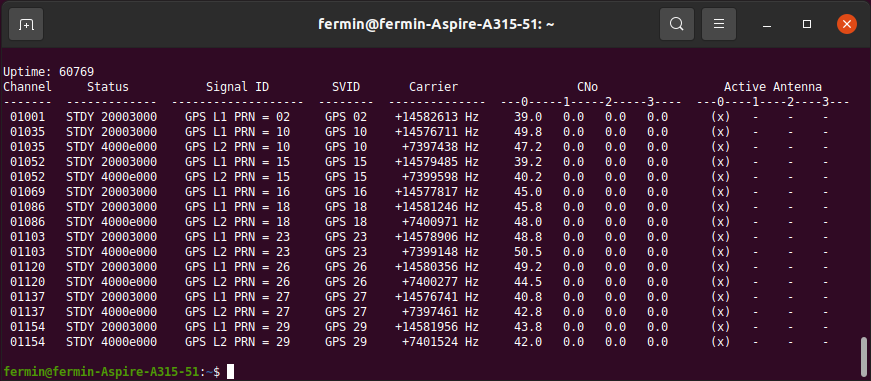
\includegraphics[width=1\textwidth]{/validacion/sgr_channelstatus.png}
    \caption{Estado de los canales.}
    \label{fig:sgr_channelstatus}
\end{subfigure}

\begin{subfigure}{1\linewidth}
    \centering
	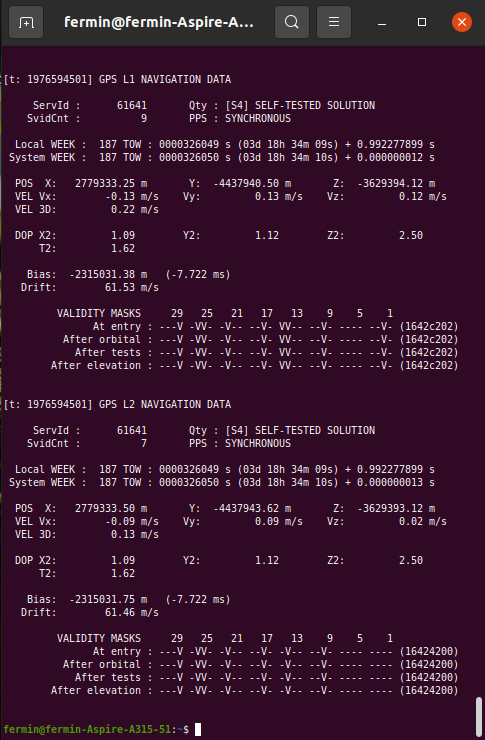
\includegraphics[height=0.9\textwidth]{/validacion/sgr_navigation.png}
    \caption{Datos de navegación.}
    \label{fig:sgr_navigation}
\end{subfigure}
\caption{Terminales cliente recibiendo datos del receptor operando en GPS $L_1/L_2$, 9 satélites en vista.}
\label{fig:sgrclient}
\end{figure}
	A través del comando de \textit{Linux} {\ttfamily `make'}, se puede compilar el ejecutable del software que se carga en memoria RAM del receptor. Una vez cargado este ejecutable en el receptor, desde una computadora y a través de uno de los puertos serie, se puede dar inicio al programa y conectar un cliente que escuche una de las interfaces de comunicaciones del receptor. 
	
	Se pueden visualizar los mensajes de consola que envía el receptor, los datos del estado de los canales y los datos de navegación. Los mensajes de consola dan información respecto a las rutinas que esta ejecutando el receptor, en general para depuración y a modo de conocer en qué estado se encuentra el mismo durante la ejecución. En el estado de los canales lo que se puede observar es el identificador de la señal que está en seguimiento por cada canal, en particular, el sistema, la frecuencia y a qué satélite corresponde. En la Fig.~\ref{fig:sgr_channelstatus} se puede observar que no todos los satélites GPS tienen señal en L2. Ademas, se puede ver la estimación de la frecuencia de portadora junto con el $C/N_0$ que se recibe. Es interesante notar como las frecuencias de portadora se mantienen siempre alrededor del valor conocido de L1 o L2, pero hay desviaciones debido al \textit{doppler} asociado a la dinámica de los satélites. 
	
	La visualización de los datos de navegación contiene la calidad de la solución, según las validaciones que haya pasado, las más significativas para los ensayos aquí tratados se muestran a continuación.
\begin{itemize}
	\item $S_0$: No hay solución.
	\item $S_2$: Hay solución pero no es segura ya que se utilizaron observables de solo cuatro satélites en vista.
	\item $S_4$: Hay solución y fue validada por el propio receptor ya que se cuenta con observables de más de cuatro satélites en vista.
\end{itemize}
	Además, se puede visualizar la solución de posición obtenida con cada una de las dos frecuencias (GPS L1 y L2) junto con la de velocidad en cada coordenada. Y por último, existe un indicador de si hay sincronismo PPS (ver Fig.~\ref{fig:sgr_navigation}), que en general es obtenido algunas épocas posteriores a haber conseguido una solución con calidad $S_4$. En particular, por las condiciones necesarias para que el protocolo de comunicación RTCM sea activado interesa la solución de mejor calidad.
	 
	En los ensayos aquí tratados se tuvo que tratar con el tiempo que demora el receptor en tener la primer solución de posición. Debido a la búsqueda ciega mencionada en el Capítulo~\ref{ch:Qseries}, según qué tan favorable sea la geometría de satélites al momento del ensayo, puede demorar mas tiempo o menos. La búsqueda de cada señal demora aproximadamente 18 segundos si se configura una búsqueda de la frecuencia de portadora con una incerteza de 14\,kHz. De esta manera, si los primeros cuatro satélites en vista corresponden a un SVID alto, es esperable que la primera solución sea obtenida luego de algunos minutos de búsqueda. Esto muestra el tiempo prolongado que lleva realizar cada ensayo con este receptor.

\section{Uso de CPU de las rutinas RTCM}
	Dentro de los mensajes que el receptor envía por consola, se puede observar un balance del uso de CPU de las distintas rutinas que ejecuta el mismo. En particular, tiene valor analizar el porcentaje de tiempo que es utilizado por las rutinas asociadas a la pila de comunicación RTCM. En general, el receptor operando con el sistema GPS y a doble banda, está cerca de la mitad del tiempo inactivo o esperando algún evento para ejecutar nuevas rutinas. Pero en caso de trabajar en una configuración demandante (en cuanto a tiempos de procesamiento) y esperar enviar mensajes RTCM, es de utilidad que la comunicación RTCM no se lleve gran parte del tiempo de computo utilizado por el receptor. 

	Esto se pudo poner a prueba y corroborar que la funcionalidad agregada no interfiere con el resto las tareas del receptor. En la Fig.~\ref{fig:CPU_usage} se puede observar el porcentaje de tiempo empleado por cada hilo. La primer columna indica el nombre para identificar cada hilo, la segunda muestra la cantidad de segundos que fueron utilizados por cada tarea en un lapso de 10 segundos y la última columna lo muestra en porcentaje. Los hilos correspondientes a la comunicación RTCM están resaltados y tienen por nombre PRTK y TRTK para la capa de protocolo y de transporte, respectivamente. Estos resultados corresponden con las condiciones presentadas en la Fig.~\ref{fig:sgrclient}, al estar con la bandera de sincronización PPS en alto se ejecutan todas las rutinas del protocolo RTCM y el mismo consume tiempo de CPU. Cabe destacar que la capa de protocolo es la que domina en cuanto a tiempo de computo, ya que es la que debe generar y empaquetar los campos, en cambio el uso asociado a la capa de transporte es realmente insignificante ya que solo agrega el encabezado, el pie y encola los mensajes a ser enviados. 
\begin{figure}
    \centering
	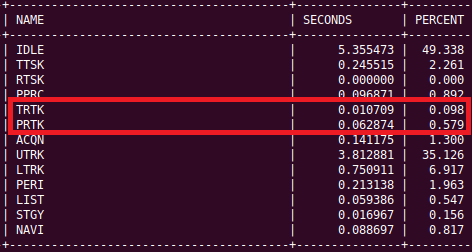
\includegraphics[width=0.6\linewidth]{/validacion/CPU_usage.png}
    \caption{Tiempo de uso de CPU del receptor por los distintos hilos.}
    \label{fig:CPU_usage}
\end{figure}
	De todas maneras, el tiempo total empleado por las rutinas RTCM no tiene peso frente a otras rutinas asociadas a la etapa de seguimiento como son UTRK y LTRK.
	
	En caso de no haber conseguido el sincronismo PPS, no se ejecuta ninguna rutina del protocolo RTCM por lo que el tiempo consumido por los hilos asociados al mismo es menor todavía. No es nulo ya que el manejador de eventos de la pila RTCM debe revisar si hay sincronismo para decidir si se ejecutan las rutinas o no.
\section{Ensayo DGNSS sin mediciones de fase}
	Durante una etapa del trabajo no era posible la utilización de las mediciones de fase debido a que las mismas no eran empaquetadas correctamente por la capa de protocolo RTCM. Se sacó provecho de esta situación para realizar ensayos de posicionamiento relativo utilizando solo mediciones de pseudorango. La base enviaba los mismos mensajes pero con mediciones de fase que no podrían ser utilizadas por el rover, de manera que el software decodificador las descartaría. El ensayo realizado es con una línea de base nula tal como se mostró en el Capítulo~\ref{ch:ublox}, con el receptor serie Q como base y el receptor del fabricante \textit{u-blox} como rover. El enlace de comunicación RTCM es cableado por la interfaz UART, el receptor está operando con el sistema GPS a doble frecuencia ($L_1/L_2$) y se tomaron mediciones por aproximadamente 15 minutos. Esto corresponde a 916 épocas cada 1 segundo (ver Fig.~\ref{fig:ensayoDGNSS_psrng_Q} para mayor detalle de las condiciones de ensayo).
	
	Se espera que el rover no pueda entrar en modo RTK y no logre estimar ni siquiera ambigüedades flotantes. Si las mediciones de fase de portadora no son correctas no existe forma de que las utilice para la estimación de las ambigüedades ya que ni siquiera va a haber consistencia entre las mismas mediciones de fase. Al realizar el ensayo se observa que el receptor logra entrar en modo \textit{3D/DGNSS}, es decir, está recibiendo mensajes RTCM y logra hacer un posicionamiento relativo, pero sin hacer uso de las mediciones de fase. 
\begin{figure}
\begin{subfigure}{1\linewidth}
\centering
%\subfloat[Gráfico de dispersión de las soluciones de posición.]{%
  	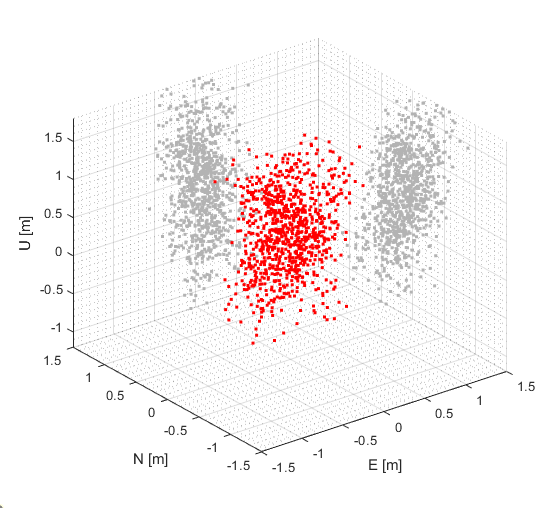
\includegraphics[width=0.7\textwidth]{/validacion/psrng_scatter_ENU.png}
  	\caption{Gráfico de dispersión ENU de las soluciones de posición relativa (línea base).}
    \label{fig:scatter_psrng_DGNSS_Q}
\end{subfigure}


\begin{subfigure}{1\linewidth}
\centering
%\subfloat[Errores para cada coordenada.]{%
 	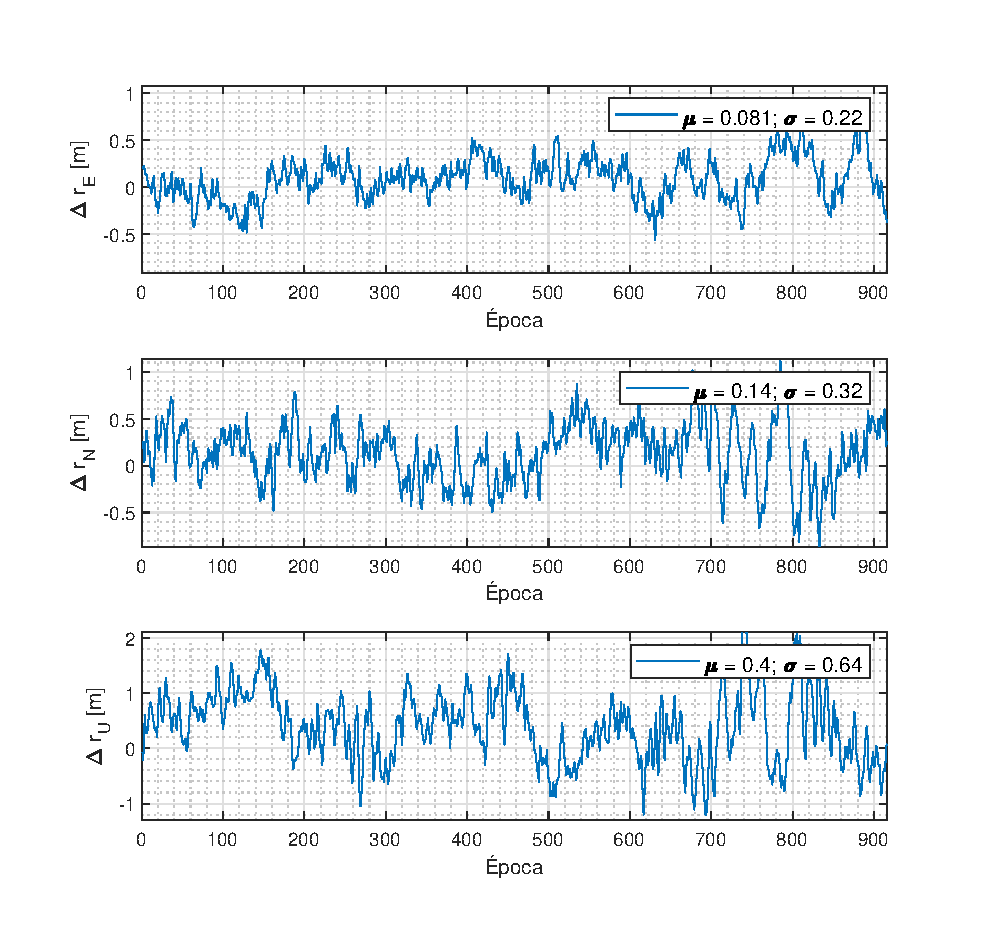
\includegraphics[width=0.7\textwidth]{/validacion/psrng_time_ENU.eps}
 	\caption{Error ENU de línea base.}
  	\label{fig:error_psrng_DGNSS_Q}
\end{subfigure}
\caption{Ensayo de posicionamiento relativo con línea de base nula operando a doble frecuencia, sistema GPS, antena SENyT, con ocho satélites en vista y receptor base Serie Q.}
\label{fig:ensayoDGNSS_psrng_Q}
\end{figure}

	Se presenta un diagrama de dispersión de la solución de posición relativa (ver Fig.~\ref{fig:scatter_psrng_DGNSS_Q}) y si bien no se logra bajar la dispersión de las soluciones obtenidas, u obtener mejor precisión, se observa cómo se pudo cancelar el efecto de los errores sistemáticos presentados en el ensayo del receptor operando individualmente (Sección~\ref{sec:rover_alone}). Esto es evidente al analizar las proyecciones de la nube de puntos en las distintas coordenadas, están todas centradas y además tienen una forma uniforme. A partir de esto se pone en evidencia cómo se lograron cancelar los errores en la medición debido a la formación de mediciones en dobles diferencias, resultando en una dispersión dominada por ruido de tipo gaussiano. Esta última es la principal diferencia que se presenta con los resultados obtenidos al trabajar con un receptor operando individualmente.
	
	Si bien al utilizar mediciones en DD, se obtienen diferencias en los resultados como se comparó aquí, la precisión lograda no tiene cambios significativos. Esto es debido a que se siguen utilizando mediciones de pseudorango para obtener la solución de posición, entonces la dispersión de las soluciones sigue estando dominada por el ruido en la formación del pseudorango. Los resultados se condicen con lo esperado debido al tipo de solución lograda por el rover, en el modo \textit{3D/DGNSS} no se consigue aprovechar la precisión de las mediciones de fase.
	
	Lo discutido con el gráfico de dispersión puede ser visto con mayor claridad en términos de los errores de línea base obtenidos con cada coordenada (Fig.~\ref{fig:error_psrng_DGNSS_Q}). Cada coordenada presenta un valor medio muy cercano al cero, y una varianza prácticamente igual al ensayo con el que se está comparando (receptor operando individualmente). La coordenada vertical presenta una media un poco desplazada del cero y una mayor varianza, pero esto se puede atribuir a los efectos que presenta la coordenada vertical debido a la geometría (mayor DOP discutido en el Capítulo~\ref{ch:ublox}).
\section{Ensayo RTK con línea de base nula y resolución de ambigüedades}\label{sec:RTK_fix_Q}\sectionmark{Ensayo RTK con línea de base nula}
\begin{figure}[t]
\centering
 	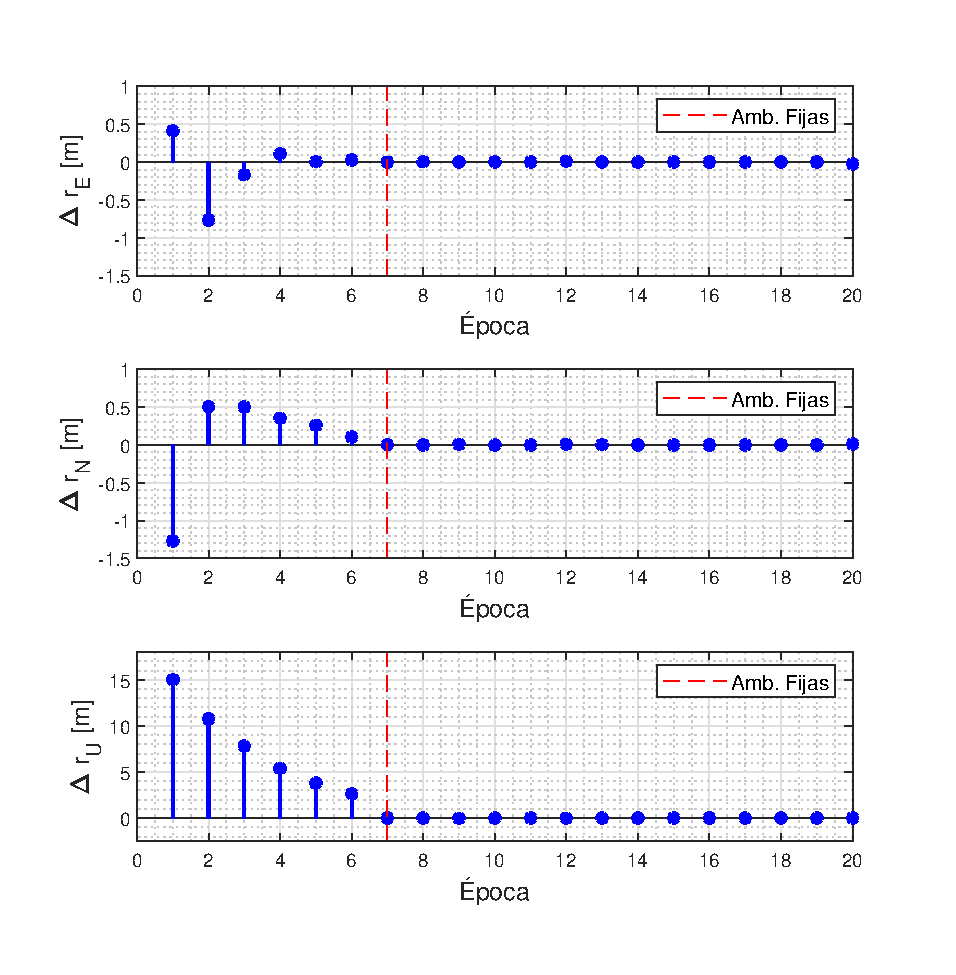
\includegraphics[width=0.7\textwidth]{/validacion/transition_float_fix_Q_DGNSS.eps}
 	\caption{Error ENU de línea base mientras intenta resolver ambigüedades. Ensayo RTK con línea de base nula y receptor base Serie Q.}
  	\label{fig:trans_float_fix_DGNSS_Q}
\end{figure}
	Una vez resuelto el inconveniente con el empaquetado de las mediciones de fase del receptor serie Q, se procede a ensayar un esquema de posicionamiento relativo RTK con receptores de distinto modelo. Con este ensayo se busca validar por completo el desarrollo e implementación realizados.
\begin{figure}
\begin{subfigure}{1\linewidth}
\centering
  	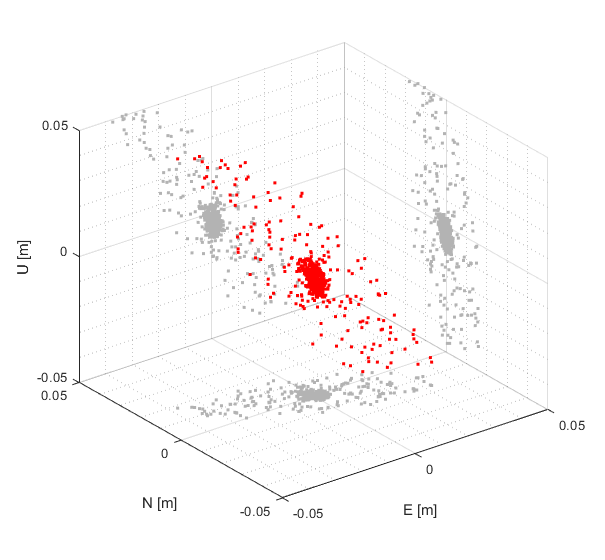
\includegraphics[width=0.7\textwidth]{/validacion/FIX_scatter_ENU.png}
  	\caption{Gráfico de dispersión ENU de las soluciones de posición relativa (línea base).}
    \label{fig:scatter_fix_DGNSS_Q}
\end{subfigure}

\begin{subfigure}{1\linewidth}
\centering
 	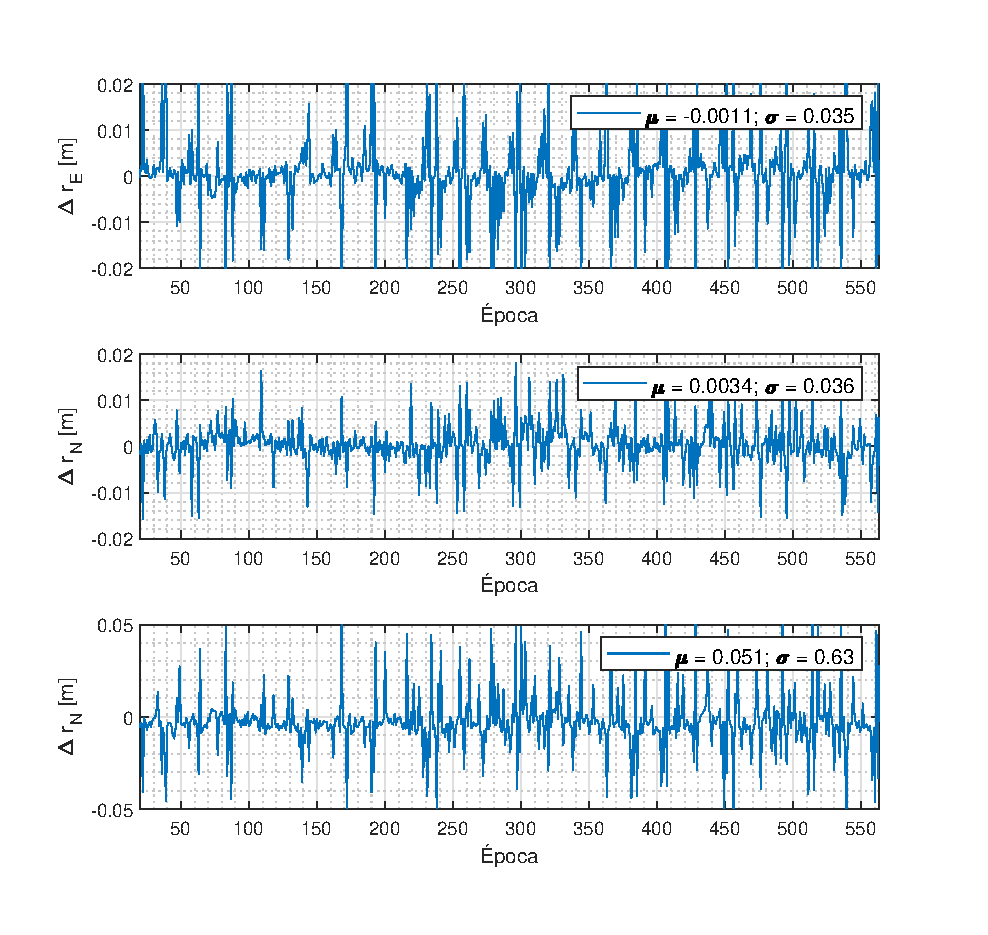
\includegraphics[width=0.7\textwidth]{/validacion/FIX_time_ENU.eps}
 	\caption{Error ENU de línea base.}
  	\label{fig:error_fix_DGNSS_Q}
\end{subfigure}
\caption{Ensayo RTK con línea de base nula operando a doble frecuencia, sistema GPS, antena SENyT, con diez satélites en vista y receptor base Serie Q.}
\label{fig:ensayoDGNSS_fix_Q}
\end{figure}
	
	Ya se mencionó que el receptor utilizado solo puede operar con las señales L1C y L2L (nombradas según RINEX). Como la comparación natural en esta sección corresponde con los ensayos RTK realizados entre dos receptores comerciales \textit{u-blox} (ver Sección~\ref{sec:RTK_ublox}), cabe destacar que ese ensayo se realizó con las señales L1C y L2C. Esto no genera inconvenientes pero es un cambio en las condiciones de ensayo impuesto por las limitaciones que presenta el receptor utilizado como base.
	
	Aquí el rover intentará resolver ambigüedades flotantes mediante técnicas como las presentadas en el Capítulo~\ref{ch:DGNSS}, en caso de tener éxito con esto procederá a resolver las ambigüedades enteras y fijarlas. Es interesante observar cómo resultan los errores en cada coordenada ENU de la línea base al inicio del ensayo mientras intenta resolver las ambigüedades (ver Fig.~\ref{fig:trans_float_fix_DGNSS_Q}). La evolución de cada coordenada converge a un valor centrado en cero, a partir de la época número siete, es decir, 7 segundos luego de comenzar el ensayo, se logran fijar las ambigüedades y el error en cada coordenada disminuye notablemente. El detalle de cada coordenada una vez que se logró resolver ambigüedades se puede observar en la Fig.~\ref{fig:error_fix_DGNSS_Q}.
		
	Los resultados de este ensayo presentados de igual manera que para los ensayos anteriores se pueden observar en la Fig.~\ref{fig:ensayoDGNSS_fix_Q}. Se obtiene una mejora considerable con respecto al ensayo donde no se utilizan mediciones de fase, esto es esperable ya que al resolver las ambigüedades se consigue utilizar las mediciones de fase de portadora como mediciones de rango pero con errores al nivel de los centímetros. Es de interés analizar la nube de soluciones obtenidas ya que se puede distinguir a grandes rasgos dos nubes, una exterior y otra interior. La nube exterior puede ser circunscrita en una circunferencia de 5\,cm de radio aproximadamente y se mantiene la diferencia entre las proyecciones que ya se discutió reiteradamente a lo largo de este trabajo. En cuanto a la nube interior, sucede lo mismo pero la circunferencia tiene un radio de 1\,cm o incluso menos. 
	
	Es necesaria una distinción entre ambas nubes ya que las mediciones tiene valores anómalos, esto se puede observar tanto en el gráfico de dispersión (Fig.~\ref{fig:scatter_fix_DGNSS_Q}) como en el error de cada coordenada (Fig.~\ref{fig:error_fix_DGNSS_Q}). En los errores de cada coordenada se presentan como los picos que existen casi de manera periódica y hacen que la varianza del error crezca considerablemente. La nube interior o más densa corresponde a las soluciones de posición sin tener en cuenta estos valores anómalos. Y se condice con los valores obtenidos en el error de cada coordenada de la Fig.~\ref{fig:error_fix_DGNSS_Q} (sin tener en cuenta los picos).
	
	Como estos resultados son los mismos al repetir el ensayo, se puede atribuir este comportamiento al receptor serie Q que es utilizado como estación base. En trabajos anteriores se ha observado un comportamiento no esperado en la generación de las mediciones de fase de portadora en la frecuencia L1. En particular, se observaba que las ambigüedades de las mediciones no eran constantes, sino que presentaban una deriva. De esta manera se puede explicar que cada vez que la deriva de las ambigüedades hace que la medición de fase crezca de manera tal que incrementa el valor entero de ambigüedades en uno, se observa una solución de posición anómala o un pico en el error de las distintas coordenadas.
	 
	El desempeño obtenido no llega a los mismos valores que en el caso en que se trabajo con dos receptores \textit{u-blox} comerciales. Esto se explica debido a las diferencias que evidentemente existen en la generación de las mediciones de fase entre ambas bases, ya que estas son las que introducen la precisión más fina. Pero sigue existiendo ganancia considerable en el desempeño obtenido respecto a un esquema de posicionamiento absoluto.
\section{Ensayo RTK con línea de base no nula}
	A modo de realizar una prueba de desempeño en una configuración más desafiante, se decide realizar un ensayo donde la línea de base ya no sea nula. Como ya se mencionó en este trabajo, el receptor Serie Q solo cuenta con una interfaz cableada UART para la comunicación RTCM. Por esto mismo, se hizo especial foco a esquemas diferenciales con línea base nula. Pero para poder dar otro tipo de validación al desarrollo llevado a cabo aquí, se hace uso de una interfaz UART a WiFi desarrollada en el lugar de trabajo para la transmisión de los mensajes RTCM a mayores distancias que las planteadas hasta ahora.

	La interfaz utilizada es implementada en dos sistemas embebidos con un módulo WiFi integrado. Uno de los dos actúa como servidor y el otro como cliente, de esta manera se envían de manera inalambrica los paquetes de datos que ingresan como UART cableada desde el receptor Serie Q qye actúa como base. Y una vez recibidos se vuelven a convertir a una interfaz UART cableada para ingresar al rover \textit{u-blox}. De esta manera es posible alejar el rover de la estación base, donde esta última no puede ser desplazada ya que trabaja con una antena bien caracterizada en cuanto a su posición.
	
	Al agregar una línea de base distinta de cero es necesario trabajar con una antena más. Para eso se utiliza una antena GNSS activa, multibanda, provista por el fabricante \textit{u-blox} junto con la placa de evaluación utilizada y tratada en el Capítulo~\ref{ch:ublox}. La antena del rover se coloca aproximadamente a una distancia estimada de 14.5\,m en el plano horizontal de la antena SENyT, esto se logra estimar en un piso inferior del Departamento de Electrotecnia donde se puede realizar la medición de distancia conociendo las proyecciones de los puntos en donde se ubica cada antena. La diferencia de alturas que presenta es aproximadamente de 3.5\,m ya que la misma es cercana a un piso estándar de un edificio. De esta manera se obtiene una longitud de la línea de base de 14.9\,m, el calculo se puede realizar ya que conocemos los catetos del triangulo rectángulo formado entre las dos antenas. 
\begin{figure}[t]
\centering
 	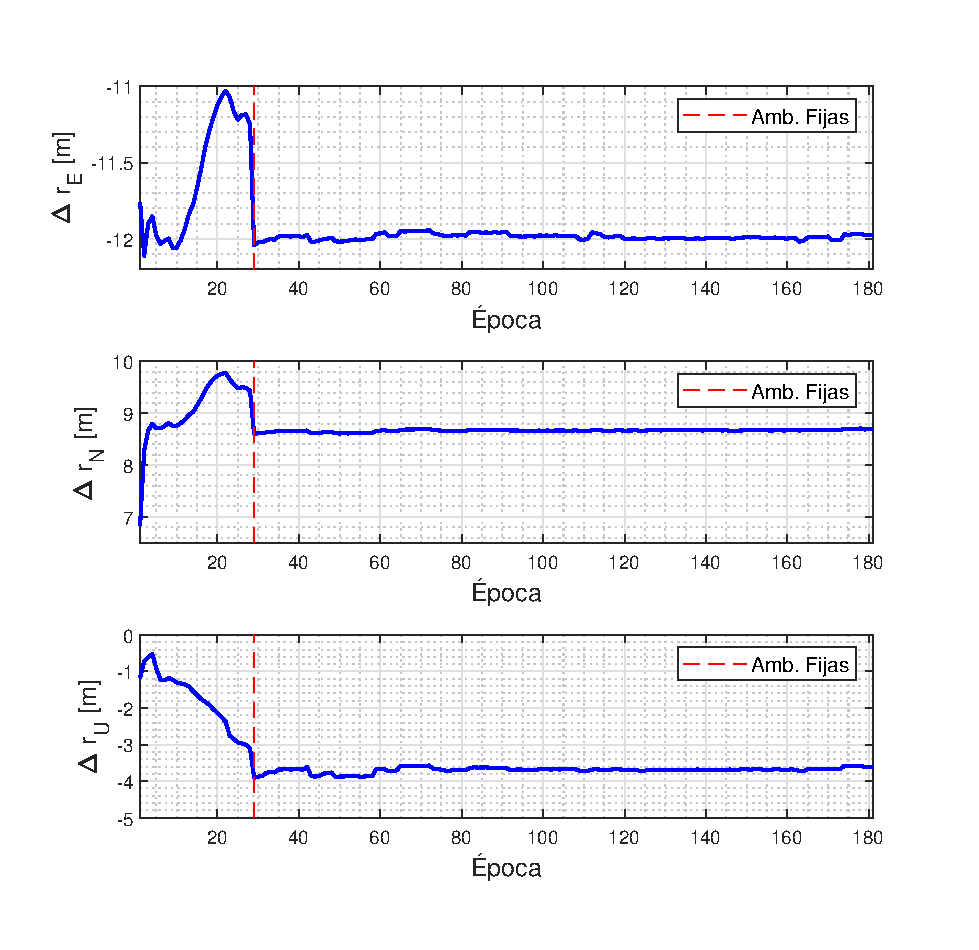
\includegraphics[width=0.7\textwidth]{/validacion/NZB/time_toFIX_NZB.eps}
 	\caption{Solución de posición relativa en coordenadas ENU mientras intenta resolver ambigüedades. Ensayo RTK con línea de base no nula y receptor base Serie Q.}
  	\label{fig:time_toFIX_NZB}
\end{figure}
	Los cálculos antes mencionados se realizan de manera aproximada ya que al trabajar en el techo de un edifico no es posible realizar la medición exacta con los equipos de los que se tiene disponibilidad. Ademas, por la ubicación de la antena SENyT y por cuestiones de alcance de la red WiFi que realiza la comunicación RTCM, no es posible elegir una ubicación de mayor comodidad para situar la antena del rover.
	
	Una vez explicadas las condiciones de realización del ensayo, se pueden presentar los resultados para comparar con los ensayos ya realizados en condiciones ideales de línea de base nula. Se toman datos por aproximadamente 10 minutos, con mediciones cada 1 segundo, para ser específicos se cuenta con 604 épocas. Los receptores operan a doble frecuencia, con la antena SENyT en la base y la antena \textit{u-blox} en el rover. En este ensayo tiene particular interés analizar el tiempo que le lleva al receptor conseguir entrar en un modo de resolución de ambigüedades, esto mismo puede ser observado en la Fig.~\ref{fig:time_toFIX_NZB}. Se comienza a guardar datos desde que se establece el enlace RTCM, es decir, el rover entra en modo 3D/DGNSS. El receptor comienza a intentar resolver ambigüedades a partir de ese momento, las condiciones no son las óptimas ya que no existe una cancelación total de todos los términos debido a la línea de base no nula. Esto explica por qué se observan desviaciones en las primeras épocas respecto a la posición de estabilización una vez que se resolvieron las ambigüedades. La variación en las coordenadas horizontales es de aproximadamente 1 metro, en cambio en la coordenada vertical se llega a tener una desviación de hasta 3 metros. Se siguen observando los inconvenientes que trae la resolución de la posición en la coordenada vertical. 
	
	A partir de la época número 29 (indicada en línea punteada en la Fig.~\ref{fig:time_toFIX_NZB}) el rover logra resolver ambigüedades enteras y fijarlas, entrando en modo 3D/DGNSS/FIXED. Aquí es donde se observa la estabilización de las coordenadas ENU de la solución de posición en el valor que corresponde para la línea de base dada. Una vez que el receptor está operando en este modo de manera estable se puede realizar un gráfico de dispersión de las soluciones ENU de la posición relativa (ver Fig.~\ref{fig:scatter_NZB}).

\begin{figure}
\begin{subfigure}{1\linewidth}
\centering
  	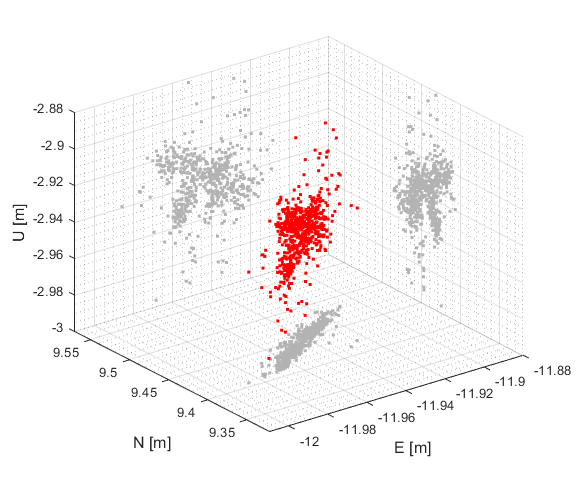
\includegraphics[width=0.7\textwidth]{/validacion/NZB/scatter_NZB.png}
  	\caption{Gráfico de dispersión ENU de las soluciones de posición relativa (línea base).}
    \label{fig:scatter_NZB}
\end{subfigure}

\begin{subfigure}{1\linewidth}
\centering
 	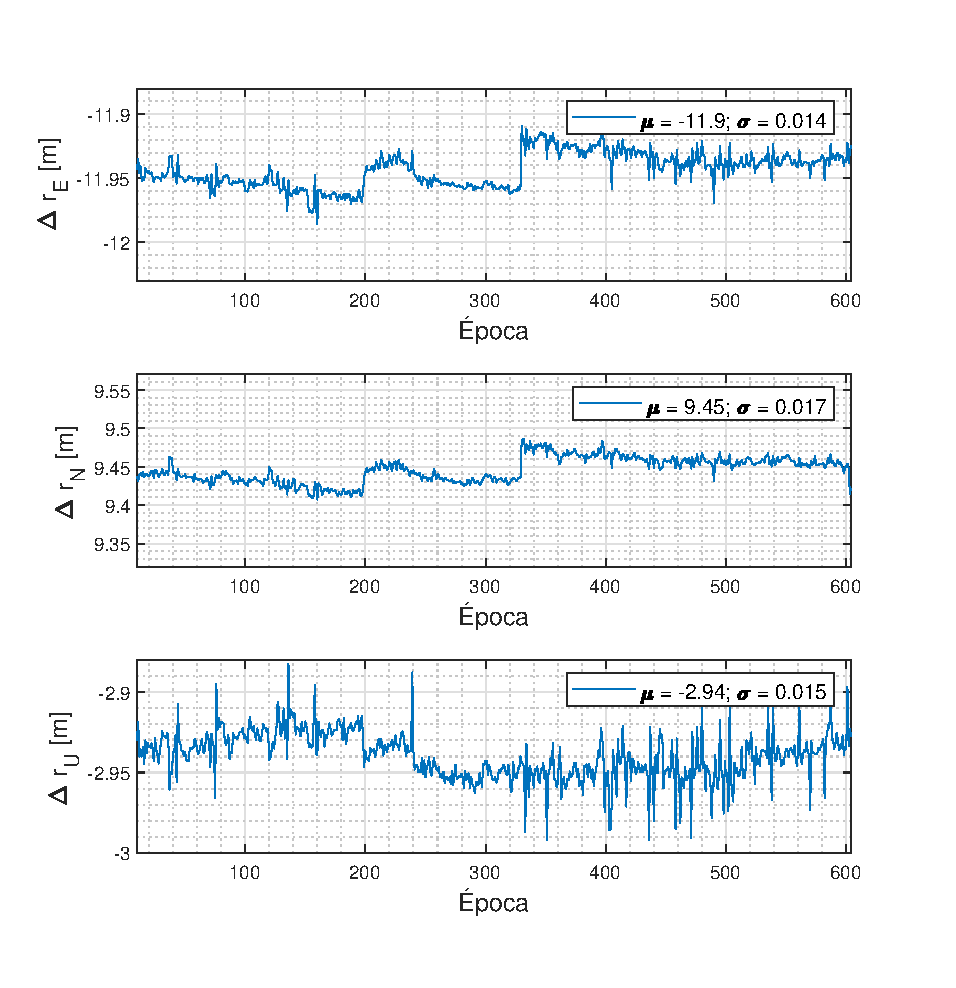
\includegraphics[width=0.7\textwidth]{/validacion/NZB/time_fix_NZB.eps}
 	\caption{Solución de posición relativa en coordenadas ENU.}
  	\label{fig:time_fix_NZB}
\end{subfigure}
\caption{Ensayo RTK con línea de base no nula operando a doble frecuencia, sistema GPS, antena SENyT en base y antena \textit{u-blox} en rover, con nueve satélites en vista y receptor base Serie Q.}
\label{fig:ensayo_NZB}
\end{figure}

	Las soluciones de posición obtenidas pueden ser circunscritas en una circunferencia de radio entre 5\,cm para todas las coordenadas. Es un resultado similar al que se obtuvo para el ensayo de línea base nula de la Sección~\ref{sec:RTK_fix_Q} al considerar la nube exterior de soluciones. Aquí no se observan soluciones como las consideradas anómalas en la sección ya mencionada, y lo mismo será corroborado al discutir el comportamiento temporal de cada coordenada de la solución (ver Fig.~\ref{fig:time_fix_NZB}). Es esperable que la precisión empeore por el hecho de no tener una línea de base nula, esto se debe a la misma razón por la que el tiempo para entrar en modo RTK es mayor en este ensayo.

	Al graficar la evolución temporal (época a época) de cada coordenada de la posición relativa (Fig.~\ref{fig:time_fix_NZB}) se observa que no existen los picos que se observaban en la Fig.~\ref{fig:error_fix_DGNSS_Q} de la sección anterior. Los ensayos en los que se reproducían los resultados con los picos o valores anómalos ya mencionados, siempre fueron con esquemas de línea base nula. Aquí en gran medida se logra reducir este efecto en algunas coordenadas. En particular, tienen mayor peso en la coordenada vertical, pero incluso se consigue ver cómo la desviación estándar en las tres coordenadas es cercana a 1.5\,cm. La contribución de las mediciones anómalas es mucho menos significativa en este esquema de línea de base no nula, que obtenía desviaciones mayores en las tres coordenadas.
	
	También se puede analizar qué tan cercana esta la línea de base estimada al ubicar las antenas con la que obtiene el receptor. Teniendo en cuenta el valor medio de cada coordenada de la Fig.~\ref{fig:time_fix_NZB} se obtiene que la línea de base tiene una distancia de 15.47\,m. El valor obtenido es muy similar a lo que se estimó anteriormente (14.9\,m) y teniendo en cuenta el método rudimentario con la que se obtuvo este último valor, es completamente aceptable la diferencia entre ambos.
\section{Conclusiones}
	Se consiguió validar el enlace de comunicación RTCM implementado en el receptor serie Q mediante ensayos con un rover comercial. Los resultados presentados para el tiempo de cómputo requerido por las rutinas que se agregan al receptor, son aceptables incluso en escenarios de procesamiento desafiante para el sistema embebido. Además, se mostró una comparación del desempeño en términos de precisión de la solución de posición para un enfoque diferencial basado en pseudorango y otro basado en mediciones de fase. Los resultados obtenidos para el posicionamiento relativo muestran las ventajas del mismo incluso al no aprovechar toda su potencialidad y conseguir resolver las ambigüedades enteras en las mediciones de fase. Se obtiene una precisión dos órdenes de magnitud menor que en los enfoques absolutos. El protocolo se encuentra completamente implementado y funcional.
	
	Si bien un escenario de receptores operando en modo DGNSS con una línea de base nula no tiene real utilidad práctica, la validación de la implementación se puede realizar de este modo. Pero para completar de validar el desarrollo y poder dar cuenta del desempeño que obtiene el mismo en un esquema con valor práctico, se ensaya con los receptores separados aproximadamente 15\,m. Se obtuvieron mejoras en los resultados comparado al caso de línea base nula debido a que la contribución que degradaba la señal en los ensayos anteriores deja de tener tanto peso en este escenario. Esto se obtiene a costa de esperar un mayor tiempo para conseguir que el receptor llegue a una operación RTK con resolución de ambigüedades, debido a las condiciones más desafiantes que presenta el escenario aquí planteado.
	
	Por último, se dejó en evidencia que una vez implementado el protocolo de comunicación RTCM en el receptor Serie Q, la decisión de diseño para la capa física es un problema aislado. El modo de operación es equivalente para una interfaz cableada como para la inalámbrica.
	
\renewcommand{\chaptermark}[1]{\markboth{\MakeUppercase{#1}}{}}	% Se le saca el num de cap al header.
\cleardoublepage
\chapter*{Conclusiones generales}\label{ch:conclusion}\chaptermark{Conclusiones generales}
\addcontentsline{toc}{chapter}{Conclusiones generales}

	El presente trabajo se desarrolla bajo la premisa de obtener un receptor Serie Q que pueda operar como estación de referencia estacionaria en un esquema DGNSS. Dando lugar a realizar ensayos y obtener resultados en tiempo real, cosa que antes solo se lograba hacer mediante post procesamiento. Esto es debido a que no existía un enlace para que el receptor realice esta comunicación. 
	
	Se estudiaron los fundamentos y hasta incluso detalles finos del posicionamiento basado en sistemas GNSS, temática que era desconocida hasta el momento de comenzar con el trabajo. A esto se le suma la familiarización y profundización con las técnicas de posicionamiento relativo, poniendo foco en los mecanismos empleados para conseguir los resultados que son conocidos tanto en la literatura como en la práctica. Efectivamente es posible obtener precisiones en el órden de los centímetros, pero a costa de tener que operar con dos (o más) receptores en simultaneo. El estudio de técnicas de posicionamiento diferencial se realiza paralelamente con el estudio del estándar RTCM para comprender las sutilezas existentes en enfoques diferenciales.
	
	Se obtienen los aspectos más importantes a tener en cuenta a la hora de pensar en un enlace de comunicación entre receptores para que operen en modo diferencial. Se le da particular importancia al enlace entre receptores de distinto modelo y fabricante, para cumplir con uno de los objetivos particulares de este trabajo. Se corrobora lo estudiado respecto a posicionamiento relativo y los aspectos relevantes extraídos del estándar replicando ensayos diferenciales con receptores comerciales, los resultados son como se esperaba. 
	
	Posterior a la etapa de estudio y replicado de ensayos se procede a la familiarización con un receptor de desarrollo propietario en el lugar de trabajo para la posterior implementación del enlace de comunicación RTCM en el mismo. El receptor aquí mencionado es utilizado como estación de referencia estacionaria y un receptor comercial como receptor móvil, se obtienen mejoras en términos de precisión en la solución de posición obtenida. 
	
	No se consigue replicar los mismos resultados conocidos en la literatura y obtenidos para un par de receptores comerciales operando en conjunto, para el caso de un escenario con línea de base nula. Se explica este desempeño obtenido debido a características del receptor propietario utilizado. En un caso de utilidad práctica como lo es cuando los receptores utilizan antenas distintas y separadas físicamente, se logra mejorar el desempeño. Concluyendo que el efecto de la generación de mediciones del receptor propietario utilizado deja de tener tener el mismo peso que en el ensayo con línea de base nula.
	
	Cabe destacar que al trabajar con un receptor de diseño y desarrollo propio del lugar de trabajo, el mismo se encuentra en constante desarrollo y mejora. Es por esto que es esperable encontrar que no tiene el mismo desempeño que un receptor comercial con altas prestaciones como el que se utilizó en este trabajo. De igual manera, en este enfoque diferencial se obtienen resultados con una precisión dos órdenes de magnitud menor que al realizar posicionamiento absoluto. Por todo esto es que se puede concluir que se consigue cumplir el objetivo general de este trabajo, tanto como los particulares. 
	
\section*{Trabajo a futuro}
\addcontentsline{toc}{section}{Trabajo a futuro}
	La línea de trabajo a futuro inmediata a partir de aquí, es la modificación de la capa física del enlace establecido. De manera que se puedan realizar ensayos a distancias de línea de base mucho mayores que dejen en evidencia cómo deja de presentar ganancias un esquema de posicionamiento relativo. Además, la implementación de nuevos mensajes para poder realizar distintos tipos de posicionamiento relativo, tiene un gran atractivo. Se podría pensar en enfoques más precisos o donde existen compromisos en cuanto a la velocidad de transmisión de los mensajes RTCM.
	
	Por otro lado, se precisa implementar los algoritmos de procesamiento diferencial en un receptor del mismo tipo. De esta manera se podrían plantear nuevos ensayos con dos receptores Serie Q realizando posicionamiento relativo en tiempo real. 
	
	Siendo aún más ambiciosos, se puede extender el enfoque RTK aquí logrado a uno del tipo red RTK. Debiendo contar con varias estaciones de referencia estacionarias para que el rover pueda recibir mensajes de múltiples bases. También se puede pensar en trabajar con estaciones base móviles, y que el posicionamiento relativo sea entre receptores que se encuentran todos en movimiento. Esto podría ser el caso de satélites de órbita baja volando formación, donde pensar en una base estacionaria es más complejo.

%\chapter*{Anexo I}\label{ch:anexo}
%% Please add the following required packages to your document preamble:
%% \usepackage[table,xcdraw]{xcolor}
%% If you use beamer only pass "xcolor=table" option, i.e. \documentclass[xcolor=table]{beamer}
%\begin{table}[]
%\begin{tabular}{|l|c|c|c|}
%\hline
%\rowcolor[HTML]{9B9B9B} 
%\multicolumn{1}{|c|}{\cellcolor[HTML]{9B9B9B}ID}              & Resolución                       & Rango                                             & Tipo de dato \\ \hline
%DF002                                                         & 1                                & 0-4095                                            & uint12       \\ \hline
%DF003                                                         & 1                                & 0-4095                                            & uint12       \\ \hline
%DF004                                                         & 1\,ms                            & 0-604799999\,ms                                   & uint30       \\ \hline
%\begin{tabular}[c]{@{}l@{}}DF025\\ DF026\\ DF027\end{tabular} & 0.0001\,m                        & $\pm$13743895,3471\,m                             & int38        \\ \hline
%DF364                                                         & 1                                & 0-3                                               & bit(2)       \\ \hline
%DF397                                                         & 1\,ms                            & 0-254\,ms                                         & uint8        \\ \hline
%DF398                                                         & $2^{-10}$\,ms                    & 0 a (1-$2^{-10}$)\,ms                             & uint10       \\ \hline
%DF399                                                         & 1\,m/s                           & $\pm$8191\,m/s                                    & int14        \\ \hline
%DF400                                                         & $2^{-24}$\,ms (aprox. 0.018\,m)  & $\pm(2^{-10}-2^{-24})$\,ms (aprox. $\pm$0.018\,m) & int15        \\ \hline
%DF401                                                         & $2^{-29}$\,ms (aprox. 0.0006\,m) & $\pm(2^{-8}-2^{-29})$\,ms (aprox. $\pm$1171\,m)   & int22        \\ \hline
%DF402                                                         & 1                                & 0-15                                              & uint4        \\ \hline
%DF403                                                         & 1\,dB/Hz                         & 1-63\,dB/Hz                                       & uint6        \\ \hline
%DF420                                                         & 1                                & 0-1                                               & bit(1)       \\ \hline
%\end{tabular}
%\end{table}
\begin{thebibliography}{00}
\bibitem{kaplan} Elliot D. Kaplan, Christopher J. Hegarty, ``Understandign GPS: Principles and Applications'', 2nd ed., Artech House.
\bibitem{proakis} John G. Proakis, Masoud Salehi, ``Digital Communications'', 5th ed., McGraw Hill.
\bibitem{rinex} IGS, Estándar RINEX 3.05, Dec. 2020.
\bibitem{handbook} Peter J.G. Teunissen \& Oliver Montenbruck (eds.), ``Handbook of Global Navigation Satellite Systems'', Springer.
\bibitem{utc} The United States Naval Observatory, Data Products, UTC, \href{https://crf.usno.navy.mil/ut1-utc}{https://crf.usno.navy.mil/ut1-utc}.
\bibitem{psiakis} Mark L. Psiaki and S. Mohiuddin, ``Modeling, Analysis, and Simulation of GPS Carrier Phase for Spacecraft Relative Navigation'', \textit{Journal of Guidance, Control, and Dynamics}, vol. 30, num. 6, 2007, pp. 1628-1639.
\bibitem{bart} Garcia, Javier G. and Roncagliolo, Pedro A. and Muravchik, Carlos H., ``A Bayesian Technique for Real and Integer Parameters Estimation in Linear Models and Its Application to GNSS High Precision Positioning'', IEEE Transactions on Signal Processing, vol. 64, no. 4, 2016, pp. 923-933.
\bibitem{rtcm} Comisión Radio Técnica para Servicios Marítimos, Estándar RTCM 10403.3, Versión 3.
\bibitem{ZEDds} u-blox, ``u-blox F9 high precision GNSS module'', ZED-F9P data sheet, Jun. 2020, [rev. R08].
\bibitem{C099_ds} u-blox, ``Application board ZED-F9P ODIN-W2'', C099-F9P user guide, Jun. 2020, [rev. R12].
\bibitem{u_center} u-blox, ``GNSS evaluation software for Windows'', u-center user guide, Oct. 2021, [rev. R28].
\bibitem{moving_base_AppN} u-blox, ``Moving base applications'', App. Note, Jul. 2020, [rev. R02].
\bibitem{Qseries_1} Rodríguez Santiago, Ramón López La Valle, Gerardo Puga, Javier G. García y Pedro A. Roncagliolo, ``Design of a dual-antenna and dual-band GPS receiver for CubeSats'', Congreso de IEEE Uruguay, URUCON 2017, Montevideo, Uruguay. ISBN: 978-1-5386-3397-7.
\bibitem{Qseries_2} Rodríguez Santiago, García Javier G., Scillone Germán, Díaz Juan G., López La Valle Ramón, Martire Lucas y Roncagliolo Pedro A., ``Receptor GNSS satelital con factor de forma CubeSat'', X Congreso de Tecnología Espacial CATE 2019, Anales del congreso, Buenos Aires, Argentina.
\bibitem{correlation} Pedro A. Roncagliolo, Javier G. García, Carlos H. Muravchik, ``Carrier Phase Discrimination for a Common Correlation Interval GNSS Receiver Architecture'', International Journal on Advances in Telecommunications, vol. 5, no. 3 \& 4, 2012, pp. 264-273.
\bibitem{rtklib} T. Takasu, ``RTKLIB: An Open Source Program Package for GNSS Positioning'', RTKLIB v. 2.4.2 manual, 2013.
\end{thebibliography}

\end{document}
%Revisar todo esto!!!
%=============================================================================
%